  \documentclass[11pt]{article}
\usepackage{debulletin}
%\usepackage{deauthor}
\usepackage{times}
\usepackage{epsfig}
%\usepackage{subfigure}
\usepackage{wrapfig}
\usepackage{color}
\usepackage{boxedminipage}
\usepackage{graphicx}
\usepackage{url}
\usepackage{tabu}
\usepackage{multirow}
\usepackage{ulem}
\usepackage{layouts}
\usepackage[utf8]{inputenc}
\usepackage{paralist}
%\usepackage{thmtools} 
\usepackage{thm-restate}
\usepackage{dsfont}
%\usepackage{amsthm}
\usepackage{amsmath}
\usepackage{amssymb}
\usepackage{amsfonts}
\usepackage{hyperref}
\usepackage{enumitem}
\usepackage{xspace}
\usepackage{tikz}
\usepackage[T1]{fontenc}
\usepackage{beramono}
\usepackage{listings}
\usepackage{xcolor}
\usepackage{graphics}
\usepackage{pifont}
\usepackage{algorithmic}
\usepackage[sort&compress,numbers]{natbib}
\usepackage{microtype}
\usepackage{booktabs}
\usepackage{pgfplotstable}
\usepgfplotslibrary{groupplots}
\usepackage{bbm}
\usepackage{verbatim}
\usepackage{caption}
\usepackage{subcaption}
\usepackage{siunitx}
\usepackage[autostyle, english=american]{csquotes}
\usepackage{breakurl}
\usepackage{makecell}
\usepackage{changepage}
\usepackage{diagbox}
\usepackage{etoolbox}
\usepackage{float}
\usepackage{array}
\usepackage{tabularx}
\usepackage{colortbl}
\usepackage[english]{babel}
\usepackage[edges]{forest}
\usepackage{xfrac}
\usepackage{mdwlist}
\usepackage{arydshln}
\usepackage{adjustbox}
\usepackage{longtable}
\usepackage{comment}
\usepackage{svg}
\usepackage[vlined,ruled,linesnumbered]{algorithm2e}
\usepackage{bm}
\usepackage[noend]{algpseudocode}
\usepackage{soul}
\usepackage{makecell}
\usepackage{cleveref}
\usepackage{grffile}
\usepackage{tablefootnote}
\usepackage{threeparttable}
\usepackage{bibentry}
\usepackage{cancel}
\usepackage[sectionbib]{chapterbib}

\DeclareMathOperator*{\argmin}{argmin} 
\DeclareMathOperator*{\argmax}{argmax} 
% \newcommand{\xhdr}[1]{{\vspace{1pt}\noindent\bfseries #1}.}
% \newcommand{\ie}{\textit{i.e., }}
% \newcommand{\eg}{\textit{e.g., }}
% \newcommand{\etal}{\textit{et al.}}
% \newcommand{\etc}{\textit{etc.}}
% \newcommand{\wrt}{\textit{w.r.t. }}
% \newcommand{\cf}{\textit{cf. }}
% \newcommand{\aka}{\textit{aka. }}
% \newcommand{\CITE}{\textcolor{blue}{(CITE)}}
% \newcommand{\rex}[1]{\textcolor{magenta}{(Rex: #1)}}
% \newcommand{\jialin}[1]{\textcolor{olive}{(Jialin: #1)}}

\definecolor{citecol}{HTML}{2DDC0E}
\definecolor{tableofcontent}{HTML}{E63E15}
\definecolor{urlcol}{HTML}{2470D8}
\usepackage{hyperref}
\hypersetup{
    colorlinks=true,       % false: boxed links; true: colored links
    linkcolor=tableofcontent, 
    citecolor=citecol,        % color of links to bibliography
    %filecolor=blue,      % color of file links
    urlcolor=black,           % color of external links
}


\newcolumntype{L}[1]{>{\raggedright\let\newline\\\arraybackslash\hspace{0pt}}m{#1}}
\newcolumntype{C}[1]{>{\centering\let\newline\\\arraybackslash\hspace{0pt}}m{#1}}
\newcolumntype{R}[1]{>{\raggedleft\let\newline\\\arraybackslash\hspace{0pt}}m{#1}}

\newenvironment{CompactEnumerate}{
\begin{list}{\arabic{enumi}.}{%
\usecounter{enumi}
\setlength{\leftmargin}{14pt}
\setlength{\itemindent}{1pt}
%\setlength{\topsep}{-1pt}
\setlength{\itemsep}{1pt}
}}
{\end{list}}

\newenvironment{CompactItemize}{
\begin{list}{$\bullet$}{%
\setlength{\leftmargin}{14pt}
\setlength{\itemindent}{0pt}
%\setlength{\topsep}{-1pt}
\setlength{\itemsep}{0pt}
}}
{\end{list}}

\begin{document}


% please enter real date, vol no, issue no
\bulletindate{March 2024}
\bulletinvolume{48}
\bulletinnumber{1}
\bulletinyear{2024}

% these are files that I have- but your part of the issue can be done without
% them
\IEEElogo{cs.pdf}
\insidefrontcover{incvA19.pdf}
%\insidebackcover[ICDE Conference]{./calls/icde-new-a.ps}

\begin{bulletin}

% the above samples assume the issue is generated from a directory structure of the following sort
% major directory name is month and year of issue
% there are sub-directorys for
% letters: directory name is "letters"
% technical articles: a directory per paper, named for an "author"
% news articles: directory name is "news"
% calls: directory name is "calls

%
%  Editor letters section.  Use the lettersection environment.
%  Each letter is contained in a letter environment, where the two required
%  options to \begin{letter} are the author and the address of the author.
%

\begin{lettersection}

% there will be other letters- and a blank page will appear in your document
% but the special issue part will be fine

\begin{letter}{Letter from the Editor-in-Chief}
 {Haixun Wang}{Instacart}
 \documentclass[11pt]{article} 

\usepackage{deauthor,times,graphicx}
%\usepackage{url}
\usepackage{hyperref}

\begin{document}
How to efficiently and effectively manage large-scale data is a
critical challenge in data management, scientific computing, machine
learning, and many other fields. In this issue, we look into this
problem from two angles.

Gerhard Weikum's opinion piece titled ``Entities with Quantities''
highlights development along the direction of querying the Web as a
database. We have come a long way in keyword based Web search: Today,
all major search engines support entity based question/answering to
certain extent (e.g., returning ``Eiffel Tower'' for query ``the
highest building in Paris''). Weikum is taking one important step
towards the goal of querying the Web as a database. In the article, he
discusses what it takes to find all entities that satisfy a
quantity-based search condition, for example, ``buildings taller than
500m'' or ``runners completing a marathon under 2:10h.''  It is clear
that this requires much advanced data preprocessing (e.g., information
extraction, entity linking, etc.), but more importantly, it requires
that at least part of the data on the entire Web needs to be organized
as a database.

Philippe Bonnet put together the current issue consisting of 5 papers
from leading researchers in the high performance computing and data
management communities on the topic of data management at
Exascale. Advances in exascale computing on petascale supercomputers
are pushing the frontier of scientific computing that requires complex
simulation, benefiting applications ranging from astrophysical
discovery to drug design. But with increasing amounts of data, the gap
between computation and I/O has grown significantly wider, which makes
data management a big challenge. This timely issue answers many
questions in this domain.

\end{document}


\end{letter}

\newpage


\newpage


% your introductory letter goes here

\begin{letter}{Letter from the Special Issue Editor}
%\begin{letter}{Letter from the Special Issue Editors} %JF: made it editors, plural
%\setcounter{section}{0}
{Steven Euijong Whang}{Korea Advanced Institute of Science and Technology}
\documentclass[11pt]{article}

\usepackage{deauthor,times,graphicx}
%\usepackage{url}

\begin{document}
Graph Neural Networks (GNNs) have propelled the field of graph-based machine learning, unlocking new and innovative applications in various domains, such as natural language processing, drug discovery, recommendation systems, and social network analysis. By leveraging the graph structure and node features, GNNs capture intricate relationships and dependencies in complex networks, resulting in more accurate predictions and a deeper understanding of the data. These advancements have led to significant breakthroughs in drug design, personalized recommendations, and community detection in social networks. Moreover, GNNs’ ability to model and analyze structured data has opened up new avenues for advancing artificial intelligence. Particularly, integrating GNNs with large language models (LLMs) will elevate their capabilities by incorporating world knowledge from LLMs and enabling natural language querying of graph-structured data. These advancements are poised to reshape the landscape of GNN research, paving the way for exciting possibilities and future advancements.

Despite their promise, GNNs have limitations. These include challenges in generalizing to unseen graph structures, scalability issues with large-scale graphs, difficulties in handling heterophily, limited interpretability resulting in black-box behavior, complexities in data requirements and feature engineering, as well as concerns regarding over-smoothing and potential loss of discriminative information. In this special edition, seven carefully selected papers address these limitations and offer insights into improving GNNs.

Graph based machine learning has been centered on the premise of similar nodes have a stronger relationship. Heterophily breaks this assumption. The first article by {\bf Zhu et al.}, titled “Heterophily and Graph Neural Networks: Past, Present, and Future,” investigates the performance of GNNs on graphs exhibiting heterophily. The authors review various GNN designs proposed for handling heterophilous graphs and explore their connections to research objectives like robustness, fairness, and over-smoothing avoidance. They emphasize the need for tailored GNN designs specific to heterophily.

Explainable GNN models are often necessary for legal, regulatory, and compliance purposes. Two articles in this edition focus on the explainability of GNN models. {\bf Kakkad et al.}’s “A Survey on Explainability of Graph Neural Networks” offers a comprehensive overview of explainability techniques for GNNs, categorizing them based on objectives, methodologies, and application scenarios. {\bf Rex Ying}’s paper, “Generative Explanation for Graph Neural Networks: Methods and Evaluation,” proposes a unified optimization framework for generative explanation methods, highlighting the shared characteristics and distinctions among these approaches.

Representation learning is an important topic in GNN research, and this edition features two articles that delve into this topic. First, {\bf Han et al.} presents a graph contrastive learning (GCL) framework aimed at learning graph representations of homogeneous, heterogeneous, and hypergraphs. They discuss improvements in principled view generation, which contribute to generalizability, fairness, and interpretability. Next, {\bf Seshadri}'s paper highlights the limitations of low-dimensional embeddings in learning representations. The work presents theoretical underpinnings showing how low-dimensional embeddings cannot capture the fine-grained community structure of real-world data.

Finally, {\bf Wang et al.} presents the concept of “Customized Graph Neural Networks.” They propose a novel framework, Customized-GNN, which generates sample-specific GNN models for individual graphs based on their structures. The authors show the effectiveness of this framework through comprehensive experiments on various graph classification benchmarks.

We believe these seven articles offer a sample of the ongoing work, recent advances, and existing limitations in the field of GNN research. By exploring various aspects of GNNs, such as performance on heterophilous graphs, explainability techniques, generative explanations, graph contrastive learning, limitations of low-dimensional embeddings, and customized GNN frameworks, these articles contribute to a deeper understanding of GNNs and their potential applications.  Our special thanks to {\bf Yoachen Xie} for their feedback on selected submissions and to {\bf Nurendra Choudhary} for their role as the web publication chair for this edition. 

%As the field of GNN research continues to evolve rapidly, these articles will serve as a valuable resource, guiding further exploration and driving advancements in this exciting domain.

\end{document}

\end{letter}

\end{lettersection}

\begin{articlesection}{Personal Information Management}
%
%  Contributed articles section.  Use the articlesection environment.
%  Each article is contained in an article environment, where the two required
%  options to \begin{article} are the title and author of the article
%
\begin{article}
{Coverage-based Data-centric Approaches for Responsible and Trustworthy AI}
{Nima Shahbazi, Mahdi Erfanian, Abolfazl Asudeh}
\setcounter{section}{0}
% link to instruction: https://tc.computer.org/tcde/tcde-bulletin-author-instructions/
% \documentclass[11pt,dvipdfm]{article}
\documentclass[11pt]{article}
\usepackage{tabularx}
\usepackage{ragged2e}  % for '\RaggedRight' macro (allows hyphenation)
\usepackage{booktabs}  % for \toprule, \midrule, and \bottomrule macros
\usepackage{textcomp}
\usepackage{amsfonts,amsmath}
\usepackage{deauthor,times}
\usepackage{graphicx} % 
\usepackage{hyperref}
\usepackage{comment}
\graphicspath{{asudeh/}}
\usepackage{soul}
\usepackage{subcaption}
\usepackage{ulem}
\usepackage{wrapfig}
\usepackage{color}
\usepackage{xspace}
\newtheorem{problem}{Problem}

%\DeclareMathOperator*{\argmax}{arg\,max}

%remove the following commands/package b4 submission
\newcommand{\hide}[1]{}
\newcommand{\eat}[1]{}
\newcommand{\resolved}[1]{\hide{#1}}
\newcommand{\abol}[1]{\textcolor{red}{Abol: #1}}
\newcommand{\mahdi}[1]{\textcolor{red}{Mahdi: #1}}
\newcommand{\nima}[1]{\textcolor{red}{Nima: #1}}

\newcommand{\dee}{\mathcal{D}}
\newcommand{\Gee}{\mathcal{G}}
\newcommand{\gee}{\mathbf{g}}
\newcommand{\ee}{\mathbf{e}}
\newcommand{\es}{\mathcal{S}}
\newcommand{\el}{\mathcal{L}}
\newcommand{\xx}{\mathcal{x}}
\newcommand{\dist}{\xi}
\newcommand{\alg}{\mathsf{A}}
\newcommand{\qu}{\mathbf{q}}
\newcommand{\ex}{\mathbf{x}}
\newcommand{\ti}{\mathbf{t}}
\newcommand{\sdt}{\mathsf{SDT}}
\newcommand{\wdt}{\mathsf{WDT}}
\newcommand{\Qu}{\mathbf{Q}}
\newcommand{\pe}{\mathbb{P}}
\newcommand{\megam}{\mathcal{M}}
\newcommand{\eps}{\varepsilon}
\newcommand{\enet}{{$\varepsilon$-{\bf net}}\xspace}
\newcommand{\net}{{\tt net}\xspace}
\newcommand{\vcd}{VC-dimension\xspace}
\newcommand{\at}[1]{{\tt \small #1}\xspace}
\newcommand{\pr}{Pr}

\newcommand{\sharpP}{\mbox{\#P}}
\newcommand{\NP}{\mathsf{NP}}
\newcommand{\LP}{\mathsf{LP}}
\newcommand{\IP}{\mathsf{IP}}
\newcommand{\ru}{{\sc {RU}}\xspace}
\newcommand{\sru}{{\sc {strongRU}}\xspace}
\newcommand{\wru}{{\sc {weakRU}}\xspace}

\newcommand{\fmsystem}{{\sc Chameleon}\xspace}
\newcommand{\fm}{$\mathcal{F}$\xspace}

\newtheorem{experiment}{Experiment}

\begin{document}

\title{Coverage-based Data-centric Approaches for \\Responsible and Trustworthy AI\thanks{This research was supported by the National Science Foundation under grant No. 2107290.}}

\author{
\begin{tabular}[t]{c@{\extracolsep{2.4em}}c@{\extracolsep{2.4em}}c@{\extracolsep{2.3em}}c} 
Nima Shahbazi & Mahdi Erfanian & Abolfazl Asudeh \\ 
University of Illinois Chicago & University of Illinois Chicago & University of Illinois Chicago\\
 nshahb3@uic.edu & merfan2@uic.edu & asudeh@uic.edu
\end{tabular}
}

\maketitle


\begin{abstract}
The grand goal of data-driven decision systems is to help make decisions easier, more accurate, at a higher scale, and also just. However, data-driven algorithms are only as good as the data they work with. Yet, data sets, especially those with social data, often do not represent minorities. The paucity of training data is a perpetual problem for AI, and the outcome of ML models for cases not represented in their training data is often not reliable. 
Hence, without properly addressing the lack of representation issues in data, we cannot expect AI-based societal solutions to have responsible and trustworthy outcomes. 

This paper focuses on data coverage as a data-centric approach for identifying and resolving misrepresentation of minorities in data.
To achieve this goal, we propose novel algorithms that (a) {\it identify} and {\it resolve} insufficient data coverage across data with different modalities and (b) use lack of representation information to generate data-centric {\it reliability warnings}.
 \end{abstract}
 
 %%%%%%%%%%%%%%%%%%%%%%%%%%%%%%%% INTRO  %%%%%%%%%%%%%%%%%%%%%%%%%%%%%%%%
\section{Introduction}\label{sec:intro} % Abstract+Intro: up to 2.5 pages 
Data-driven decision-making has shaped every corner of human life, spanning from autonomous vehicles to healthcare and even predictive policing and criminal justice. A pivotal concern, especially in applications that affect individuals, revolves around the reliability of the decisions rendered by the system.
It is easy to see that the accuracy of a data-driven decision depends, first and foremost, on the data used to make it. Essentially, the system learns the phenomena that data represent. While we may desire that the data should represent the underlying data distribution from which the production data is drawn, this alone may be insufficient, as it merely enables the model to perform well for the average case.
As a result, a model with a high accuracy could fail for specific regions in the data with insufficient representation. These regions may matter because they frequently represent some minority population in society. They could also represent cases that may not happen very often but have a relevant impact on the correctness of a critical decision.
In short, if the data fails to sufficiently represent a specific population, the outcome of the decision system for that population may not be trustworthy.

The phenomenon known as \textit{Representation Bias} can arise from how the data was originally collected, or it could be the result of biases introduced post-collection—whether historically, cognitively, or statistically.

Representation bias is essentially inevitable without a systematic approach to data collection. 
For example, in the context of survey data collection, vital steps involve identifying all populations within the underlying distribution based on desired demographic information and ensuring comprehensive coverage with sufficient samples from each group. 
Even then, only an (uncontrolled) subset of the invitees will opt-in to respond to the survey.
Another challenge lies in the fact that data scientists often lack control over the data collection process, leading to the reliance on ``found data'' in the majority of data-driven systems. Therefore, with no guarantee on the aforementioned steps in the data collection process, the found data is most likely a biased sample.
Acknowledging the potential harms of representation bias, the notion of \textit{Data Coverage}~\cite{asudeh2019assessing,shahbazi2023representation} has been proposed to ensure the adequate representation of minority groups in data sets employed for decision-making and developing sophisticated data science tools. 

Addressing representation issues in data poses various challenges depending on the modality of the data. In this paper, we focus on identifying and resolving lack of coverage issues in data with different modalities.
We start by proposing a variety of techniques (spanning from geometric and combinatorial optimization to crowd-souring) aimed at efficiently detecting insufficient coverage on structured data sets with non-ordinal categorical and continuous attributes, as well as image data sets. Next, we propose a range of approaches grounded in data integration and generative data augmentation to address the lack of coverage by enriching the data sets with more data. However, with limited control over the data collection processes, it could be difficult and expensive to resolve all misrepresentations. 
Since adding more data is not always possible, we proceed to introduce data-centric preventive solutions that warn the user about the reliability of their predictions regarding representation bias issues. These warnings assist users in determining whether they trust the outcomes of the models or exercise caution. 

 %%%%%%%%%%%%%%%%%%%%%%%%%%%%%%%% IDENTIFICATION  %%%%%%%%%%%%%%%%%%%%%%%%%%%%%%%%
\section{Detecting Insufficient Representation of Minorities}\label{sec:identification} %up to 3.5 pages
Representation bias happens when the development (training data) population under-represents 
and subsequently fails to generalize well 
for some parts of the target population, due to historical bias, sampling bias, etc.
The notion of {\it data coverage} has been studied across different settings in \cite{shahbazi2023representation} as a metric to measure representation bias. At a high level, coverage is referred to as having enough similar entries for each object in a data set. 
For a better understanding, let us go over the definition of the generalized notion of coverage:

\begin{definition}[Data Coverage]\label{def:coverage}
Consider a data set $\dee$ with $n$ tuples, each consisting of $d$ attributes of interest $\mathbf{x}=\{x_1, x_2, \cdots,x_d\}$, such as {\tt gender}, {\tt race}, {\tt salary}, {\tt age}, etc, that are used for coverage identification.
The data set also contains target attributes $\mathbf{y} = \{ y_1,\cdots,y_{d'}\}$ that may or may not be considered for the coverage problem.
A query point $q$ is not covered by the data set $\dee$, if there are not ``enough'' data points in $\dee$ that are representative of $q$.
To generalize the notion of coverage, let us define $\gee(q)$ as the universe of tuples that would represent $q$ and let $\gee_\dee(q) = \gee(q)\cap \dee$. In other words, $\gee_\dee(q)$ are the set of tuples in $\dee$ that represent $q$.
Using this notation, we define the coverage of $q$ as the size of $\gee_\dee(q)$. That is,
$cov(q,\dee) = | \gee_\dee(q)|$.
Given a value $\tau$, $q$ is covered if $cov(q,\dee)>\tau$.
Similarly, a group $\gee$ is not covered if $\gee\cap \dee<\tau$.
The {\it uncovered region} in a data set is the collection of groups that are not covered by it.
\end{definition}

\subsection{Structured Data}
In this section, we focus on identifying representation bias in structured data.
Depending on the type of the attributes of interest, we categorize the techniques into two classes based on whether they target the problem for non-ordinal {\it categorical} (e.g. {\tt race}, {\tt gender}) or ordinal {\it continuous} (e.g. {\tt age}) attributes. The attributes of interest considered for representation bias often include sensitive attributes such as {\tt race} and {\tt gender} but are not necessarily limited to them.

\subsubsection{Categorical Attributes}

For cases where attributes of interest are non-ordinal categorical,
the cartesian product of values on a subset of attributes $\mathbf{x}'\subseteq \mathbf{x}$, form a set of (sub-)groups.
For example, $\{$ {\tt white male}, {\tt white female}, {\tt black male} $,\cdots\}$ are the subgroups defined on the attributes {\tt (race,gender)}.
We refer to the number of attributes used to specify a subgroup as the {\it level} of that subgroup.
For example, the level of the subgroup {\tt white male} is 2, while the level of the subgroup {\tt male} is 1.
We use $\ell(\gee)$, to refer to the level of a subgroup $\gee$.
Similarly, we say a subgroup $\gee'$ is a subset of $\gee$, if the groups specifying $\gee'$ are a superset of the ones for $\gee$. For example {\tt (married white male)} a subset of the more general group {\tt (white male)}. That is, the set of individuals in group {\tt (married white male)} are a subset of {\tt (white male)}.
Moreover, we say a subgroup $\gee$ is a {\it parent} of the subgroup $\gee'$, if $\gee'\subset \gee$ and $\ell(\gee)=\ell(\gee')+1$. For example, the subgroup {\tt (white male)} is a parent of the subgroup {\tt (married white male)}.
We use \textit{patterns} to refer to uncovered subgroups.
A pattern $P$ is a string of $d$ values, where $P[i]$ is either a value from the domain of $x_i$, or it is ``unspecified'', specified with $X$. 
For example, consider a data set with three binary attributes of interest $\mathbf{x}=\{x_1, x_2, x_3\}$. The pattern $P=X01$ specifies all the tuples for which $x_2=0$ and $x_3=1$ ($x_1$ can have any value).
The set of patterns that identify most general uncovered subgroups are called {\it Maximal Uncovered Patterns} (MUPs).

No polynomial time algorithm can guarantee the enumeration of the entire MUPs, however, several algorithms inspired by set enumeration and the Apriori algorithm for association rule mining are proposed to efficiently address this problem~\cite{asudeh2019assessing}.
In this regard, we introduce \textit{Pattern Graph} data structure that exploits the relationship between patterns to do less work than computing all uncovered patterns by removing the non-maximal ones. 
The parent-child relationship between the patterns is represented in a graph that can be used to find better algorithms. 
\textit{Pattern-Breaker} starts from the top of the graph where the general patterns are and moves down by breaking each pattern into more specific ones. If a pattern is uncovered, then all of its descendants are also uncovered and they can not be an MUP, even if they have a parent that is covered. Therefore, this subgraph of the pattern graph can be pruned. 
The issue with \textit{Pattern-Breaker} is that it explores the covered regions of the pattern graph and for the cases where there are a few uncovered patterns, it has to explore a large portion of the exponential-size graph. 
To tackle this, \textit{Pattern-Combiner} algorithm is proposed that performs a bottom-up traversal of the pattern graph. It uses an observation that the coverage of a node at the level of the pattern graph can be computed as the sum of the coverage values of its children. 
The problem with \textit{Pattern-Combiner} is that it traverses over the uncovered nodes first and therefore, it will not perform well for the cases in which most of the nodes in the graph are uncovered. 
In fact, for the cases where most of the MUPs are placed in the middle of the graph, both \textit{Pattern-Breaker} and \textit{Pattern-Combiner} will not be as efficient as they should traverse half of the graph. Therefore, we propose \textit{Deep-Diver}, a search algorithm based on Depth-First-Search that quickly finds the MUPs, and uses them to limit the search space by pruning the nodes both dominating and dominated by the discovered MUPs.

\begin{figure*}[!tb]
    \begin{minipage}[t]{0.31\linewidth}
        \centering
        \includegraphics[width=\textwidth]{submissions/submission1/shahbazi/covcube1.jpg}
        \caption{\small Categorical attributes: the uncovered region of a toy example, as the collection of three MUPs.}
        \label{fig:covcube1}
    \end{minipage}
    \hfill
    \begin{minipage}[t]{0.31\linewidth}
        \centering
        \includegraphics[width=\textwidth]{submissions/submission1/shahbazi/cvrg_2_1.jpg}
        \caption{\small Continuous attributes, 2D: identifying the covered region in the gray Voronoi cell.}
        \label{fig:cvrg_2_1}
    \end{minipage}
    \hfill
    \begin{minipage}[t]{0.31\linewidth}
        \centering
        \includegraphics[width=\textwidth]{submissions/submission1/shahbazi/cvrg_2_2.jpg}
        \caption{ \small Continuous attributes, 2D: Uncovered region marked in red.}
        \label{fig:cvrg_2_2}
    \end{minipage}
\vspace{-5mm}
\end{figure*}

\subsubsection{Continuous Attributes}
Data in the real world often consists of a combination of continuous and discrete values. While simple solutions like binning {\tt age} into {\tt young} and {\tt old} can transform the continuous space into discrete. However, they may lead to coarse groupings that are sensitive to the thresholds chosen. It may be inappropriate to treat a 35-yo as {\tt young} but a 36-yo as {\tt old}. 
Therefore, we extend the notion of coverage to continuous space. Particularly, given data set $\dee$ with $n$ tuples over $d$ attributes, and vicinity radius $\rho$ and coverage threshold $k$, we want to identify the uncovered region -- the universe of uncovered query points.
A query point in continuous data space is covered if there are enough (at least $k$) data points in its $\rho$-vicinity neighborhood. $\rho$-vicinity neighborhood is the circle centered at the query point with radius $\rho$.

Depending on the number of attributes in a data set, we propose two algorithms for identifying uncovered regions in data~\cite{asudeh2021coverage}. 
The first algorithm known as \textit{Uncovered-2D} studies coverage over two-dimensional data sets where $\mathbf{x}=\{x_1,x_2\}$. To find the number of circles that a query point falls into and consequently discover the uncovered region, \textit{Uncovered-2D} makes a connection to $k$-th order Voronoi diagrams.
Consider a data set $\mathcal{D}$ and its corresponding $k$-th order Voronoi diagram. For every tuple $t\in \mathcal{D}$, let $\circ_t$ be the $d$-dimensional sphere ($d$-sphere) with radius $\rho$ centered at $t$.
Consider a $k$-voronoi cell $\mathcal{V}(S)$ in the $k$-th order Voronoi diagram $V_k(\mathcal{D})$.
Any point $q$ inside the intersections of the $d$-spheres of tuples in $S$, i.e. $q\in \underset{\forall t\in S}{\cap ~\circ_t}$, is covered, while all other points in the region are uncovered.
 The algorithm starts by constructing the $k$-th order Voronoi diagram of the data set and then for each Voronoi cell $\mathcal{V}(S)$ in the diagram, it computes the intersection of the circles of the tuples in $S$ and marks the portion of $\mathcal{V}(S)$ that falls outside it as uncovered.
After identifying the uncovered region, a 2D map of $\{x_1,x_2\}$ value combinations is used to report the region to the user.
The algorithm for the 2D case can be extended to the general case by relaxing the assumption on the number of attributes to discover the exact uncovered region, however, due to the curse of dimensionality, the search size space explodes as the number of dimensions increases and as a result, the algorithm will not be practical. Therefore, we propose a randomized approximation algorithm based on the geometric notion of \enet. 
Let $\mathcal{X}$ be a set and $\mathcal{R}$ be a set of subsets of $\mathcal{X}$. A set $\mathcal{N}\subset \mathcal{X}$ is an \enet for $\mathcal{X}$ if for any range $r\in\mathcal{R}$, if  $|r\cap \chi|>\eps|\chi|$, then $r$ contains at least one point of $N$.
The idea, at a high level, is to draw enough random samples from the space of potential query points to form an \enet. 
We then label the sampled query points as $\{-1,+1\}$ depending on whether those are covered or not, and learn the uncovered regions using the samples.

\subsection{Image Data}
Many known incidents of machine failures due to the lack of representation were on image data.
We consider an image data set with a fixed number of low-cardinality sensitive attributes such as {\tt\small race} and {\tt\small gender}. 
It is common that image data sets {\it lack explicit values} for sensitive attributes, which are crucial for coverage identification. An image data set is often a collection of images from different domains with little to no information about their domain and which groups they belong to. As a result, even studying coverage over low-cardinality and categorical attributes of interests is challenging in these cases.

\begin{wrapfigure}{R}{0.42\textwidth}
\centering
\vspace{-3mm}
\scriptsize
\begin{tabular}{|@{}c|@{}c@{}|@{}c@{}|@{}c@{}|} 
 \hline
{\bf data set} & {\bf classifier} & {\bf accuracy} & {\bf precision} \\ 
 &  &  & {\bf on female} \\ \hline
UTKFace:~& DeepFace (opencv) & 93.56 & {52.02}\\\cline{2-4}
({\tt females}=200,& DeepFace (retinaface) & 94.16 & {56.15}\\\cline{2-4}
{\tt males}=2800) & BaseCNN & 97.6 & 74.8\\
\hline
UTKFace:~& DeepFace (opencv) & 96.53 & {\bf 8.0}\\\cline{2-4}
({\tt females}=20,& DeepFace (retinaface) & 96.43 & {\bf 10.09}\\\cline{2-4}
{\tt males}=2980)& BaseCNN & 97.6 & {\bf 21.59}\\
\hline
\end{tabular}
\vspace{-3mm}
\caption{\small ML models' low performance for females in the presence of representation bias.~\cite{mousavi2024data}}\label{fig:mlfails}
\vspace{-3mm}
\end{wrapfigure}

In Figure~\ref{fig:mlfails}, we show that due to the issues such {\it machine bias} and {\it lack of distribution generalizability},
solely relying on state-of-the-art machine learning (ML) techniques fail to effectively identify lack of coverage in image data sets. Therefore, we propose an approach based on combining crowdsouring with ML~\cite{mousavi2024data}. 
Crowdsourcing is particularly promising for image data, for tasks such as image labeling, which, while challenging for the machine, are "easy" for human beings to conduct with minimal error. 

A key observation that enables a cost-effective crowdsourcing approach is that, while studying coverage, we would only like to find out if there are {\it enough tuples from each subgroup}.
Suppose a subgroup is covered if there are $\tau=100$ instances of it in the data set. Assume the (majority) group $\gee_1$ contains $n_1 \gg 100$ objects in the data set. 
To verify that $\gee_1$ is covered, it is enough for the crowd to discover 100 of those objects, not the entire $n_1$. 
Following this, $O(\tau)$ provides a lower bound on the number of crowd tasks required to verify a given group is covered. 
Still, this lower bound only holds for the groups that are covered, i.e., there is at least $\tau$ of those in the data set.
Surprisingly, verifying that a minority group is indeed uncovered is cumbersome, unlike the majority group.
This is because even though discovering $\tau$ objects from a group is enough for verifying that it is covered, one cannot {\it verify} a group is uncovered until there is a chance that the data set might still have enough objects from that group. Thus, assuming a non-zero probability for each unlabeled object to belong to each group, {one might need to ask the crowd to label the entire data set before they can confirm that a specific group is uncovered}.

Our idea for addressing this challenge is to
design {\it a divide and conquer algorithm} that, instead of {point queries}, uses {\it set queries} to iteratively eliminate subsets of data that {does not include any object from the given group}.
At a high level, our idea is to ask a set query from the crowd, inquiring whether the selected set contains at least one object from the given group $\gee$.
The user may provide two responses (yes/no). 
Interestingly, {in either case}, the user response provides valuable information that helps efficiently identify the coverage.
If the answer is ``No'', the set does not include any object from the given group $\gee$. As a result, the algorithm can safely prune the set, asking no further questions about it. In particular, for a group that is not covered, one can expect to see no answers on large set queries helping to prune a significant portion of the data set quickly.
On the other hand, if the answer is ``yes'', the set contains {at least} one object from the group $\gee$. As a result, the algorithm cannot prune the subset since it can have any number (larger than one) of the objects in $\gee$.
At first glance, the queries with yes answers do not provide helpful information as the algorithm cannot prune the subset (hence it needs to divide it into smaller subsets).
However, a key observation is that {the algorithm will only observe a limited number of yes answers} before it stops.
The reason is that the number of set queries with yes answers provides a {lower-bound} on the number of objects from $\gee$ in the data set. As a result, the algorithm can stop as soon as the lower bound reaches $\tau$, knowing that $\gee$ is covered.
The D\&C approach verifies the data coverage for a given group, while our goal is to identify the uncovered regions for a given set of sensitive attributes. The next question is how to utilize this algorithm for efficient coverage identification on different scenarios of sensitive attributes, forming intersectional or non-intersectional groups.
In particular, how can we find maximal uncovered patterns?
Our idea is to apply sampling and aggregate estimation techniques to find the groups that even if merged are likely to still be uncovered. This will help reduce the coverage identification cost by running the D\&C approach for the merged groups once.
 %%%%%%%%%%%%%%%%%%%%%%%%%%%%%%%% RESOLUTION  %%%%%%%%%%%%%%%%%%%%%%%%%%%%%%%%
\section{Resolving Insufficient Representation}\label{sec:resolution}

Data integration~\cite{nargesian2021tailoring,nargesian2022responsible} and data augmentation~\cite{sharma2020data,DBLP:journals/jair/ChawlaBHK02,iosifidis2018dealing,celis2020data} are considered as the primary solutions for reducing data coverage issues in a data set. 
Data integration is promising when external sources of data are available. On the other hand, recent advancements in generative AI and foundation models have enabled efficient and effective augmentation of data sets with synthetic data. 
Therefore, in the following, we review two approaches, one from each category, in the context of lack of coverage resolution.

\subsection{Data Integration}\label{sec:resolution:integration}

Data integration is to consolidate data from different sources into a single, unified view. 
Although it is an effective solution to acquire additional data from different distributions,
there are sampling policy and cost-efficiency concerns that need to be examined.  
Therefore, {\it Data Distribution Tailoring ({\sc DT})} introduces data integration techniques for resolving insufficient representation of subgroups in a data set in the most cost-effective manner~\cite{nargesian2021tailoring}.
A query to {\sc DT} 
consists of a target schema, and a set of group distribution requirements in the form of the minimum counts (e.g., ``{\tt\small 1,000 breast cancer monitoring data in Chicago with at least 30\% label=positive, and at least 20\% black patients}''). 
Collecting a fresh sample from a data view is costly (monetary, human resources, and/or computation cost)~\cite{asudeh2022towards}.
Therefore, {\sc DT} focuses on satisfying the count requirements with minimum cost. 
Given an input query and a lake of available data sources, the first step is to discover a collection of candidate data views that satisfy the target schema.
Each data view $v_i$ is a projection-join $v_i = \Pi\big(D_{i1}\bowtie\cdots\bowtie D_{ik_i} \big)$, where $D_{ij}$ is a data set in a given data lake.
Let us suppose the data views are already discovered.
At a high level, {\sc DT} follows an iterative approach that at each iteration a data view is selected to be queried.
Each query to a data view has a fixed cost and returns a sample that may or may not satisfy the query constraints.
The samples that are either not fresh, or do not satisfy the query are discarded.
Hence, the essential question towards a cost-effective data integration is {\it what data view to query next}.
Depending on the available information about the data sources, various techniques may be employed. 

For the cases when the group distributions are known, the process of collecting the target data set is a sequence of iterative steps, where at every step, the algorithm chooses a data view, queries it, and if the obtained tuple contributes to one of the groups for which the count requirement is not yet fulfilled, it is kept, otherwise discarded. To do so, a {Dynamic Programming (DP)} algorithm is proposed. An optimal source at each iteration minimizes the sum of its sampling cost plus the expected cost of collecting the remaining required groups, based on its sampling outcome.
The DP algorithm, however, has a pseudo-polynomial time complexity. Hence, it quickly becomes intractable for cases where the minimum count requirements for the groups are not small. 
For cases where the (sensitive) attribute of interest is binary, such as (biological) {\tt sex}={\tt \{male, female\}}, and the cost to query data is similar from all sources, it turns out that the optimal strategy is to query the data source with {maximum probability of obtaining a sample from the minority group}.
Expanding the binary-attributes algorithm for non-binary cases, the problem can be modeled as an extension of the ``{\it coupon collector's}'' problem~\cite{motwani1995randomized}, where the goal is to collect $m_i$ instances from each coupon (group) $\gee_i$.
At each iteration, the coupon collector's algorithm identifies a data view as most promising and queries it. In simple terms, a data view with a smaller query cost and a higher chance of obtaining minority groups is more promising.


For the cases where the group distributions are unknown, we model DT as a {\it multi-armed bandit} problem, where every data view is modeled as an arm. 
Every arm has an unknown distribution of different groups while pulling an arm (i.e., querying the corresponding data view) has a cost.
During various iterations, the algorithms pull the arms in an order that its expected total {\it reward} is maximized.
Arguing that the reward of obtaining a tuple from a group is proportional to how rare this group is across different data views, 
we design the reward function based on the expected cost one needs to pay in order to collect a tuple from a specific group.  
As the bandit strategy, we adopt {\it Upper Confidence Bound (UCB)} to balance exploration and exploitation. At every iteration, for every arm, UCB computes confidence intervals for the expected reward and selects the arm with the maximum upper bound of reward to be explored next.

\subsection{Data Augmentation using Foundation Models}

While data integration provides a promising approach for resolving coverage issues in a data set, its effectiveness is limited to the availability of external data sources that are rich enough to find sufficient fresh samples from minority groups. This, however, is not always possible, especially since the minority samples are rare and not easy to obtain.
Fortunately, recent advancements in Generative AI and Foundation Models have enabled synthesizing samples that are otherwise challenging to obtain from the real world.

Therefore, as an alternative approach to data integration, we turn our attention to the Foundation Models and Generative AI for resolving the lack of coverage. 
Particularly, models such as {\sc DALL.E}\footnote{\url{https://openai.com/dall-e-2}} have emerged as powerful tools for generating multi-modal data such as image, audio, and video.
 
We formalize the foundation model \fm as a black-box function with the following inputs, that once queried synthesize an output tuple.
\begin{itemize}
    \item {\bf Prompt}: A natural language description providing instructions on the details of the tuple to be generated. For instance, a prompt for image generation might be ``A realistic photo of a white cat running in a backyard.''
    \item {\bf Guide}: In cases where only a prompt is provided, the foundation model uses its imagination to generate the requested tuple. For the previous example, the prompt of a cat image, the breed, size, background, and other details are generated based on the model's imagination. Alternatively, a guide can be provided to influence the generation process. The guide is formalized as a pair $(t,m)$ where $t$ is a tuple and $m$ is a mask specifying which parts of the guide tuple should be changed. Using the cat example, $t$ can be a cat image and $m$ can specify the foreground to be regenerated.
\end{itemize}

There are multiple challenges towards effective data set augmentations using foundation models. 
First, we have to determine the minimal set of synthetic tuples that once added to the original data set, under-representation issues are resolved.
Second, the generated images should follow the underlying distribution represented in the input data set. Third, the generated tuples should have high quality and look realistic to a human evaluator. Last but not least, given the (often monetary) cost associated with the queries to the foundation model, we should ensure the cost-effectiveness of the data set repair process.

\begin{wrapfigure}{L}{0.45\textwidth}
\centering
\vspace{-3mm}
\scriptsize
    \includegraphics[width=.45\textwidth]{submissions/submission1/shahbazi/enhanced_pipeline.png}
\vspace{-3mm}
\caption{\small Architecture of \fmsystem for image data augmentation for coverage enhancement.}\label{fig:chameleon}
% \vspace{-3mm}
\end{wrapfigure}

\noindent Figure~\ref{fig:chameleon} shows the architecture of our system \fmsystem \cite{chameleon} for coverage enhancement using DALL-E image generator.
To address the first challenge, we define the combinations-selection problem, which minimizes the total number of synthetic tuples for resolving lack of coverage of minorities at the most general level. We show the problem is {\sc NP}-hard, and propose a greedy approximation algorithm for it.
To address the second and third challenges, \fmsystem follows a {\it rejection sampling} strategy.
It views each tuple in the data set $\dee$ as an iid sample from the underlying distribution $\xi$ it represents. It uses the vector representations (embeddings) space to describe the distribution. Then, given a newly generated tuple, it employs the one-class support vector machine (OCSVM) approach proposed by Scholkopf et al.~\cite{scholkopf1999support} to reject the tuple if it does not follow $\xi$.
Moreover, it models the quality evaluation as hypothesis testing and rejects the samples that have a higher chance of being labeled as ``unrealistic'' by a random human evaluator.
Finally, to minimize the number of queries to the foundation model, we provide a guide tuple (and a mask), in addition to the prompt, to the foundation model. We model the guide-selection problem as {\it contextual multi-armed bandit} and propose a solution based on the contextual UCB for it.

Before concluding this section, let us provide some experiment results to demonstrate the effectiveness of data augmentation with \fmsystem. We use FERET DB \cite{phillips1998feret} for this experiment, which comprises 1199 individual images and serves as a standardized facial image database for researchers to develop algorithms and report results. All images in FERET DB share the same dimensions, pose, and facial expression.
First, we identified the (level-1) uncovered ethnicity groups, using the threshold 80. We then used \fmsystem and resolved the lack of coverage issues.
To evaluate the effectiveness of the system, we trained a CNN model to predict the race of each image within this dataset. We then retrained the identical CNN on the repaired training data. Importantly, our test dataset for both experiments remains consistent and is derived from real images.
Table~\ref{tab:lackofcoverage} presents the improvements in precision, recall, and F1 score metrics for under-represented groups after repairing the dataset. The results indicate an enhancement in performance metrics for all under-represented groups following the repair process.

\begin{table}[t]
    \centering
    \caption{Illustrating the effect of lack of coverage repair using \fmsystem on \texttt{FERTDB}}
    \label{tab:lackofcoverage}
    \vspace{-3mm}
    \begin{tabular}{lcccccccc}
        \toprule
         & \multicolumn{4}{c}{\textbf{Classifier Performance on \texttt{FERTDB}}} & \multicolumn{4}{c}{\textbf{Classifier Performance on Repaired}} \\
        \cmidrule(lr){2-5} \cmidrule(lr){6-9}
        \textbf{Ethnicity Groups}& \#Images & Precision & Recall & F1-Score & \#Images & Precision & Recall & F1-Score \\
        \midrule
        Overall          & 756 & 0.81 & 0.75 & 0.78 & 987 & 0.70 & 0.75 & 0.72 \\ \hline
        Black            & 40  & 0.19 & 0.22 & 0.16 & 100 & 0.48 & 0.56 & 0.52 \\
        Hispanic         & 19  & 0.50 & 0.17 & 0.25 & 100 & 0.62 & 0.36 & 0.45 \\
        Middle Eastern   & 10  & 0.00 & 0.00 & 0.00 & 100 & 0.20 & 0.41 & 0.27 \\
        \bottomrule
    \end{tabular}
\end{table}

 %%%%%%%%%%%%%%%%%%%%%%%%%%%%%%%% RELIABILITY  %%%%%%%%%%%%%%%%%%%%%%%%%%%%%%%%
\section{Generating Reliability Warnings}\label{sec:reliability}
% up to 2.5 pages
Interpretability is a necessity for data scientists who develop predictive models for critical decision-making.
In such settings, it is important to provide additional means to support the following question:
{\it is an individual prediction of the model reliable for decision-making?} Our goal is to use the lack of representation to help decision-makers find insights about this critical question.
To further motivate this, let us use the following example:

\vspace{1mm}
\begin{example}\label{ex-0}
{\bf(Part1):} Consider a judge who needs to decide whether to accept or deny a bail request. Using data-driven predictive models is prevalent in such cases for predicting recidivism~\cite{dressel2018accuracy}.
Indeed, such models can be beneficial to help the judge make wise decisions.
Suppose the model predicts the queried individual as high risk (or low risk).
The judge is aware and concerned about the critics surrounding such models.
A major question the judge faces is whether or not they should rely on the prediction outcome to take action for this case.
Furthermore, if, for instance, they decide to ignore the outcome and hence they need to provide a statement supporting their action, what evidence can they provide? 
\end{example}

In line with the recent trend on data-centric AI~\cite{ng2021mlops}, we design {novel approaches}, {complimentary} to the existing work on trustworthy AI~\cite{wing2021trustworthy,kentour2021analysis,liu2021trustworthy,singh2021trustworthy}, to address the aforementioned trust question through the lens of {\it data}.
In particular, unlike existing works that generate trust information from a {\it given \underline{model}}, we associate {\it \underline{data sets} with proper measurements} that specify their {\it the scope of use for predicting future cases}.
We note that a predictive model provides only probabilistic guarantees on the \underline{average} loss over the distribution represented by the data set used for training it.
As a result, these predictions may not be distribution generalizable~\cite{kulynych2022you}.
Consequently, if the query point is {\it not represented} by the data, the guarantees may not hold, hence one cannot rely on the prediction outcome.
Besides, an essential requirement for a learning algorithm is that its training data $\dee$ should represent the underlying distribution $\dist$.
Even if so, the trained model $h$ only provides a probabilistic guarantee on the {expected} loss on random samples from $\dist$.  
A model that performs well on {\it majority} of samples drawn from $\dist$ will have a high performance on average. Still, as we observed in Figure~\ref{fig:mlfails},
its performance for {\it minorities} and points that are not represented is questionable. Let us consider the following toy example:

\begin{figure*}[!b] 
    \begin{minipage}[t]{0.32\linewidth}
        	\centering
        	\includegraphics[width=\textwidth]{submissions/submission1/shahbazi/example_1.png} 
        	\vspace{-9mm}\caption{\small Data set $\dee$ generated using a Gaussian distribution; $x_1$ and $x_2$ are positively correlated}
            \label{fig:ex1:1}
    \end{minipage}
    \hfill
    \begin{minipage}[t]{0.32\linewidth}
        \centering
        	\includegraphics[width =\textwidth]{submissions/submission1/shahbazi/example_2.png} 
        	\vspace{-9mm}\caption{\small The decision boundary of learned model $h$ and query points $\qu^1$ to $\qu^4$}
            \label{fig:ex1:2}
    \end{minipage}
    \hfill
    \begin{minipage}[t]{0.32\linewidth}
        	\centering
        	\includegraphics[width =\textwidth]{submissions/submission1/shahbazi/example_3.png}
        	\vspace{-9mm}\caption{\small Ground-truth boundary, overlaid on the model decision boundary and query points}
            \label{fig:ex1:3}
    \end{minipage}
    \vspace{-5mm}
\end{figure*} 

\vspace{1mm}
\begin{example}\label{ex-1}
Consider a binary classification task where the input space is $\ex=\langle x_1, x_2\rangle$ and the output space is the binary label $y$ with values $\{-1$ (red) $,+1$ (blue)$\}$.
Suppose the underlying data distribution $\dist$ follows a 2D Gaussian, where $x_1$ and $x_2$ 
are positively correlated as shown in Figure~\ref{fig:ex1:1}.
The figure shows the data set $\dee$ drawn independently from the distribution $\dist$, along with their labels as their colors.
Using $\dee$, the prediction model $h$ is constructed as shown in Figure~\ref{fig:ex1:2}. 
The decision boundary is specified in the picture; while any point above the line is predicted as +1, a query point below it is labeled as -1.
The classifier has been evaluated using a test set that is an iid sample set drawn from the underlying data set $\dist$. The accuracy on the test set is high (above 90\%), and hence, the model gets deployed.
We cherry-picked four query points, $\qu^1$ to $\qu^4$, that are also included in Figure~\ref{fig:ex1:2}. Using $h$ for prediction, $h(\qu^1)=-1$, $h(\qu^2)=+1$,  $h(\qu^3)=+1$, and $h(\qu^4)=-1$.
Figure~\ref{fig:ex1:3} adds the ground-truth boundary to the search space, revealing the true label of the query points: every point inside the red circle has the true label $-1$ while any point outside of it is $+1$.
Looking at the figure, $y^1=+1$ while the model predicted it as $h(\qu^1)=-1$.  \hfill$\square$
\end{example}
\vspace{2mm}

Let us take a closer look at the four query points in this example and their placement with regard to the tuples in $\dee$ used for training $h$. 
$\qu^2$ belongs to a {\it dense region} with many training tuples in $\dee$ surrounding it. Besides, all of the tuples in its vicinity have the same label $y=+1$. As a result, one can expect that the model's outcome $h(\qu^2)=+1$ should be a reliable prediction.
Similar to $\qu^2$, $\qu^4$ also belongs to a dense region in $\dee$; however, $\qu^4$ belongs to an {\it uncertain region}, where some of the tuples in its vicinity have a label $y=+1$, and some others have the label $y=-1$. Considering the uncertainty in the vicinity of $\qu^4$, one cannot confidently rely on the outcome of the model $h$. 
On the other hand, the neighbors of $\qu^1$ (resp. $\qu^3$) are not uncertain, all having the label $y=-1$ (resp. $y=+1$).
However, the query points $\qu^1$ and $\qu^3$ are not well represented by $\dee$. In other words, $\qu^1$ and $\qu^3$ are unlikely to be generated according to the underlying distribution $\dist$, represented by $\dee$. As a result, following the no-free-lunch theorem~\cite{kakade2003sample}, one cannot expect the outcome of model $h$ to be reliable for these points.
Looking at the ground-truth boundary in Figure~\ref{fig:ex1:3}, $h$ luckily predicted the outcome for $\qu^3$ correctly, but it was not fortunate to predict the $y^1$ correctly.
Nevertheless, 
since the model is not reliably trained for these points, 
its outcome for these query points is not trustworthy.

From Example~\ref{ex-1}, we observe that the outcome of a model $h$, trained using a data set $\dee$ is not reliable for a query point $\qu$, if:
\begin{itemize}
    \item {\bf Lack of representation:} $\qu$ is not well-represented by $\dee$.
    In such cases, the model has not seen ``enough'' samples similar to $\qu$ to reliably learn and predict the outcome of $\qu$.
    \item {\bf Lack of certainty:} $\qu$ belongs to an uncertain region, where different tuples of $\dee$ in the vicinity of $\qu$ have different target values. $\qu$ belongs to a high-fluctuating area, where tuples in the vicinity of $\qu$ have a wide range of values.
\end{itemize} \vspace{2mm}

\noindent
Based on these two observations, we propose Representation-and-Uncertainty ({\bf RU}) measures.
To identify if a query suffers from uncertainty or lack of representation, one could use a deterministic approach using a fixed threshold. Then if the number of similar samples to (resp. label fluctuation in vicinity of) $\qu$ is larger than the threshold it is considered as unrepresented (resp. uncertain).
This approach, however, would be misleading since two numbers close to the threshold could be treated very differently. Also, all points on each side of the threshold would be considered equally represented (resp., certain). Instead, we consider {\it a randomized approach}, widely popular in the literature, including~\cite{dwork2012fairness}.
That is, instead of using fixed thresholds, a Bernoulli variable (a biased coin) is used that 
assigns $\qu$ as unrepresented (resp., uncertain) based on the number of samples similar to it (resp., its neighborhood uncertainty).
Given a query point $\qu$, let $\pe_o$ be the probability indicating if $\qu$ is not represented and let $\pe_u$ be the probability indicating if $\qu$ belongs to an uncertain region. 
We represent the probability of the Bernoulli variables for lack of representation or uncertainty components as $\pe_o$ and $\pe_u$, respectively. Note that the two Bernoulli variables $\pe_o$ and $\pe_u$ are independent from each other. That simply follows the argument that after specifying the number of similar samples to $\qu$ whether or not it should be considered as unrepresented does not depend on the uncertainty in the neighborhood of $\qu$.

\begin{definition}[\sru]\label{def:sdt}
The \sru is a probabilistic measure that considers the outcome of a model for a query point $\qu$ untrustworthy if $\qu$ is not represented by $\dee$ {\it and} it belongs to an uncertain region.
Formally, the \sru measure is:
\begin{align} 
    \nonumber
    SRU(\qu) &= \pe\big((\qu \mbox{ is outlier}) \wedge (\qu \mbox{ belongs to uncertain region})\big) 
\end{align}
Since $\pe_o$ and $\pe_u$ are independent:

\vspace{-13mm}
\begin{align} \label{eq:strong}
    SRU(\qu) &= \pe_o(\qu) \times \pe_u(\qu)
\end{align}
\end{definition}

\sru raises the warning signal only when the query point fails on {\it both} conditions of being represented by $\dee$ and not belonging to an uncertain region. 
For instance, in Example~\ref{ex-1} none of the query points fail both on representation and on uncertainty; hence neither has a high \sru score.
On the other hand, 
a high \sru score for a query point $\qu$ {\it provides a strong warning signal} that one should perhaps reject the model outcome and not consider it for decision-making.

\sru is a strong signal that raises warnings only for the fearfully concerning cases that fail both on representation and uncertainty.
However, as observed in Example~\ref{ex-1} a query points failing {\it at least} one of these conditions may also not be reliable, at least for critical decision making.
We define the \wru measure to raise a warning for such cases.

\begin{definition}[\wru]\label{def:wdt}
The \wru measure is a probabilistic measure that considers the outcome of a model for a query point $\qu$ untrustworthy if $\qu$ is not represented by $\dee$ {\bf or} it belongs to an uncertain region.
Formally, the \wru is computed as:
\begin{align} \label{eq:weak}
    WRU(\qu) = \pe\big((\qu \mbox{ is outlier}) \vee (\qu \mbox{ belongs to uncertain region})\big) 
    = \pe_o(\qu) + \pe_u(\qu) - \pe_o(\qu) \times \pe_u(\qu)
\end{align}
\end{definition}

Proposing quantitative probabilistic outcomes, \ru measures are interpretable for the users, since beyond the scores, the uncertainty and lack of representation components provide an explanation to justify them. 
Please refer to \cite{techrep} for more details on how to efficiently and effectively compute the representation ($\pe_o$) and uncertainty ($\pe_u$) probabilities, using only $\dee$.
In Example~\ref{ex-0}, let us see how the \ru measures can be helpful.

\noindent{\bf Example 1. (part 2):}
{\it RU measures \underline{raise warning} when
the fitness of the data set used for drawing a prediction is questionable, helping the judge to be cautious when taking action.
Besides, these measures provide \underline{quantitative evidence} to support the judge's action when they decide to ignore a prediction outcome that is not trustworthy.
The judge, for example, can argue to ignore a model outcome for a specific case, based on the insight that 
the model has been built using a
data set that fails to represent the given case.}
\hfill$\square$

Finally, let us demonstrate the efficacy of \ru measures through a series of experiments. Since the \ru measures are {\it data-centric},
those are applicable for both classification and regression tasks, irrespective of the model used.
We use {\it Adult} dataset~\cite{adult} for classification and {\it House Sales in King County} dataset for the validation of regression tasks. From each dataset, we uniformly sample two sets from the underlying distribution. The first set serves as the training set to compute the \ru values, and the second one is used as the test set from which the queries are drawn. We validate our proposal by providing the correlation between the \ru values and the performance of an ML model's prediction on the same data. 

We start by computing the \ru values for all the query points in the test set. Next, we bucketize the query points based on their \ru values in equi-width buckets of width 0.1. We repeat this for both \sru and \wru measures. Next, we train a model on the training data set and predict the target variable for the points in each range of \ru measure. The validation results for the classification task on the {\it Adult} dataset are presented in Figures \ref{fig:exp-adult-sdt} and \ref{fig:exp-adult-wdt}. Each figure corresponds to the accuracy/error measures of the classifier over each bucket of \ru values for \sru and \wru. As the \ru values increase, the accuracy of the model drops while the FPR rises, and therefore, the model fails to capture the ground truth for the points that fall into untrustworthy regions in the data set. By repeating the aforementioned steps for the regression task on the {\it House Sales in King County} dataset, we observe similar results presented in Figures \ref{fig:exp-hs-sdt} and \ref{fig:exp-hs-wdt}. 
As the \ru value increases, the RSS of the regression model follows the same trend denoting that the model fails to perform for tuples with a high \ru value.

\begin{figure}[!tb]
    \begin{minipage}[t]{0.24\linewidth}
        \centering
        \includegraphics[width=\textwidth]{submissions/submission1/shahbazi/sdt_adult.pdf}
        \vspace{-6mm}\caption{\small{\it Adult}, efficacy of \sru  on classification}
        \label{fig:exp-adult-sdt}
    \end{minipage}\hfill
    \begin{minipage}[t]{0.24\linewidth}
        \centering
        \includegraphics[width=\textwidth]{submissions/submission1/shahbazi/wdt_adult.pdf}
        \vspace{-6mm}\caption{\small{\it Adult}, efficacy of \wru  on classification}
        \label{fig:exp-adult-wdt}
    \end{minipage}\hfill
    \begin{minipage}[t]{0.24\linewidth}
        \centering
        \includegraphics[width=\textwidth]{submissions/submission1/shahbazi/sdt_regression_house.pdf}
        \vspace{-6mm}\caption{\small{\it House Sales in King County}, efficacy of \sru on regression}
        \label{fig:exp-hs-sdt}
    \end{minipage}\hfill
    \begin{minipage}[t]{0.24\linewidth}
        \centering
        \includegraphics[width=\textwidth]{submissions/submission1/shahbazi/wdt_regression_house.pdf}
        \vspace{-6mm}\caption{\small{\it House Sales in King County}, efficacy \wru on regression}
        \label{fig:exp-hs-wdt}
    \end{minipage}
\vspace{-5mm}
\end{figure}
 %%%%%%%%%%%%%%%%%%%%%%%%%%%%%%%% RELATED WORK  %%%%%%%%%%%%%%%%%%%%%%%%%%%%%%%%
\section{Related Work}\label{related} 

Bias in data has been looked at for a long time in statistical community~\cite{neyman1936contributions} but social data presents different challenges~\cite{olteanu2019social,fairmlbook,barocas2016big,jk2019bias,drosou2017diversity}.
The diversity and representativeness of data have been widely studied~\cite{drosou2017diversity}, in fields such as social science~\cite{berrey2015enigma, dobbin2016diversity,simpson1949measurement}, political science~\cite{surowiecki2005wisdom}, and information retrieval~\cite{agrawal2009diversifying}. 
Tracing back machine bias to its source, there have been major efforts to identify different types~\cite{mehrabi2021survey, olteanu2019social,friedman1996bias} and sources~\cite{torralba2011unbiased,crawford2013hidden,diakopoulos2015algorithmic} of biases in data. Efforts to satisfy {\it responsible data} requirements~\cite{nargesian2022responsible} extend to various stages of the data analysis pipeline, including data annotation~\cite{li2020towards,lazier2023fairness}, data cleaning and repair~\cite{SalimiRHS19,tae2019data,salimi2020database}, data imputation~\cite{martinez2019fairness}, entity resolution~\cite{shahbazi2023through,fanourakis2023fairer}, data integration~\cite{nargesian2022responsible,nargesian2021tailoring}, etc. 

\paragraph{Data Coverage:}The notion of data coverage has received extensive attention from different angles. Detecting lack of coverage has been studied for datasets with discrete~\cite{asudeh2019assessing} and continuous~\cite{asudeh2021coverage} attributes populated in single or multiple \cite{lin2020identifying} relations.
To resolve insufficient coverage, \cite{accinelli2020coverage, accinelli2021impact,shetiya2022fairness}
consider resolving representation bias in preprocessing pipelines by rewriting queries into the closest operation so that certain subgroups are sufficiently represented in the downstream tasks. Alternatively, ~\cite{asudeh2019assessing,tae2021slice} propose a data collection strategy to acquire as little additional data as possible (to minimize the associated costs) to meet the representation constraints. ~\cite{sharma2020data,iosifidis2018dealing,celis2020data} opt for a data augmentation approach by adding partially altered duplicates of already existing tuples or generating new synthetic entries from existing data. Consequently, the new data set has an equal number of elements for different groups, resulting in potentially resolving the under-representation issues. Finally,  \cite{nargesian2021tailoring} utilizes data integration techniques to consolidate data from different sources into a single dataset to resolve representation bias.
Related works also include ~\cite{chung2019slice,sagadeeva2021sliceline,tae2021slice} that seek to understand if the overall performance of the model fails to reflect and performs poorly on certain slices in the data.
As alternative approaches to measure representation bias, the notion of representation rate~\cite{celis2020data} (a.k.a. equal base rate~\cite{kleinberg2016inherent}) is introduced which compared with coverage, it is more restrictive as it requires almost equal ratios from different groups.
Please refer to \cite{shahbazi2023representation} for a comprehensive survey about representation bias in data. 

\paragraph{ML Reliability:} Model-centric works for uncertainty quantification such as 
probabilistic classifiers~\cite{zadrozny2001obtaining,zadrozny2002transforming,platt1999probabilistic,niculescu2005predicting},
prediction intervals (PIs) \cite{chatfield93predictionintervals,pearce2018high,khosravi2010lower} and conformal predictions (CP)~\cite{angelopoulos2021gentle,shafer2008tutorial} that are used for measuring prediction uncertainty, are built
by maximizing the {\it expected performance} on {\it random} sample from the underlying distribution.
As a result, while providing accurate estimations for the dense regions of data (e.g. majority groups), their estimation accuracy is questionable for the poorly represented regions.
In particular, \cite{angelopoulos2021gentle} recognizes the lack of guarantees in the performance of CP for such regions.
Besides, the bulk of work on trustworthy AI provides information that {\it supports} the outcome of an ML model. For example, existing work on explainable AI, including~\cite{harradon2018causal,ribeiro2016should,gunning2019darpa}, aims to find simple explanations and rules that justify the outcome of a model.
Conversely, we aim to {\it raise warning signals} when the outcome of a model is {\it not} trustworthy. That is, to provide reasons that {\it cast doubt} on the reliability of the model outcome {for a given query point}.

 %%%%%%%%%%%%%%%%%%%%%%%%%%%%%%%% FUTURE  %%%%%%%%%%%%%%%%%%%%%%%%%%%%%%%%
% \vspace{-3mm}
\section{Final Remarks}\label{sec:conclusion}
As Data-centric AI and Responsible AI emerge as focal points in data science research, the development of Data-centric methodologies for ensuring Responsible and Trustworthy AI attracts increasing attention.
While there is some excellent work on responsible data management to achieve this goal, there remain many challenges yet to be addressed.

In this paper, we focused on a crucial aspect of responsible data -- detecting and addressing the under-representation of minorities within a data set.
We formally defined the notion of data coverage and discussed various techniques for (a) identifying lack of representation issues across different data modalities, (b) ensuring proper representation of minorities in data, and (c) limiting the scope-of-use of data sets based on their representation issues by generating proper ({\sc RU}) warning signals.
Even though the research on detecting lack of coverage issues is relatively mature, resolution techniques are still understudied.
Considering the recent advancements in Generative AI, utilizing Foundation Models and Large Language Models, and studying their limitations, for data augmentation to improve the representation of minorities at the data level seems interesting to further explore.

 %%%%%%%%%%%%%%%%%%%%%%%%%%%%%%%% BIB  %%%%%%%%%%%%%%%%%%%%%%%%%%%%%%%%
\bibliographystyle{unsrt}
\small
% \bibliography{ref}
\begin{thebibliography}{10}

\bibitem{asudeh2019assessing}
A.~Asudeh, Z.~Jin, and H.~Jagadish.
\newblock Assessing and remedying coverage for a given dataset.
\newblock In {\em ICDE}, pages 554--565. IEEE, 2019.

\bibitem{shahbazi2023representation}
N.~Shahbazi, Y.~Lin, A.~Asudeh, and H.~Jagadish.
\newblock Representation bias in data: A survey on identification and resolution techniques.
\newblock {\em ACM Computing Surveys}, 2023.

\bibitem{asudeh2021coverage}
A.~Asudeh, N.~Shahbazi, Z.~Jin, and H.~V. Jagadish.
\newblock Identifying insufficient data coverage for ordinal continuous-valued attributes.
\newblock In {\em SIGMOD}. ACM, 2021.

\bibitem{mousavi2024data}
M.~Mousavi, N.~Shahbazi, and A.~Asudeh.
\newblock Data coverage for detecting representation bias in image datasets: {A} crowdsourcing approach.
\newblock In {\em {EDBT}}, pages 47--60, 2024.

\bibitem{nargesian2021tailoring}
F.~Nargesian, A.~Asudeh, and H.~Jagadish.
\newblock Tailoring data source distributions for fairness-aware data integration.
\newblock {\em Proceedings of the VLDB Endowment}, 14(11):2519--2532, 2021.

\bibitem{nargesian2022responsible}
F.~Nargesian, A.~Asudeh, and H.~V. Jagadish.
\newblock Responsible data integration: Next-generation challenges.
\newblock {\em SIGMOD}, 2022.

\bibitem{sharma2020data}
S.~Sharma, Y.~Zhang, J.~M. R{\'\i}os~Aliaga, D.~Bouneffouf, V.~Muthusamy, and K.~R. Varshney.
\newblock Data augmentation for discrimination prevention and bias disambiguation.
\newblock In {\em AIES}, pages 358--364, 2020.

\bibitem{DBLP:journals/jair/ChawlaBHK02}
N.~V. Chawla, K.~W. Bowyer, L.~O. Hall, and W.~P. Kegelmeyer.
\newblock {SMOTE:} synthetic minority over-sampling technique.
\newblock {\em J. Artif. Intell. Res.}, 16:321--357, 2002.

\bibitem{iosifidis2018dealing}
V.~Iosifidis and E.~Ntoutsi.
\newblock Dealing with bias via data augmentation in supervised learning scenarios.
\newblock {\em Jo Bates Paul D. Clough Robert J{\"a}schke}, 24, 2018.

\bibitem{celis2020data}
L.~E. Celis, V.~Keswani, and N.~Vishnoi.
\newblock Data preprocessing to mitigate bias: A maximum entropy based approach.
\newblock In {\em ICML}, pages 1349--1359. PMLR, 2020.

\bibitem{asudeh2022towards}
A.~Asudeh and F.~Nargesian.
\newblock Towards distribution-aware query answering in data markets.
\newblock {\em Proceedings of the VLDB Endowment}, 15(11):3137--3144, 2022.

\bibitem{motwani1995randomized}
R.~Motwani and P.~Raghavan.
\newblock {\em Randomized algorithms}.
\newblock Cambridge university press, 1995.

\bibitem{chameleon}
M.~Erfanian, H.~V. Jagadish, and A.~Asudeh.
\newblock Chameleon: Foundation models for fairness-aware multi-modal data augmentation to enhance coverage of minorities.
\newblock {\em arXiv preprint arXiv:2402.01071}, 2024.

\bibitem{scholkopf1999support}
B.~Sch{\"o}lkopf, R.~C. Williamson, A.~Smola, J.~Shawe-Taylor, and J.~Platt.
\newblock Support vector method for novelty detection.
\newblock {\em NeurIPS}, 12, 1999.

\bibitem{phillips1998feret}
P.~J. Phillips, H.~Wechsler, J.~Huang, and P.~J. Rauss.
\newblock The feret database and evaluation procedure for face-recognition algorithms.
\newblock {\em Image and vision computing}, 16(5):295--306, 1998.

\bibitem{dressel2018accuracy}
J.~Dressel and H.~Farid.
\newblock The accuracy, fairness, and limits of predicting recidivism.
\newblock {\em Science advances}, 4(1):eaao5580, 2018.

\bibitem{ng2021mlops}
A.~Ng.
\newblock Mlops: From model-centric to data-centric {AI}.
\newblock 2021.

\bibitem{wing2021trustworthy}
J.~M. Wing.
\newblock Trustworthy {AI}.
\newblock {\em CACM}, 64(10):64--71, 2021.

\bibitem{kentour2021analysis}
M.~Kentour and J.~Lu.
\newblock Analysis of trustworthiness in machine learning and deep learning.
\newblock {\em InfoComp}, 2021.

\bibitem{liu2021trustworthy}
H.~Liu, Y.~Wang, W.~Fan, X.~Liu, Y.~Li, S.~Jain, A.~K. Jain, and J.~Tang.
\newblock Trustworthy {AI}: A computational perspective.
\newblock {\em arXiv preprint arXiv:2107.06641}, 2021.

\bibitem{singh2021trustworthy}
R.~Singh, M.~Vatsa, and N.~Ratha.
\newblock Trustworthy {AI}.
\newblock In {\em 8th ACM IKDD CODS and 26th COMAD}, pages 449--453. 2021.

\bibitem{kulynych2022you}
B.~Kulynych, Y.-Y. Yang, Y.~Yu, J.~B{\l}asiok, and P.~Nakkiran.
\newblock What you see is what you get: Distributional generalization for algorithm design in deep learning.
\newblock {\em arXiv preprint arXiv:2204.03230}, 2022.

\bibitem{kakade2003sample}
S.~M. Kakade.
\newblock {\em On the sample complexity of reinforcement learning}.
\newblock University of London, University College London (United Kingdom), 2003.

\bibitem{dwork2012fairness}
C.~Dwork, M.~Hardt, T.~Pitassi, O.~Reingold, and R.~Zemel.
\newblock Fairness through awareness.
\newblock In {\em ITCS}, pages 214--226, 2012.

\bibitem{techrep}
N.~Shahbazi and A.~Asudeh.
\newblock Data-centric reliability evaluation of individual predictions.
\newblock {\em CoRR, abs/2204.07682}, 2022.

\bibitem{adult}
M.~Lichman.
\newblock Adult income dataset, {UCI} machine learning repository.
\newblock \url{https://archive.ics.uci.edu/ml/datasets/adult}, 2013.

\bibitem{neyman1936contributions}
J.~Neyman and E.~S. Pearson.
\newblock Contributions to the theory of testing statistical hypotheses.
\newblock {\em Statistical Research Memoirs}, 1936.

\bibitem{olteanu2019social}
A.~Olteanu, C.~Castillo, F.~Diaz, and E.~Kiciman.
\newblock Social data: Biases, methodological pitfalls, and ethical boundaries.
\newblock {\em Frontiers in Big Data}, 2:13, 2019.

\bibitem{fairmlbook}
S.~Barocas, M.~Hardt, and A.~Narayanan.
\newblock Fairness and machine learning: Limitations and opportunities.
\newblock \url{fairmlbook.org}, 2019.

\bibitem{barocas2016big}
S.~Barocas and A.~D. Selbst.
\newblock Big data's disparate impact.
\newblock {\em Calif. L. Rev.}, 104:671, 2016.

\bibitem{jk2019bias}
J.~Kleinberg.
\newblock Fairness, rankings, and behavioral biases.
\newblock FAT*, 2019.

\bibitem{drosou2017diversity}
M.~Drosou, H.~Jagadish, E.~Pitoura, and J.~Stoyanovich.
\newblock Diversity in big data: A review.
\newblock {\em Big data}, 5(2):73--84, 2017.

\bibitem{berrey2015enigma}
E.~Berrey.
\newblock {\em The enigma of diversity: The language of race and the limits of racial justice}.
\newblock University of Chicago Press, 2015.

\bibitem{dobbin2016diversity}
F.~Dobbin and A.~Kalev.
\newblock Why diversity programs fail and what works better.
\newblock {\em Harvard Business Review}, 94(7-8):52--60, 2016.

\bibitem{simpson1949measurement}
E.~H. Simpson.
\newblock Measurement of diversity.
\newblock {\em Nature}, 163(4148), 1949.

\bibitem{surowiecki2005wisdom}
J.~Surowiecki.
\newblock {\em The wisdom of crowds}.
\newblock Anchor, 2005.

\bibitem{agrawal2009diversifying}
R.~Agrawal, S.~Gollapudi, A.~Halverson, and S.~Ieong.
\newblock Diversifying search results.
\newblock In {\em WSDM}, pages 5--14. ACM, 2009.

\bibitem{mehrabi2021survey}
N.~Mehrabi, F.~Morstatter, N.~Saxena, K.~Lerman, and A.~Galstyan.
\newblock A survey on bias and fairness in machine learning.
\newblock {\em ACM Computing Surveys (CSUR)}, 54(6):1--35, 2021.

\bibitem{friedman1996bias}
B.~Friedman and H.~Nissenbaum.
\newblock Bias in computer systems.
\newblock {\em TOIS}, 14(3):330--347, 1996.

\bibitem{torralba2011unbiased}
A.~Torralba and A.~A. Efros.
\newblock Unbiased look at dataset bias.
\newblock In {\em CVPR 2011}, pages 1521--1528. IEEE, 2011.

\bibitem{crawford2013hidden}
K.~Crawford.
\newblock The hidden biases in big data.
\newblock {\em Harvard business review}, 1(4), 2013.

\bibitem{diakopoulos2015algorithmic}
N.~Diakopoulos.
\newblock Algorithmic accountability: Journalistic investigation of computational power structures.
\newblock {\em Digital journalism}, 3(3):398--415, 2015.

\bibitem{li2020towards}
Y.~Li, H.~Sun, and W.~H. Wang.
\newblock Towards fair truth discovery from biased crowdsourced answers.
\newblock In {\em SIGKDD}, pages 599--607, 2020.

\bibitem{lazier2023fairness}
S.~Lazier, S.~Thirumuruganathan, and H.~Anahideh.
\newblock Fairness and bias in truth discovery algorithms: An experimental analysis.
\newblock {\em arXiv preprint arXiv:2304.12573}, 2023.

\bibitem{SalimiRHS19}
B.~Salimi, L.~Rodriguez, B.~Howe, and D.~Suciu.
\newblock Interventional fairness: Causal database repair for algorithmic fairness.
\newblock In {\em {SIGMOD}}, pages 793--810. {ACM}, 2019.

\bibitem{tae2019data}
K.~H. Tae, Y.~Roh, Y.~H. Oh, H.~Kim, and S.~E. Whang.
\newblock Data cleaning for accurate, fair, and robust models: A big data-{AI} integration approach.
\newblock In {\em DEEM workshop}, pages 1--4, 2019.

\bibitem{salimi2020database}
B.~Salimi, B.~Howe, and D.~Suciu.
\newblock Database repair meets algorithmic fairness.
\newblock {\em ACM SIGMOD Record}, 49(1):34--41, 2020.

\bibitem{martinez2019fairness}
F.~Mart{\'\i}nez-Plumed, C.~Ferri, D.~Nieves, and J.~Hern{\'a}ndez-Orallo.
\newblock Fairness and missing values.
\newblock {\em arXiv preprint arXiv:1905.12728}, 2019.

\bibitem{shahbazi2023through}
N.~Shahbazi, N.~Danevski, F.~Nargesian, A.~Asudeh, and D.~Srivastava.
\newblock Through the fairness lens: Experimental analysis and evaluation of entity matching.
\newblock {\em Proceedings of the VLDB Endowment}, 16(11):3279--3292, 2023.

\bibitem{fanourakis2023fairer}
N.~Fanourakis, C.~Kontousias, V.~Efthymiou, V.~Christophides, and D.~Plexousakis.
\newblock Fairer demo: Fairness-aware and explainable entity resolution.
\newblock 2023.

\bibitem{lin2020identifying}
Y.~Lin, Y.~Guan, A.~Asudeh, and H.~Jagadish.
\newblock Identifying insufficient data coverage in databases with multiple relations.
\newblock {\em Proceedings of the VLDB Endowment}, 13(12):2229--2242, 2020.

\bibitem{accinelli2020coverage}
C.~Accinelli, S.~Minisi, and B.~Catania.
\newblock Coverage-based rewriting for data preparation.
\newblock In {\em EDBT Workshops}, 2020.

\bibitem{accinelli2021impact}
C.~Accinelli, B.~Catania, G.~Guerrini, and S.~Minisi.
\newblock The impact of rewriting on coverage constraint satisfaction.
\newblock In {\em EDBT Workshops}, 2021.

\bibitem{shetiya2022fairness}
S.~Shetiya, I.~P. Swift, A.~Asudeh, and G.~Das.
\newblock Fairness-aware range queries for selecting unbiased data.
\newblock In {\em ICDE}. IEEE, 2022.

\bibitem{tae2021slice}
K.~H. Tae and S.~E. Whang.
\newblock Slice tuner: A selective data acquisition framework for accurate and fair machine learning models.
\newblock In {\em SIGMOD}, pages 1771--1783, 2021.

\bibitem{chung2019slice}
Y.~Chung, T.~Kraska, N.~Polyzotis, K.~H. Tae, and S.~E. Whang.
\newblock Slice finder: Automated data slicing for model validation.
\newblock In {\em ICDE}, pages 1550--1553. IEEE, 2019.

\bibitem{sagadeeva2021sliceline}
S.~Sagadeeva and M.~Boehm.
\newblock Sliceline: Fast, linear-algebra-based slice finding for ml model debugging.
\newblock In {\em SIGMOD}, pages 2290--2299, 2021.

\bibitem{kleinberg2016inherent}
J.~Kleinberg, S.~Mullainathan, and M.~Raghavan.
\newblock Inherent trade-offs in the fair determination of risk scores.
\newblock {\em arXiv preprint arXiv:1609.05807}, 2016.

\bibitem{zadrozny2001obtaining}
B.~Zadrozny and C.~Elkan.
\newblock Obtaining calibrated probability estimates from decision trees and naive bayesian classifiers.
\newblock In {\em ICML}, volume~1, pages 609--616. Citeseer, 2001.

\bibitem{zadrozny2002transforming}
B.~Zadrozny and C.~Elkan.
\newblock Transforming classifier scores into accurate multiclass probability estimates.
\newblock In {\em SIGKDD}, pages 694--699, 2002.

\bibitem{platt1999probabilistic}
J.~Platt et~al.
\newblock Probabilistic outputs for support vector machines and comparisons to regularized likelihood methods.
\newblock {\em Advances in large margin classifiers}, 10(3):61--74, 1999.

\bibitem{niculescu2005predicting}
A.~Niculescu-Mizil and R.~Caruana.
\newblock Predicting good probabilities with supervised learning.
\newblock In {\em Proceedings of the 22nd international conference on Machine learning}, pages 625--632, 2005.

\bibitem{chatfield93predictionintervals}
C.~Chatfield.
\newblock Prediction intervals.
\newblock {\em Journal of Business and Economic Statistics}, 11:121--135, 1993.

\bibitem{pearce2018high}
T.~Pearce, A.~Brintrup, M.~Zaki, and A.~Neely.
\newblock High-quality prediction intervals for deep learning: A distribution-free, ensembled approach.
\newblock In {\em International conference on machine learning}, pages 4075--4084. PMLR, 2018.

\bibitem{khosravi2010lower}
A.~Khosravi, S.~Nahavandi, D.~Creighton, and A.~F. Atiya.
\newblock Lower upper bound estimation method for construction of neural network-based prediction intervals.
\newblock {\em IEEE transactions on neural networks}, 22(3):337--346, 2010.

\bibitem{angelopoulos2021gentle}
A.~N. Angelopoulos and S.~Bates.
\newblock A gentle introduction to conformal prediction and distribution-free uncertainty quantification.
\newblock {\em arXiv preprint arXiv:2107.07511}, 2021.

\bibitem{shafer2008tutorial}
G.~Shafer and V.~Vovk.
\newblock A tutorial on conformal prediction.
\newblock {\em Journal of Machine Learning Research}, 9(3), 2008.

\bibitem{harradon2018causal}
M.~Harradon, J.~Druce, and B.~Ruttenberg.
\newblock Causal learning and explanation of deep neural networks via autoencoded activations.
\newblock {\em arXiv preprint arXiv:1802.00541}, 2018.

\bibitem{ribeiro2016should}
M.~T. Ribeiro, S.~Singh, and C.~Guestrin.
\newblock " why should i trust you?" explaining the predictions of any classifier.
\newblock In {\em SIGKDD}, pages 1135--1144, 2016.

\bibitem{gunning2019darpa}
D.~Gunning and D.~Aha.
\newblock Darpa’s explainable artificial intelligence ({XAI}) program.
\newblock {\em AI Magazine}, 40(2):44--58, 2019.

\end{thebibliography}

\end{document}

\end{article}
\begin{article}
{Overcoming Data Biases: Towards Enhanced Accuracy and Reliability
in Machine Learning}
{Jiongli Zhu, Babak Salimi}
\setcounter{section}{0}
% link to instruction: https://tc.computer.org/tcde/tcde-bulletin-author-instructions/
% \documentclass[11pt,dvipdfm]{article}
\documentclass[11pt]{article}
\usepackage{tabularx}
\usepackage{ragged2e}  % for '\RaggedRight' macro (allows hyphenation)
\usepackage{booktabs}  % for \toprule, \midrule, and \bottomrule macros
\usepackage{textcomp}
\usepackage{amsfonts,amsmath}
\usepackage{deauthor,times}
\usepackage{graphicx} % 
\usepackage{hyperref}
\usepackage{comment}
\graphicspath{{asudeh/}}
\usepackage{soul}
\usepackage{subcaption}
\usepackage{ulem}
\usepackage{wrapfig}
\usepackage{color}
\usepackage{xspace}
\newtheorem{problem}{Problem}

%\DeclareMathOperator*{\argmax}{arg\,max}

%remove the following commands/package b4 submission
\newcommand{\hide}[1]{}
\newcommand{\eat}[1]{}
\newcommand{\resolved}[1]{\hide{#1}}
\newcommand{\abol}[1]{\textcolor{red}{Abol: #1}}
\newcommand{\mahdi}[1]{\textcolor{red}{Mahdi: #1}}
\newcommand{\nima}[1]{\textcolor{red}{Nima: #1}}

\newcommand{\dee}{\mathcal{D}}
\newcommand{\Gee}{\mathcal{G}}
\newcommand{\gee}{\mathbf{g}}
\newcommand{\ee}{\mathbf{e}}
\newcommand{\es}{\mathcal{S}}
\newcommand{\el}{\mathcal{L}}
\newcommand{\xx}{\mathcal{x}}
\newcommand{\dist}{\xi}
\newcommand{\alg}{\mathsf{A}}
\newcommand{\qu}{\mathbf{q}}
\newcommand{\ex}{\mathbf{x}}
\newcommand{\ti}{\mathbf{t}}
\newcommand{\sdt}{\mathsf{SDT}}
\newcommand{\wdt}{\mathsf{WDT}}
\newcommand{\Qu}{\mathbf{Q}}
\newcommand{\pe}{\mathbb{P}}
\newcommand{\megam}{\mathcal{M}}
\newcommand{\eps}{\varepsilon}
\newcommand{\enet}{{$\varepsilon$-{\bf net}}\xspace}
\newcommand{\net}{{\tt net}\xspace}
\newcommand{\vcd}{VC-dimension\xspace}
\newcommand{\at}[1]{{\tt \small #1}\xspace}
\newcommand{\pr}{Pr}

\newcommand{\sharpP}{\mbox{\#P}}
\newcommand{\NP}{\mathsf{NP}}
\newcommand{\LP}{\mathsf{LP}}
\newcommand{\IP}{\mathsf{IP}}
\newcommand{\ru}{{\sc {RU}}\xspace}
\newcommand{\sru}{{\sc {strongRU}}\xspace}
\newcommand{\wru}{{\sc {weakRU}}\xspace}

\newcommand{\fmsystem}{{\sc Chameleon}\xspace}
\newcommand{\fm}{$\mathcal{F}$\xspace}

\newtheorem{experiment}{Experiment}

\begin{document}

\title{Coverage-based Data-centric Approaches for \\Responsible and Trustworthy AI\thanks{This research was supported by the National Science Foundation under grant No. 2107290.}}

\author{
\begin{tabular}[t]{c@{\extracolsep{2.4em}}c@{\extracolsep{2.4em}}c@{\extracolsep{2.3em}}c} 
Nima Shahbazi & Mahdi Erfanian & Abolfazl Asudeh \\ 
University of Illinois Chicago & University of Illinois Chicago & University of Illinois Chicago\\
 nshahb3@uic.edu & merfan2@uic.edu & asudeh@uic.edu
\end{tabular}
}

\maketitle


\begin{abstract}
The grand goal of data-driven decision systems is to help make decisions easier, more accurate, at a higher scale, and also just. However, data-driven algorithms are only as good as the data they work with. Yet, data sets, especially those with social data, often do not represent minorities. The paucity of training data is a perpetual problem for AI, and the outcome of ML models for cases not represented in their training data is often not reliable. 
Hence, without properly addressing the lack of representation issues in data, we cannot expect AI-based societal solutions to have responsible and trustworthy outcomes. 

This paper focuses on data coverage as a data-centric approach for identifying and resolving misrepresentation of minorities in data.
To achieve this goal, we propose novel algorithms that (a) {\it identify} and {\it resolve} insufficient data coverage across data with different modalities and (b) use lack of representation information to generate data-centric {\it reliability warnings}.
 \end{abstract}
 
 %%%%%%%%%%%%%%%%%%%%%%%%%%%%%%%% INTRO  %%%%%%%%%%%%%%%%%%%%%%%%%%%%%%%%
\section{Introduction}\label{sec:intro} % Abstract+Intro: up to 2.5 pages 
Data-driven decision-making has shaped every corner of human life, spanning from autonomous vehicles to healthcare and even predictive policing and criminal justice. A pivotal concern, especially in applications that affect individuals, revolves around the reliability of the decisions rendered by the system.
It is easy to see that the accuracy of a data-driven decision depends, first and foremost, on the data used to make it. Essentially, the system learns the phenomena that data represent. While we may desire that the data should represent the underlying data distribution from which the production data is drawn, this alone may be insufficient, as it merely enables the model to perform well for the average case.
As a result, a model with a high accuracy could fail for specific regions in the data with insufficient representation. These regions may matter because they frequently represent some minority population in society. They could also represent cases that may not happen very often but have a relevant impact on the correctness of a critical decision.
In short, if the data fails to sufficiently represent a specific population, the outcome of the decision system for that population may not be trustworthy.

The phenomenon known as \textit{Representation Bias} can arise from how the data was originally collected, or it could be the result of biases introduced post-collection—whether historically, cognitively, or statistically.

Representation bias is essentially inevitable without a systematic approach to data collection. 
For example, in the context of survey data collection, vital steps involve identifying all populations within the underlying distribution based on desired demographic information and ensuring comprehensive coverage with sufficient samples from each group. 
Even then, only an (uncontrolled) subset of the invitees will opt-in to respond to the survey.
Another challenge lies in the fact that data scientists often lack control over the data collection process, leading to the reliance on ``found data'' in the majority of data-driven systems. Therefore, with no guarantee on the aforementioned steps in the data collection process, the found data is most likely a biased sample.
Acknowledging the potential harms of representation bias, the notion of \textit{Data Coverage}~\cite{asudeh2019assessing,shahbazi2023representation} has been proposed to ensure the adequate representation of minority groups in data sets employed for decision-making and developing sophisticated data science tools. 

Addressing representation issues in data poses various challenges depending on the modality of the data. In this paper, we focus on identifying and resolving lack of coverage issues in data with different modalities.
We start by proposing a variety of techniques (spanning from geometric and combinatorial optimization to crowd-souring) aimed at efficiently detecting insufficient coverage on structured data sets with non-ordinal categorical and continuous attributes, as well as image data sets. Next, we propose a range of approaches grounded in data integration and generative data augmentation to address the lack of coverage by enriching the data sets with more data. However, with limited control over the data collection processes, it could be difficult and expensive to resolve all misrepresentations. 
Since adding more data is not always possible, we proceed to introduce data-centric preventive solutions that warn the user about the reliability of their predictions regarding representation bias issues. These warnings assist users in determining whether they trust the outcomes of the models or exercise caution. 

 %%%%%%%%%%%%%%%%%%%%%%%%%%%%%%%% IDENTIFICATION  %%%%%%%%%%%%%%%%%%%%%%%%%%%%%%%%
\section{Detecting Insufficient Representation of Minorities}\label{sec:identification} %up to 3.5 pages
Representation bias happens when the development (training data) population under-represents 
and subsequently fails to generalize well 
for some parts of the target population, due to historical bias, sampling bias, etc.
The notion of {\it data coverage} has been studied across different settings in \cite{shahbazi2023representation} as a metric to measure representation bias. At a high level, coverage is referred to as having enough similar entries for each object in a data set. 
For a better understanding, let us go over the definition of the generalized notion of coverage:

\begin{definition}[Data Coverage]\label{def:coverage}
Consider a data set $\dee$ with $n$ tuples, each consisting of $d$ attributes of interest $\mathbf{x}=\{x_1, x_2, \cdots,x_d\}$, such as {\tt gender}, {\tt race}, {\tt salary}, {\tt age}, etc, that are used for coverage identification.
The data set also contains target attributes $\mathbf{y} = \{ y_1,\cdots,y_{d'}\}$ that may or may not be considered for the coverage problem.
A query point $q$ is not covered by the data set $\dee$, if there are not ``enough'' data points in $\dee$ that are representative of $q$.
To generalize the notion of coverage, let us define $\gee(q)$ as the universe of tuples that would represent $q$ and let $\gee_\dee(q) = \gee(q)\cap \dee$. In other words, $\gee_\dee(q)$ are the set of tuples in $\dee$ that represent $q$.
Using this notation, we define the coverage of $q$ as the size of $\gee_\dee(q)$. That is,
$cov(q,\dee) = | \gee_\dee(q)|$.
Given a value $\tau$, $q$ is covered if $cov(q,\dee)>\tau$.
Similarly, a group $\gee$ is not covered if $\gee\cap \dee<\tau$.
The {\it uncovered region} in a data set is the collection of groups that are not covered by it.
\end{definition}

\subsection{Structured Data}
In this section, we focus on identifying representation bias in structured data.
Depending on the type of the attributes of interest, we categorize the techniques into two classes based on whether they target the problem for non-ordinal {\it categorical} (e.g. {\tt race}, {\tt gender}) or ordinal {\it continuous} (e.g. {\tt age}) attributes. The attributes of interest considered for representation bias often include sensitive attributes such as {\tt race} and {\tt gender} but are not necessarily limited to them.

\subsubsection{Categorical Attributes}

For cases where attributes of interest are non-ordinal categorical,
the cartesian product of values on a subset of attributes $\mathbf{x}'\subseteq \mathbf{x}$, form a set of (sub-)groups.
For example, $\{$ {\tt white male}, {\tt white female}, {\tt black male} $,\cdots\}$ are the subgroups defined on the attributes {\tt (race,gender)}.
We refer to the number of attributes used to specify a subgroup as the {\it level} of that subgroup.
For example, the level of the subgroup {\tt white male} is 2, while the level of the subgroup {\tt male} is 1.
We use $\ell(\gee)$, to refer to the level of a subgroup $\gee$.
Similarly, we say a subgroup $\gee'$ is a subset of $\gee$, if the groups specifying $\gee'$ are a superset of the ones for $\gee$. For example {\tt (married white male)} a subset of the more general group {\tt (white male)}. That is, the set of individuals in group {\tt (married white male)} are a subset of {\tt (white male)}.
Moreover, we say a subgroup $\gee$ is a {\it parent} of the subgroup $\gee'$, if $\gee'\subset \gee$ and $\ell(\gee)=\ell(\gee')+1$. For example, the subgroup {\tt (white male)} is a parent of the subgroup {\tt (married white male)}.
We use \textit{patterns} to refer to uncovered subgroups.
A pattern $P$ is a string of $d$ values, where $P[i]$ is either a value from the domain of $x_i$, or it is ``unspecified'', specified with $X$. 
For example, consider a data set with three binary attributes of interest $\mathbf{x}=\{x_1, x_2, x_3\}$. The pattern $P=X01$ specifies all the tuples for which $x_2=0$ and $x_3=1$ ($x_1$ can have any value).
The set of patterns that identify most general uncovered subgroups are called {\it Maximal Uncovered Patterns} (MUPs).

No polynomial time algorithm can guarantee the enumeration of the entire MUPs, however, several algorithms inspired by set enumeration and the Apriori algorithm for association rule mining are proposed to efficiently address this problem~\cite{asudeh2019assessing}.
In this regard, we introduce \textit{Pattern Graph} data structure that exploits the relationship between patterns to do less work than computing all uncovered patterns by removing the non-maximal ones. 
The parent-child relationship between the patterns is represented in a graph that can be used to find better algorithms. 
\textit{Pattern-Breaker} starts from the top of the graph where the general patterns are and moves down by breaking each pattern into more specific ones. If a pattern is uncovered, then all of its descendants are also uncovered and they can not be an MUP, even if they have a parent that is covered. Therefore, this subgraph of the pattern graph can be pruned. 
The issue with \textit{Pattern-Breaker} is that it explores the covered regions of the pattern graph and for the cases where there are a few uncovered patterns, it has to explore a large portion of the exponential-size graph. 
To tackle this, \textit{Pattern-Combiner} algorithm is proposed that performs a bottom-up traversal of the pattern graph. It uses an observation that the coverage of a node at the level of the pattern graph can be computed as the sum of the coverage values of its children. 
The problem with \textit{Pattern-Combiner} is that it traverses over the uncovered nodes first and therefore, it will not perform well for the cases in which most of the nodes in the graph are uncovered. 
In fact, for the cases where most of the MUPs are placed in the middle of the graph, both \textit{Pattern-Breaker} and \textit{Pattern-Combiner} will not be as efficient as they should traverse half of the graph. Therefore, we propose \textit{Deep-Diver}, a search algorithm based on Depth-First-Search that quickly finds the MUPs, and uses them to limit the search space by pruning the nodes both dominating and dominated by the discovered MUPs.

\begin{figure*}[!tb]
    \begin{minipage}[t]{0.31\linewidth}
        \centering
        \includegraphics[width=\textwidth]{submissions/submission1/shahbazi/covcube1.jpg}
        \caption{\small Categorical attributes: the uncovered region of a toy example, as the collection of three MUPs.}
        \label{fig:covcube1}
    \end{minipage}
    \hfill
    \begin{minipage}[t]{0.31\linewidth}
        \centering
        \includegraphics[width=\textwidth]{submissions/submission1/shahbazi/cvrg_2_1.jpg}
        \caption{\small Continuous attributes, 2D: identifying the covered region in the gray Voronoi cell.}
        \label{fig:cvrg_2_1}
    \end{minipage}
    \hfill
    \begin{minipage}[t]{0.31\linewidth}
        \centering
        \includegraphics[width=\textwidth]{submissions/submission1/shahbazi/cvrg_2_2.jpg}
        \caption{ \small Continuous attributes, 2D: Uncovered region marked in red.}
        \label{fig:cvrg_2_2}
    \end{minipage}
\vspace{-5mm}
\end{figure*}

\subsubsection{Continuous Attributes}
Data in the real world often consists of a combination of continuous and discrete values. While simple solutions like binning {\tt age} into {\tt young} and {\tt old} can transform the continuous space into discrete. However, they may lead to coarse groupings that are sensitive to the thresholds chosen. It may be inappropriate to treat a 35-yo as {\tt young} but a 36-yo as {\tt old}. 
Therefore, we extend the notion of coverage to continuous space. Particularly, given data set $\dee$ with $n$ tuples over $d$ attributes, and vicinity radius $\rho$ and coverage threshold $k$, we want to identify the uncovered region -- the universe of uncovered query points.
A query point in continuous data space is covered if there are enough (at least $k$) data points in its $\rho$-vicinity neighborhood. $\rho$-vicinity neighborhood is the circle centered at the query point with radius $\rho$.

Depending on the number of attributes in a data set, we propose two algorithms for identifying uncovered regions in data~\cite{asudeh2021coverage}. 
The first algorithm known as \textit{Uncovered-2D} studies coverage over two-dimensional data sets where $\mathbf{x}=\{x_1,x_2\}$. To find the number of circles that a query point falls into and consequently discover the uncovered region, \textit{Uncovered-2D} makes a connection to $k$-th order Voronoi diagrams.
Consider a data set $\mathcal{D}$ and its corresponding $k$-th order Voronoi diagram. For every tuple $t\in \mathcal{D}$, let $\circ_t$ be the $d$-dimensional sphere ($d$-sphere) with radius $\rho$ centered at $t$.
Consider a $k$-voronoi cell $\mathcal{V}(S)$ in the $k$-th order Voronoi diagram $V_k(\mathcal{D})$.
Any point $q$ inside the intersections of the $d$-spheres of tuples in $S$, i.e. $q\in \underset{\forall t\in S}{\cap ~\circ_t}$, is covered, while all other points in the region are uncovered.
 The algorithm starts by constructing the $k$-th order Voronoi diagram of the data set and then for each Voronoi cell $\mathcal{V}(S)$ in the diagram, it computes the intersection of the circles of the tuples in $S$ and marks the portion of $\mathcal{V}(S)$ that falls outside it as uncovered.
After identifying the uncovered region, a 2D map of $\{x_1,x_2\}$ value combinations is used to report the region to the user.
The algorithm for the 2D case can be extended to the general case by relaxing the assumption on the number of attributes to discover the exact uncovered region, however, due to the curse of dimensionality, the search size space explodes as the number of dimensions increases and as a result, the algorithm will not be practical. Therefore, we propose a randomized approximation algorithm based on the geometric notion of \enet. 
Let $\mathcal{X}$ be a set and $\mathcal{R}$ be a set of subsets of $\mathcal{X}$. A set $\mathcal{N}\subset \mathcal{X}$ is an \enet for $\mathcal{X}$ if for any range $r\in\mathcal{R}$, if  $|r\cap \chi|>\eps|\chi|$, then $r$ contains at least one point of $N$.
The idea, at a high level, is to draw enough random samples from the space of potential query points to form an \enet. 
We then label the sampled query points as $\{-1,+1\}$ depending on whether those are covered or not, and learn the uncovered regions using the samples.

\subsection{Image Data}
Many known incidents of machine failures due to the lack of representation were on image data.
We consider an image data set with a fixed number of low-cardinality sensitive attributes such as {\tt\small race} and {\tt\small gender}. 
It is common that image data sets {\it lack explicit values} for sensitive attributes, which are crucial for coverage identification. An image data set is often a collection of images from different domains with little to no information about their domain and which groups they belong to. As a result, even studying coverage over low-cardinality and categorical attributes of interests is challenging in these cases.

\begin{wrapfigure}{R}{0.42\textwidth}
\centering
\vspace{-3mm}
\scriptsize
\begin{tabular}{|@{}c|@{}c@{}|@{}c@{}|@{}c@{}|} 
 \hline
{\bf data set} & {\bf classifier} & {\bf accuracy} & {\bf precision} \\ 
 &  &  & {\bf on female} \\ \hline
UTKFace:~& DeepFace (opencv) & 93.56 & {52.02}\\\cline{2-4}
({\tt females}=200,& DeepFace (retinaface) & 94.16 & {56.15}\\\cline{2-4}
{\tt males}=2800) & BaseCNN & 97.6 & 74.8\\
\hline
UTKFace:~& DeepFace (opencv) & 96.53 & {\bf 8.0}\\\cline{2-4}
({\tt females}=20,& DeepFace (retinaface) & 96.43 & {\bf 10.09}\\\cline{2-4}
{\tt males}=2980)& BaseCNN & 97.6 & {\bf 21.59}\\
\hline
\end{tabular}
\vspace{-3mm}
\caption{\small ML models' low performance for females in the presence of representation bias.~\cite{mousavi2024data}}\label{fig:mlfails}
\vspace{-3mm}
\end{wrapfigure}

In Figure~\ref{fig:mlfails}, we show that due to the issues such {\it machine bias} and {\it lack of distribution generalizability},
solely relying on state-of-the-art machine learning (ML) techniques fail to effectively identify lack of coverage in image data sets. Therefore, we propose an approach based on combining crowdsouring with ML~\cite{mousavi2024data}. 
Crowdsourcing is particularly promising for image data, for tasks such as image labeling, which, while challenging for the machine, are "easy" for human beings to conduct with minimal error. 

A key observation that enables a cost-effective crowdsourcing approach is that, while studying coverage, we would only like to find out if there are {\it enough tuples from each subgroup}.
Suppose a subgroup is covered if there are $\tau=100$ instances of it in the data set. Assume the (majority) group $\gee_1$ contains $n_1 \gg 100$ objects in the data set. 
To verify that $\gee_1$ is covered, it is enough for the crowd to discover 100 of those objects, not the entire $n_1$. 
Following this, $O(\tau)$ provides a lower bound on the number of crowd tasks required to verify a given group is covered. 
Still, this lower bound only holds for the groups that are covered, i.e., there is at least $\tau$ of those in the data set.
Surprisingly, verifying that a minority group is indeed uncovered is cumbersome, unlike the majority group.
This is because even though discovering $\tau$ objects from a group is enough for verifying that it is covered, one cannot {\it verify} a group is uncovered until there is a chance that the data set might still have enough objects from that group. Thus, assuming a non-zero probability for each unlabeled object to belong to each group, {one might need to ask the crowd to label the entire data set before they can confirm that a specific group is uncovered}.

Our idea for addressing this challenge is to
design {\it a divide and conquer algorithm} that, instead of {point queries}, uses {\it set queries} to iteratively eliminate subsets of data that {does not include any object from the given group}.
At a high level, our idea is to ask a set query from the crowd, inquiring whether the selected set contains at least one object from the given group $\gee$.
The user may provide two responses (yes/no). 
Interestingly, {in either case}, the user response provides valuable information that helps efficiently identify the coverage.
If the answer is ``No'', the set does not include any object from the given group $\gee$. As a result, the algorithm can safely prune the set, asking no further questions about it. In particular, for a group that is not covered, one can expect to see no answers on large set queries helping to prune a significant portion of the data set quickly.
On the other hand, if the answer is ``yes'', the set contains {at least} one object from the group $\gee$. As a result, the algorithm cannot prune the subset since it can have any number (larger than one) of the objects in $\gee$.
At first glance, the queries with yes answers do not provide helpful information as the algorithm cannot prune the subset (hence it needs to divide it into smaller subsets).
However, a key observation is that {the algorithm will only observe a limited number of yes answers} before it stops.
The reason is that the number of set queries with yes answers provides a {lower-bound} on the number of objects from $\gee$ in the data set. As a result, the algorithm can stop as soon as the lower bound reaches $\tau$, knowing that $\gee$ is covered.
The D\&C approach verifies the data coverage for a given group, while our goal is to identify the uncovered regions for a given set of sensitive attributes. The next question is how to utilize this algorithm for efficient coverage identification on different scenarios of sensitive attributes, forming intersectional or non-intersectional groups.
In particular, how can we find maximal uncovered patterns?
Our idea is to apply sampling and aggregate estimation techniques to find the groups that even if merged are likely to still be uncovered. This will help reduce the coverage identification cost by running the D\&C approach for the merged groups once.
 %%%%%%%%%%%%%%%%%%%%%%%%%%%%%%%% RESOLUTION  %%%%%%%%%%%%%%%%%%%%%%%%%%%%%%%%
\section{Resolving Insufficient Representation}\label{sec:resolution}

Data integration~\cite{nargesian2021tailoring,nargesian2022responsible} and data augmentation~\cite{sharma2020data,DBLP:journals/jair/ChawlaBHK02,iosifidis2018dealing,celis2020data} are considered as the primary solutions for reducing data coverage issues in a data set. 
Data integration is promising when external sources of data are available. On the other hand, recent advancements in generative AI and foundation models have enabled efficient and effective augmentation of data sets with synthetic data. 
Therefore, in the following, we review two approaches, one from each category, in the context of lack of coverage resolution.

\subsection{Data Integration}\label{sec:resolution:integration}

Data integration is to consolidate data from different sources into a single, unified view. 
Although it is an effective solution to acquire additional data from different distributions,
there are sampling policy and cost-efficiency concerns that need to be examined.  
Therefore, {\it Data Distribution Tailoring ({\sc DT})} introduces data integration techniques for resolving insufficient representation of subgroups in a data set in the most cost-effective manner~\cite{nargesian2021tailoring}.
A query to {\sc DT} 
consists of a target schema, and a set of group distribution requirements in the form of the minimum counts (e.g., ``{\tt\small 1,000 breast cancer monitoring data in Chicago with at least 30\% label=positive, and at least 20\% black patients}''). 
Collecting a fresh sample from a data view is costly (monetary, human resources, and/or computation cost)~\cite{asudeh2022towards}.
Therefore, {\sc DT} focuses on satisfying the count requirements with minimum cost. 
Given an input query and a lake of available data sources, the first step is to discover a collection of candidate data views that satisfy the target schema.
Each data view $v_i$ is a projection-join $v_i = \Pi\big(D_{i1}\bowtie\cdots\bowtie D_{ik_i} \big)$, where $D_{ij}$ is a data set in a given data lake.
Let us suppose the data views are already discovered.
At a high level, {\sc DT} follows an iterative approach that at each iteration a data view is selected to be queried.
Each query to a data view has a fixed cost and returns a sample that may or may not satisfy the query constraints.
The samples that are either not fresh, or do not satisfy the query are discarded.
Hence, the essential question towards a cost-effective data integration is {\it what data view to query next}.
Depending on the available information about the data sources, various techniques may be employed. 

For the cases when the group distributions are known, the process of collecting the target data set is a sequence of iterative steps, where at every step, the algorithm chooses a data view, queries it, and if the obtained tuple contributes to one of the groups for which the count requirement is not yet fulfilled, it is kept, otherwise discarded. To do so, a {Dynamic Programming (DP)} algorithm is proposed. An optimal source at each iteration minimizes the sum of its sampling cost plus the expected cost of collecting the remaining required groups, based on its sampling outcome.
The DP algorithm, however, has a pseudo-polynomial time complexity. Hence, it quickly becomes intractable for cases where the minimum count requirements for the groups are not small. 
For cases where the (sensitive) attribute of interest is binary, such as (biological) {\tt sex}={\tt \{male, female\}}, and the cost to query data is similar from all sources, it turns out that the optimal strategy is to query the data source with {maximum probability of obtaining a sample from the minority group}.
Expanding the binary-attributes algorithm for non-binary cases, the problem can be modeled as an extension of the ``{\it coupon collector's}'' problem~\cite{motwani1995randomized}, where the goal is to collect $m_i$ instances from each coupon (group) $\gee_i$.
At each iteration, the coupon collector's algorithm identifies a data view as most promising and queries it. In simple terms, a data view with a smaller query cost and a higher chance of obtaining minority groups is more promising.


For the cases where the group distributions are unknown, we model DT as a {\it multi-armed bandit} problem, where every data view is modeled as an arm. 
Every arm has an unknown distribution of different groups while pulling an arm (i.e., querying the corresponding data view) has a cost.
During various iterations, the algorithms pull the arms in an order that its expected total {\it reward} is maximized.
Arguing that the reward of obtaining a tuple from a group is proportional to how rare this group is across different data views, 
we design the reward function based on the expected cost one needs to pay in order to collect a tuple from a specific group.  
As the bandit strategy, we adopt {\it Upper Confidence Bound (UCB)} to balance exploration and exploitation. At every iteration, for every arm, UCB computes confidence intervals for the expected reward and selects the arm with the maximum upper bound of reward to be explored next.

\subsection{Data Augmentation using Foundation Models}

While data integration provides a promising approach for resolving coverage issues in a data set, its effectiveness is limited to the availability of external data sources that are rich enough to find sufficient fresh samples from minority groups. This, however, is not always possible, especially since the minority samples are rare and not easy to obtain.
Fortunately, recent advancements in Generative AI and Foundation Models have enabled synthesizing samples that are otherwise challenging to obtain from the real world.

Therefore, as an alternative approach to data integration, we turn our attention to the Foundation Models and Generative AI for resolving the lack of coverage. 
Particularly, models such as {\sc DALL.E}\footnote{\url{https://openai.com/dall-e-2}} have emerged as powerful tools for generating multi-modal data such as image, audio, and video.
 
We formalize the foundation model \fm as a black-box function with the following inputs, that once queried synthesize an output tuple.
\begin{itemize}
    \item {\bf Prompt}: A natural language description providing instructions on the details of the tuple to be generated. For instance, a prompt for image generation might be ``A realistic photo of a white cat running in a backyard.''
    \item {\bf Guide}: In cases where only a prompt is provided, the foundation model uses its imagination to generate the requested tuple. For the previous example, the prompt of a cat image, the breed, size, background, and other details are generated based on the model's imagination. Alternatively, a guide can be provided to influence the generation process. The guide is formalized as a pair $(t,m)$ where $t$ is a tuple and $m$ is a mask specifying which parts of the guide tuple should be changed. Using the cat example, $t$ can be a cat image and $m$ can specify the foreground to be regenerated.
\end{itemize}

There are multiple challenges towards effective data set augmentations using foundation models. 
First, we have to determine the minimal set of synthetic tuples that once added to the original data set, under-representation issues are resolved.
Second, the generated images should follow the underlying distribution represented in the input data set. Third, the generated tuples should have high quality and look realistic to a human evaluator. Last but not least, given the (often monetary) cost associated with the queries to the foundation model, we should ensure the cost-effectiveness of the data set repair process.

\begin{wrapfigure}{L}{0.45\textwidth}
\centering
\vspace{-3mm}
\scriptsize
    \includegraphics[width=.45\textwidth]{submissions/submission1/shahbazi/enhanced_pipeline.png}
\vspace{-3mm}
\caption{\small Architecture of \fmsystem for image data augmentation for coverage enhancement.}\label{fig:chameleon}
% \vspace{-3mm}
\end{wrapfigure}

\noindent Figure~\ref{fig:chameleon} shows the architecture of our system \fmsystem \cite{chameleon} for coverage enhancement using DALL-E image generator.
To address the first challenge, we define the combinations-selection problem, which minimizes the total number of synthetic tuples for resolving lack of coverage of minorities at the most general level. We show the problem is {\sc NP}-hard, and propose a greedy approximation algorithm for it.
To address the second and third challenges, \fmsystem follows a {\it rejection sampling} strategy.
It views each tuple in the data set $\dee$ as an iid sample from the underlying distribution $\xi$ it represents. It uses the vector representations (embeddings) space to describe the distribution. Then, given a newly generated tuple, it employs the one-class support vector machine (OCSVM) approach proposed by Scholkopf et al.~\cite{scholkopf1999support} to reject the tuple if it does not follow $\xi$.
Moreover, it models the quality evaluation as hypothesis testing and rejects the samples that have a higher chance of being labeled as ``unrealistic'' by a random human evaluator.
Finally, to minimize the number of queries to the foundation model, we provide a guide tuple (and a mask), in addition to the prompt, to the foundation model. We model the guide-selection problem as {\it contextual multi-armed bandit} and propose a solution based on the contextual UCB for it.

Before concluding this section, let us provide some experiment results to demonstrate the effectiveness of data augmentation with \fmsystem. We use FERET DB \cite{phillips1998feret} for this experiment, which comprises 1199 individual images and serves as a standardized facial image database for researchers to develop algorithms and report results. All images in FERET DB share the same dimensions, pose, and facial expression.
First, we identified the (level-1) uncovered ethnicity groups, using the threshold 80. We then used \fmsystem and resolved the lack of coverage issues.
To evaluate the effectiveness of the system, we trained a CNN model to predict the race of each image within this dataset. We then retrained the identical CNN on the repaired training data. Importantly, our test dataset for both experiments remains consistent and is derived from real images.
Table~\ref{tab:lackofcoverage} presents the improvements in precision, recall, and F1 score metrics for under-represented groups after repairing the dataset. The results indicate an enhancement in performance metrics for all under-represented groups following the repair process.

\begin{table}[t]
    \centering
    \caption{Illustrating the effect of lack of coverage repair using \fmsystem on \texttt{FERTDB}}
    \label{tab:lackofcoverage}
    \vspace{-3mm}
    \begin{tabular}{lcccccccc}
        \toprule
         & \multicolumn{4}{c}{\textbf{Classifier Performance on \texttt{FERTDB}}} & \multicolumn{4}{c}{\textbf{Classifier Performance on Repaired}} \\
        \cmidrule(lr){2-5} \cmidrule(lr){6-9}
        \textbf{Ethnicity Groups}& \#Images & Precision & Recall & F1-Score & \#Images & Precision & Recall & F1-Score \\
        \midrule
        Overall          & 756 & 0.81 & 0.75 & 0.78 & 987 & 0.70 & 0.75 & 0.72 \\ \hline
        Black            & 40  & 0.19 & 0.22 & 0.16 & 100 & 0.48 & 0.56 & 0.52 \\
        Hispanic         & 19  & 0.50 & 0.17 & 0.25 & 100 & 0.62 & 0.36 & 0.45 \\
        Middle Eastern   & 10  & 0.00 & 0.00 & 0.00 & 100 & 0.20 & 0.41 & 0.27 \\
        \bottomrule
    \end{tabular}
\end{table}

 %%%%%%%%%%%%%%%%%%%%%%%%%%%%%%%% RELIABILITY  %%%%%%%%%%%%%%%%%%%%%%%%%%%%%%%%
\section{Generating Reliability Warnings}\label{sec:reliability}
% up to 2.5 pages
Interpretability is a necessity for data scientists who develop predictive models for critical decision-making.
In such settings, it is important to provide additional means to support the following question:
{\it is an individual prediction of the model reliable for decision-making?} Our goal is to use the lack of representation to help decision-makers find insights about this critical question.
To further motivate this, let us use the following example:

\vspace{1mm}
\begin{example}\label{ex-0}
{\bf(Part1):} Consider a judge who needs to decide whether to accept or deny a bail request. Using data-driven predictive models is prevalent in such cases for predicting recidivism~\cite{dressel2018accuracy}.
Indeed, such models can be beneficial to help the judge make wise decisions.
Suppose the model predicts the queried individual as high risk (or low risk).
The judge is aware and concerned about the critics surrounding such models.
A major question the judge faces is whether or not they should rely on the prediction outcome to take action for this case.
Furthermore, if, for instance, they decide to ignore the outcome and hence they need to provide a statement supporting their action, what evidence can they provide? 
\end{example}

In line with the recent trend on data-centric AI~\cite{ng2021mlops}, we design {novel approaches}, {complimentary} to the existing work on trustworthy AI~\cite{wing2021trustworthy,kentour2021analysis,liu2021trustworthy,singh2021trustworthy}, to address the aforementioned trust question through the lens of {\it data}.
In particular, unlike existing works that generate trust information from a {\it given \underline{model}}, we associate {\it \underline{data sets} with proper measurements} that specify their {\it the scope of use for predicting future cases}.
We note that a predictive model provides only probabilistic guarantees on the \underline{average} loss over the distribution represented by the data set used for training it.
As a result, these predictions may not be distribution generalizable~\cite{kulynych2022you}.
Consequently, if the query point is {\it not represented} by the data, the guarantees may not hold, hence one cannot rely on the prediction outcome.
Besides, an essential requirement for a learning algorithm is that its training data $\dee$ should represent the underlying distribution $\dist$.
Even if so, the trained model $h$ only provides a probabilistic guarantee on the {expected} loss on random samples from $\dist$.  
A model that performs well on {\it majority} of samples drawn from $\dist$ will have a high performance on average. Still, as we observed in Figure~\ref{fig:mlfails},
its performance for {\it minorities} and points that are not represented is questionable. Let us consider the following toy example:

\begin{figure*}[!b] 
    \begin{minipage}[t]{0.32\linewidth}
        	\centering
        	\includegraphics[width=\textwidth]{submissions/submission1/shahbazi/example_1.png} 
        	\vspace{-9mm}\caption{\small Data set $\dee$ generated using a Gaussian distribution; $x_1$ and $x_2$ are positively correlated}
            \label{fig:ex1:1}
    \end{minipage}
    \hfill
    \begin{minipage}[t]{0.32\linewidth}
        \centering
        	\includegraphics[width =\textwidth]{submissions/submission1/shahbazi/example_2.png} 
        	\vspace{-9mm}\caption{\small The decision boundary of learned model $h$ and query points $\qu^1$ to $\qu^4$}
            \label{fig:ex1:2}
    \end{minipage}
    \hfill
    \begin{minipage}[t]{0.32\linewidth}
        	\centering
        	\includegraphics[width =\textwidth]{submissions/submission1/shahbazi/example_3.png}
        	\vspace{-9mm}\caption{\small Ground-truth boundary, overlaid on the model decision boundary and query points}
            \label{fig:ex1:3}
    \end{minipage}
    \vspace{-5mm}
\end{figure*} 

\vspace{1mm}
\begin{example}\label{ex-1}
Consider a binary classification task where the input space is $\ex=\langle x_1, x_2\rangle$ and the output space is the binary label $y$ with values $\{-1$ (red) $,+1$ (blue)$\}$.
Suppose the underlying data distribution $\dist$ follows a 2D Gaussian, where $x_1$ and $x_2$ 
are positively correlated as shown in Figure~\ref{fig:ex1:1}.
The figure shows the data set $\dee$ drawn independently from the distribution $\dist$, along with their labels as their colors.
Using $\dee$, the prediction model $h$ is constructed as shown in Figure~\ref{fig:ex1:2}. 
The decision boundary is specified in the picture; while any point above the line is predicted as +1, a query point below it is labeled as -1.
The classifier has been evaluated using a test set that is an iid sample set drawn from the underlying data set $\dist$. The accuracy on the test set is high (above 90\%), and hence, the model gets deployed.
We cherry-picked four query points, $\qu^1$ to $\qu^4$, that are also included in Figure~\ref{fig:ex1:2}. Using $h$ for prediction, $h(\qu^1)=-1$, $h(\qu^2)=+1$,  $h(\qu^3)=+1$, and $h(\qu^4)=-1$.
Figure~\ref{fig:ex1:3} adds the ground-truth boundary to the search space, revealing the true label of the query points: every point inside the red circle has the true label $-1$ while any point outside of it is $+1$.
Looking at the figure, $y^1=+1$ while the model predicted it as $h(\qu^1)=-1$.  \hfill$\square$
\end{example}
\vspace{2mm}

Let us take a closer look at the four query points in this example and their placement with regard to the tuples in $\dee$ used for training $h$. 
$\qu^2$ belongs to a {\it dense region} with many training tuples in $\dee$ surrounding it. Besides, all of the tuples in its vicinity have the same label $y=+1$. As a result, one can expect that the model's outcome $h(\qu^2)=+1$ should be a reliable prediction.
Similar to $\qu^2$, $\qu^4$ also belongs to a dense region in $\dee$; however, $\qu^4$ belongs to an {\it uncertain region}, where some of the tuples in its vicinity have a label $y=+1$, and some others have the label $y=-1$. Considering the uncertainty in the vicinity of $\qu^4$, one cannot confidently rely on the outcome of the model $h$. 
On the other hand, the neighbors of $\qu^1$ (resp. $\qu^3$) are not uncertain, all having the label $y=-1$ (resp. $y=+1$).
However, the query points $\qu^1$ and $\qu^3$ are not well represented by $\dee$. In other words, $\qu^1$ and $\qu^3$ are unlikely to be generated according to the underlying distribution $\dist$, represented by $\dee$. As a result, following the no-free-lunch theorem~\cite{kakade2003sample}, one cannot expect the outcome of model $h$ to be reliable for these points.
Looking at the ground-truth boundary in Figure~\ref{fig:ex1:3}, $h$ luckily predicted the outcome for $\qu^3$ correctly, but it was not fortunate to predict the $y^1$ correctly.
Nevertheless, 
since the model is not reliably trained for these points, 
its outcome for these query points is not trustworthy.

From Example~\ref{ex-1}, we observe that the outcome of a model $h$, trained using a data set $\dee$ is not reliable for a query point $\qu$, if:
\begin{itemize}
    \item {\bf Lack of representation:} $\qu$ is not well-represented by $\dee$.
    In such cases, the model has not seen ``enough'' samples similar to $\qu$ to reliably learn and predict the outcome of $\qu$.
    \item {\bf Lack of certainty:} $\qu$ belongs to an uncertain region, where different tuples of $\dee$ in the vicinity of $\qu$ have different target values. $\qu$ belongs to a high-fluctuating area, where tuples in the vicinity of $\qu$ have a wide range of values.
\end{itemize} \vspace{2mm}

\noindent
Based on these two observations, we propose Representation-and-Uncertainty ({\bf RU}) measures.
To identify if a query suffers from uncertainty or lack of representation, one could use a deterministic approach using a fixed threshold. Then if the number of similar samples to (resp. label fluctuation in vicinity of) $\qu$ is larger than the threshold it is considered as unrepresented (resp. uncertain).
This approach, however, would be misleading since two numbers close to the threshold could be treated very differently. Also, all points on each side of the threshold would be considered equally represented (resp., certain). Instead, we consider {\it a randomized approach}, widely popular in the literature, including~\cite{dwork2012fairness}.
That is, instead of using fixed thresholds, a Bernoulli variable (a biased coin) is used that 
assigns $\qu$ as unrepresented (resp., uncertain) based on the number of samples similar to it (resp., its neighborhood uncertainty).
Given a query point $\qu$, let $\pe_o$ be the probability indicating if $\qu$ is not represented and let $\pe_u$ be the probability indicating if $\qu$ belongs to an uncertain region. 
We represent the probability of the Bernoulli variables for lack of representation or uncertainty components as $\pe_o$ and $\pe_u$, respectively. Note that the two Bernoulli variables $\pe_o$ and $\pe_u$ are independent from each other. That simply follows the argument that after specifying the number of similar samples to $\qu$ whether or not it should be considered as unrepresented does not depend on the uncertainty in the neighborhood of $\qu$.

\begin{definition}[\sru]\label{def:sdt}
The \sru is a probabilistic measure that considers the outcome of a model for a query point $\qu$ untrustworthy if $\qu$ is not represented by $\dee$ {\it and} it belongs to an uncertain region.
Formally, the \sru measure is:
\begin{align} 
    \nonumber
    SRU(\qu) &= \pe\big((\qu \mbox{ is outlier}) \wedge (\qu \mbox{ belongs to uncertain region})\big) 
\end{align}
Since $\pe_o$ and $\pe_u$ are independent:

\vspace{-13mm}
\begin{align} \label{eq:strong}
    SRU(\qu) &= \pe_o(\qu) \times \pe_u(\qu)
\end{align}
\end{definition}

\sru raises the warning signal only when the query point fails on {\it both} conditions of being represented by $\dee$ and not belonging to an uncertain region. 
For instance, in Example~\ref{ex-1} none of the query points fail both on representation and on uncertainty; hence neither has a high \sru score.
On the other hand, 
a high \sru score for a query point $\qu$ {\it provides a strong warning signal} that one should perhaps reject the model outcome and not consider it for decision-making.

\sru is a strong signal that raises warnings only for the fearfully concerning cases that fail both on representation and uncertainty.
However, as observed in Example~\ref{ex-1} a query points failing {\it at least} one of these conditions may also not be reliable, at least for critical decision making.
We define the \wru measure to raise a warning for such cases.

\begin{definition}[\wru]\label{def:wdt}
The \wru measure is a probabilistic measure that considers the outcome of a model for a query point $\qu$ untrustworthy if $\qu$ is not represented by $\dee$ {\bf or} it belongs to an uncertain region.
Formally, the \wru is computed as:
\begin{align} \label{eq:weak}
    WRU(\qu) = \pe\big((\qu \mbox{ is outlier}) \vee (\qu \mbox{ belongs to uncertain region})\big) 
    = \pe_o(\qu) + \pe_u(\qu) - \pe_o(\qu) \times \pe_u(\qu)
\end{align}
\end{definition}

Proposing quantitative probabilistic outcomes, \ru measures are interpretable for the users, since beyond the scores, the uncertainty and lack of representation components provide an explanation to justify them. 
Please refer to \cite{techrep} for more details on how to efficiently and effectively compute the representation ($\pe_o$) and uncertainty ($\pe_u$) probabilities, using only $\dee$.
In Example~\ref{ex-0}, let us see how the \ru measures can be helpful.

\noindent{\bf Example 1. (part 2):}
{\it RU measures \underline{raise warning} when
the fitness of the data set used for drawing a prediction is questionable, helping the judge to be cautious when taking action.
Besides, these measures provide \underline{quantitative evidence} to support the judge's action when they decide to ignore a prediction outcome that is not trustworthy.
The judge, for example, can argue to ignore a model outcome for a specific case, based on the insight that 
the model has been built using a
data set that fails to represent the given case.}
\hfill$\square$

Finally, let us demonstrate the efficacy of \ru measures through a series of experiments. Since the \ru measures are {\it data-centric},
those are applicable for both classification and regression tasks, irrespective of the model used.
We use {\it Adult} dataset~\cite{adult} for classification and {\it House Sales in King County} dataset for the validation of regression tasks. From each dataset, we uniformly sample two sets from the underlying distribution. The first set serves as the training set to compute the \ru values, and the second one is used as the test set from which the queries are drawn. We validate our proposal by providing the correlation between the \ru values and the performance of an ML model's prediction on the same data. 

We start by computing the \ru values for all the query points in the test set. Next, we bucketize the query points based on their \ru values in equi-width buckets of width 0.1. We repeat this for both \sru and \wru measures. Next, we train a model on the training data set and predict the target variable for the points in each range of \ru measure. The validation results for the classification task on the {\it Adult} dataset are presented in Figures \ref{fig:exp-adult-sdt} and \ref{fig:exp-adult-wdt}. Each figure corresponds to the accuracy/error measures of the classifier over each bucket of \ru values for \sru and \wru. As the \ru values increase, the accuracy of the model drops while the FPR rises, and therefore, the model fails to capture the ground truth for the points that fall into untrustworthy regions in the data set. By repeating the aforementioned steps for the regression task on the {\it House Sales in King County} dataset, we observe similar results presented in Figures \ref{fig:exp-hs-sdt} and \ref{fig:exp-hs-wdt}. 
As the \ru value increases, the RSS of the regression model follows the same trend denoting that the model fails to perform for tuples with a high \ru value.

\begin{figure}[!tb]
    \begin{minipage}[t]{0.24\linewidth}
        \centering
        \includegraphics[width=\textwidth]{submissions/submission1/shahbazi/sdt_adult.pdf}
        \vspace{-6mm}\caption{\small{\it Adult}, efficacy of \sru  on classification}
        \label{fig:exp-adult-sdt}
    \end{minipage}\hfill
    \begin{minipage}[t]{0.24\linewidth}
        \centering
        \includegraphics[width=\textwidth]{submissions/submission1/shahbazi/wdt_adult.pdf}
        \vspace{-6mm}\caption{\small{\it Adult}, efficacy of \wru  on classification}
        \label{fig:exp-adult-wdt}
    \end{minipage}\hfill
    \begin{minipage}[t]{0.24\linewidth}
        \centering
        \includegraphics[width=\textwidth]{submissions/submission1/shahbazi/sdt_regression_house.pdf}
        \vspace{-6mm}\caption{\small{\it House Sales in King County}, efficacy of \sru on regression}
        \label{fig:exp-hs-sdt}
    \end{minipage}\hfill
    \begin{minipage}[t]{0.24\linewidth}
        \centering
        \includegraphics[width=\textwidth]{submissions/submission1/shahbazi/wdt_regression_house.pdf}
        \vspace{-6mm}\caption{\small{\it House Sales in King County}, efficacy \wru on regression}
        \label{fig:exp-hs-wdt}
    \end{minipage}
\vspace{-5mm}
\end{figure}
 %%%%%%%%%%%%%%%%%%%%%%%%%%%%%%%% RELATED WORK  %%%%%%%%%%%%%%%%%%%%%%%%%%%%%%%%
\section{Related Work}\label{related} 

Bias in data has been looked at for a long time in statistical community~\cite{neyman1936contributions} but social data presents different challenges~\cite{olteanu2019social,fairmlbook,barocas2016big,jk2019bias,drosou2017diversity}.
The diversity and representativeness of data have been widely studied~\cite{drosou2017diversity}, in fields such as social science~\cite{berrey2015enigma, dobbin2016diversity,simpson1949measurement}, political science~\cite{surowiecki2005wisdom}, and information retrieval~\cite{agrawal2009diversifying}. 
Tracing back machine bias to its source, there have been major efforts to identify different types~\cite{mehrabi2021survey, olteanu2019social,friedman1996bias} and sources~\cite{torralba2011unbiased,crawford2013hidden,diakopoulos2015algorithmic} of biases in data. Efforts to satisfy {\it responsible data} requirements~\cite{nargesian2022responsible} extend to various stages of the data analysis pipeline, including data annotation~\cite{li2020towards,lazier2023fairness}, data cleaning and repair~\cite{SalimiRHS19,tae2019data,salimi2020database}, data imputation~\cite{martinez2019fairness}, entity resolution~\cite{shahbazi2023through,fanourakis2023fairer}, data integration~\cite{nargesian2022responsible,nargesian2021tailoring}, etc. 

\paragraph{Data Coverage:}The notion of data coverage has received extensive attention from different angles. Detecting lack of coverage has been studied for datasets with discrete~\cite{asudeh2019assessing} and continuous~\cite{asudeh2021coverage} attributes populated in single or multiple \cite{lin2020identifying} relations.
To resolve insufficient coverage, \cite{accinelli2020coverage, accinelli2021impact,shetiya2022fairness}
consider resolving representation bias in preprocessing pipelines by rewriting queries into the closest operation so that certain subgroups are sufficiently represented in the downstream tasks. Alternatively, ~\cite{asudeh2019assessing,tae2021slice} propose a data collection strategy to acquire as little additional data as possible (to minimize the associated costs) to meet the representation constraints. ~\cite{sharma2020data,iosifidis2018dealing,celis2020data} opt for a data augmentation approach by adding partially altered duplicates of already existing tuples or generating new synthetic entries from existing data. Consequently, the new data set has an equal number of elements for different groups, resulting in potentially resolving the under-representation issues. Finally,  \cite{nargesian2021tailoring} utilizes data integration techniques to consolidate data from different sources into a single dataset to resolve representation bias.
Related works also include ~\cite{chung2019slice,sagadeeva2021sliceline,tae2021slice} that seek to understand if the overall performance of the model fails to reflect and performs poorly on certain slices in the data.
As alternative approaches to measure representation bias, the notion of representation rate~\cite{celis2020data} (a.k.a. equal base rate~\cite{kleinberg2016inherent}) is introduced which compared with coverage, it is more restrictive as it requires almost equal ratios from different groups.
Please refer to \cite{shahbazi2023representation} for a comprehensive survey about representation bias in data. 

\paragraph{ML Reliability:} Model-centric works for uncertainty quantification such as 
probabilistic classifiers~\cite{zadrozny2001obtaining,zadrozny2002transforming,platt1999probabilistic,niculescu2005predicting},
prediction intervals (PIs) \cite{chatfield93predictionintervals,pearce2018high,khosravi2010lower} and conformal predictions (CP)~\cite{angelopoulos2021gentle,shafer2008tutorial} that are used for measuring prediction uncertainty, are built
by maximizing the {\it expected performance} on {\it random} sample from the underlying distribution.
As a result, while providing accurate estimations for the dense regions of data (e.g. majority groups), their estimation accuracy is questionable for the poorly represented regions.
In particular, \cite{angelopoulos2021gentle} recognizes the lack of guarantees in the performance of CP for such regions.
Besides, the bulk of work on trustworthy AI provides information that {\it supports} the outcome of an ML model. For example, existing work on explainable AI, including~\cite{harradon2018causal,ribeiro2016should,gunning2019darpa}, aims to find simple explanations and rules that justify the outcome of a model.
Conversely, we aim to {\it raise warning signals} when the outcome of a model is {\it not} trustworthy. That is, to provide reasons that {\it cast doubt} on the reliability of the model outcome {for a given query point}.

 %%%%%%%%%%%%%%%%%%%%%%%%%%%%%%%% FUTURE  %%%%%%%%%%%%%%%%%%%%%%%%%%%%%%%%
% \vspace{-3mm}
\section{Final Remarks}\label{sec:conclusion}
As Data-centric AI and Responsible AI emerge as focal points in data science research, the development of Data-centric methodologies for ensuring Responsible and Trustworthy AI attracts increasing attention.
While there is some excellent work on responsible data management to achieve this goal, there remain many challenges yet to be addressed.

In this paper, we focused on a crucial aspect of responsible data -- detecting and addressing the under-representation of minorities within a data set.
We formally defined the notion of data coverage and discussed various techniques for (a) identifying lack of representation issues across different data modalities, (b) ensuring proper representation of minorities in data, and (c) limiting the scope-of-use of data sets based on their representation issues by generating proper ({\sc RU}) warning signals.
Even though the research on detecting lack of coverage issues is relatively mature, resolution techniques are still understudied.
Considering the recent advancements in Generative AI, utilizing Foundation Models and Large Language Models, and studying their limitations, for data augmentation to improve the representation of minorities at the data level seems interesting to further explore.

 %%%%%%%%%%%%%%%%%%%%%%%%%%%%%%%% BIB  %%%%%%%%%%%%%%%%%%%%%%%%%%%%%%%%
\bibliographystyle{unsrt}
\small
% \bibliography{ref}
\begin{thebibliography}{10}

\bibitem{asudeh2019assessing}
A.~Asudeh, Z.~Jin, and H.~Jagadish.
\newblock Assessing and remedying coverage for a given dataset.
\newblock In {\em ICDE}, pages 554--565. IEEE, 2019.

\bibitem{shahbazi2023representation}
N.~Shahbazi, Y.~Lin, A.~Asudeh, and H.~Jagadish.
\newblock Representation bias in data: A survey on identification and resolution techniques.
\newblock {\em ACM Computing Surveys}, 2023.

\bibitem{asudeh2021coverage}
A.~Asudeh, N.~Shahbazi, Z.~Jin, and H.~V. Jagadish.
\newblock Identifying insufficient data coverage for ordinal continuous-valued attributes.
\newblock In {\em SIGMOD}. ACM, 2021.

\bibitem{mousavi2024data}
M.~Mousavi, N.~Shahbazi, and A.~Asudeh.
\newblock Data coverage for detecting representation bias in image datasets: {A} crowdsourcing approach.
\newblock In {\em {EDBT}}, pages 47--60, 2024.

\bibitem{nargesian2021tailoring}
F.~Nargesian, A.~Asudeh, and H.~Jagadish.
\newblock Tailoring data source distributions for fairness-aware data integration.
\newblock {\em Proceedings of the VLDB Endowment}, 14(11):2519--2532, 2021.

\bibitem{nargesian2022responsible}
F.~Nargesian, A.~Asudeh, and H.~V. Jagadish.
\newblock Responsible data integration: Next-generation challenges.
\newblock {\em SIGMOD}, 2022.

\bibitem{sharma2020data}
S.~Sharma, Y.~Zhang, J.~M. R{\'\i}os~Aliaga, D.~Bouneffouf, V.~Muthusamy, and K.~R. Varshney.
\newblock Data augmentation for discrimination prevention and bias disambiguation.
\newblock In {\em AIES}, pages 358--364, 2020.

\bibitem{DBLP:journals/jair/ChawlaBHK02}
N.~V. Chawla, K.~W. Bowyer, L.~O. Hall, and W.~P. Kegelmeyer.
\newblock {SMOTE:} synthetic minority over-sampling technique.
\newblock {\em J. Artif. Intell. Res.}, 16:321--357, 2002.

\bibitem{iosifidis2018dealing}
V.~Iosifidis and E.~Ntoutsi.
\newblock Dealing with bias via data augmentation in supervised learning scenarios.
\newblock {\em Jo Bates Paul D. Clough Robert J{\"a}schke}, 24, 2018.

\bibitem{celis2020data}
L.~E. Celis, V.~Keswani, and N.~Vishnoi.
\newblock Data preprocessing to mitigate bias: A maximum entropy based approach.
\newblock In {\em ICML}, pages 1349--1359. PMLR, 2020.

\bibitem{asudeh2022towards}
A.~Asudeh and F.~Nargesian.
\newblock Towards distribution-aware query answering in data markets.
\newblock {\em Proceedings of the VLDB Endowment}, 15(11):3137--3144, 2022.

\bibitem{motwani1995randomized}
R.~Motwani and P.~Raghavan.
\newblock {\em Randomized algorithms}.
\newblock Cambridge university press, 1995.

\bibitem{chameleon}
M.~Erfanian, H.~V. Jagadish, and A.~Asudeh.
\newblock Chameleon: Foundation models for fairness-aware multi-modal data augmentation to enhance coverage of minorities.
\newblock {\em arXiv preprint arXiv:2402.01071}, 2024.

\bibitem{scholkopf1999support}
B.~Sch{\"o}lkopf, R.~C. Williamson, A.~Smola, J.~Shawe-Taylor, and J.~Platt.
\newblock Support vector method for novelty detection.
\newblock {\em NeurIPS}, 12, 1999.

\bibitem{phillips1998feret}
P.~J. Phillips, H.~Wechsler, J.~Huang, and P.~J. Rauss.
\newblock The feret database and evaluation procedure for face-recognition algorithms.
\newblock {\em Image and vision computing}, 16(5):295--306, 1998.

\bibitem{dressel2018accuracy}
J.~Dressel and H.~Farid.
\newblock The accuracy, fairness, and limits of predicting recidivism.
\newblock {\em Science advances}, 4(1):eaao5580, 2018.

\bibitem{ng2021mlops}
A.~Ng.
\newblock Mlops: From model-centric to data-centric {AI}.
\newblock 2021.

\bibitem{wing2021trustworthy}
J.~M. Wing.
\newblock Trustworthy {AI}.
\newblock {\em CACM}, 64(10):64--71, 2021.

\bibitem{kentour2021analysis}
M.~Kentour and J.~Lu.
\newblock Analysis of trustworthiness in machine learning and deep learning.
\newblock {\em InfoComp}, 2021.

\bibitem{liu2021trustworthy}
H.~Liu, Y.~Wang, W.~Fan, X.~Liu, Y.~Li, S.~Jain, A.~K. Jain, and J.~Tang.
\newblock Trustworthy {AI}: A computational perspective.
\newblock {\em arXiv preprint arXiv:2107.06641}, 2021.

\bibitem{singh2021trustworthy}
R.~Singh, M.~Vatsa, and N.~Ratha.
\newblock Trustworthy {AI}.
\newblock In {\em 8th ACM IKDD CODS and 26th COMAD}, pages 449--453. 2021.

\bibitem{kulynych2022you}
B.~Kulynych, Y.-Y. Yang, Y.~Yu, J.~B{\l}asiok, and P.~Nakkiran.
\newblock What you see is what you get: Distributional generalization for algorithm design in deep learning.
\newblock {\em arXiv preprint arXiv:2204.03230}, 2022.

\bibitem{kakade2003sample}
S.~M. Kakade.
\newblock {\em On the sample complexity of reinforcement learning}.
\newblock University of London, University College London (United Kingdom), 2003.

\bibitem{dwork2012fairness}
C.~Dwork, M.~Hardt, T.~Pitassi, O.~Reingold, and R.~Zemel.
\newblock Fairness through awareness.
\newblock In {\em ITCS}, pages 214--226, 2012.

\bibitem{techrep}
N.~Shahbazi and A.~Asudeh.
\newblock Data-centric reliability evaluation of individual predictions.
\newblock {\em CoRR, abs/2204.07682}, 2022.

\bibitem{adult}
M.~Lichman.
\newblock Adult income dataset, {UCI} machine learning repository.
\newblock \url{https://archive.ics.uci.edu/ml/datasets/adult}, 2013.

\bibitem{neyman1936contributions}
J.~Neyman and E.~S. Pearson.
\newblock Contributions to the theory of testing statistical hypotheses.
\newblock {\em Statistical Research Memoirs}, 1936.

\bibitem{olteanu2019social}
A.~Olteanu, C.~Castillo, F.~Diaz, and E.~Kiciman.
\newblock Social data: Biases, methodological pitfalls, and ethical boundaries.
\newblock {\em Frontiers in Big Data}, 2:13, 2019.

\bibitem{fairmlbook}
S.~Barocas, M.~Hardt, and A.~Narayanan.
\newblock Fairness and machine learning: Limitations and opportunities.
\newblock \url{fairmlbook.org}, 2019.

\bibitem{barocas2016big}
S.~Barocas and A.~D. Selbst.
\newblock Big data's disparate impact.
\newblock {\em Calif. L. Rev.}, 104:671, 2016.

\bibitem{jk2019bias}
J.~Kleinberg.
\newblock Fairness, rankings, and behavioral biases.
\newblock FAT*, 2019.

\bibitem{drosou2017diversity}
M.~Drosou, H.~Jagadish, E.~Pitoura, and J.~Stoyanovich.
\newblock Diversity in big data: A review.
\newblock {\em Big data}, 5(2):73--84, 2017.

\bibitem{berrey2015enigma}
E.~Berrey.
\newblock {\em The enigma of diversity: The language of race and the limits of racial justice}.
\newblock University of Chicago Press, 2015.

\bibitem{dobbin2016diversity}
F.~Dobbin and A.~Kalev.
\newblock Why diversity programs fail and what works better.
\newblock {\em Harvard Business Review}, 94(7-8):52--60, 2016.

\bibitem{simpson1949measurement}
E.~H. Simpson.
\newblock Measurement of diversity.
\newblock {\em Nature}, 163(4148), 1949.

\bibitem{surowiecki2005wisdom}
J.~Surowiecki.
\newblock {\em The wisdom of crowds}.
\newblock Anchor, 2005.

\bibitem{agrawal2009diversifying}
R.~Agrawal, S.~Gollapudi, A.~Halverson, and S.~Ieong.
\newblock Diversifying search results.
\newblock In {\em WSDM}, pages 5--14. ACM, 2009.

\bibitem{mehrabi2021survey}
N.~Mehrabi, F.~Morstatter, N.~Saxena, K.~Lerman, and A.~Galstyan.
\newblock A survey on bias and fairness in machine learning.
\newblock {\em ACM Computing Surveys (CSUR)}, 54(6):1--35, 2021.

\bibitem{friedman1996bias}
B.~Friedman and H.~Nissenbaum.
\newblock Bias in computer systems.
\newblock {\em TOIS}, 14(3):330--347, 1996.

\bibitem{torralba2011unbiased}
A.~Torralba and A.~A. Efros.
\newblock Unbiased look at dataset bias.
\newblock In {\em CVPR 2011}, pages 1521--1528. IEEE, 2011.

\bibitem{crawford2013hidden}
K.~Crawford.
\newblock The hidden biases in big data.
\newblock {\em Harvard business review}, 1(4), 2013.

\bibitem{diakopoulos2015algorithmic}
N.~Diakopoulos.
\newblock Algorithmic accountability: Journalistic investigation of computational power structures.
\newblock {\em Digital journalism}, 3(3):398--415, 2015.

\bibitem{li2020towards}
Y.~Li, H.~Sun, and W.~H. Wang.
\newblock Towards fair truth discovery from biased crowdsourced answers.
\newblock In {\em SIGKDD}, pages 599--607, 2020.

\bibitem{lazier2023fairness}
S.~Lazier, S.~Thirumuruganathan, and H.~Anahideh.
\newblock Fairness and bias in truth discovery algorithms: An experimental analysis.
\newblock {\em arXiv preprint arXiv:2304.12573}, 2023.

\bibitem{SalimiRHS19}
B.~Salimi, L.~Rodriguez, B.~Howe, and D.~Suciu.
\newblock Interventional fairness: Causal database repair for algorithmic fairness.
\newblock In {\em {SIGMOD}}, pages 793--810. {ACM}, 2019.

\bibitem{tae2019data}
K.~H. Tae, Y.~Roh, Y.~H. Oh, H.~Kim, and S.~E. Whang.
\newblock Data cleaning for accurate, fair, and robust models: A big data-{AI} integration approach.
\newblock In {\em DEEM workshop}, pages 1--4, 2019.

\bibitem{salimi2020database}
B.~Salimi, B.~Howe, and D.~Suciu.
\newblock Database repair meets algorithmic fairness.
\newblock {\em ACM SIGMOD Record}, 49(1):34--41, 2020.

\bibitem{martinez2019fairness}
F.~Mart{\'\i}nez-Plumed, C.~Ferri, D.~Nieves, and J.~Hern{\'a}ndez-Orallo.
\newblock Fairness and missing values.
\newblock {\em arXiv preprint arXiv:1905.12728}, 2019.

\bibitem{shahbazi2023through}
N.~Shahbazi, N.~Danevski, F.~Nargesian, A.~Asudeh, and D.~Srivastava.
\newblock Through the fairness lens: Experimental analysis and evaluation of entity matching.
\newblock {\em Proceedings of the VLDB Endowment}, 16(11):3279--3292, 2023.

\bibitem{fanourakis2023fairer}
N.~Fanourakis, C.~Kontousias, V.~Efthymiou, V.~Christophides, and D.~Plexousakis.
\newblock Fairer demo: Fairness-aware and explainable entity resolution.
\newblock 2023.

\bibitem{lin2020identifying}
Y.~Lin, Y.~Guan, A.~Asudeh, and H.~Jagadish.
\newblock Identifying insufficient data coverage in databases with multiple relations.
\newblock {\em Proceedings of the VLDB Endowment}, 13(12):2229--2242, 2020.

\bibitem{accinelli2020coverage}
C.~Accinelli, S.~Minisi, and B.~Catania.
\newblock Coverage-based rewriting for data preparation.
\newblock In {\em EDBT Workshops}, 2020.

\bibitem{accinelli2021impact}
C.~Accinelli, B.~Catania, G.~Guerrini, and S.~Minisi.
\newblock The impact of rewriting on coverage constraint satisfaction.
\newblock In {\em EDBT Workshops}, 2021.

\bibitem{shetiya2022fairness}
S.~Shetiya, I.~P. Swift, A.~Asudeh, and G.~Das.
\newblock Fairness-aware range queries for selecting unbiased data.
\newblock In {\em ICDE}. IEEE, 2022.

\bibitem{tae2021slice}
K.~H. Tae and S.~E. Whang.
\newblock Slice tuner: A selective data acquisition framework for accurate and fair machine learning models.
\newblock In {\em SIGMOD}, pages 1771--1783, 2021.

\bibitem{chung2019slice}
Y.~Chung, T.~Kraska, N.~Polyzotis, K.~H. Tae, and S.~E. Whang.
\newblock Slice finder: Automated data slicing for model validation.
\newblock In {\em ICDE}, pages 1550--1553. IEEE, 2019.

\bibitem{sagadeeva2021sliceline}
S.~Sagadeeva and M.~Boehm.
\newblock Sliceline: Fast, linear-algebra-based slice finding for ml model debugging.
\newblock In {\em SIGMOD}, pages 2290--2299, 2021.

\bibitem{kleinberg2016inherent}
J.~Kleinberg, S.~Mullainathan, and M.~Raghavan.
\newblock Inherent trade-offs in the fair determination of risk scores.
\newblock {\em arXiv preprint arXiv:1609.05807}, 2016.

\bibitem{zadrozny2001obtaining}
B.~Zadrozny and C.~Elkan.
\newblock Obtaining calibrated probability estimates from decision trees and naive bayesian classifiers.
\newblock In {\em ICML}, volume~1, pages 609--616. Citeseer, 2001.

\bibitem{zadrozny2002transforming}
B.~Zadrozny and C.~Elkan.
\newblock Transforming classifier scores into accurate multiclass probability estimates.
\newblock In {\em SIGKDD}, pages 694--699, 2002.

\bibitem{platt1999probabilistic}
J.~Platt et~al.
\newblock Probabilistic outputs for support vector machines and comparisons to regularized likelihood methods.
\newblock {\em Advances in large margin classifiers}, 10(3):61--74, 1999.

\bibitem{niculescu2005predicting}
A.~Niculescu-Mizil and R.~Caruana.
\newblock Predicting good probabilities with supervised learning.
\newblock In {\em Proceedings of the 22nd international conference on Machine learning}, pages 625--632, 2005.

\bibitem{chatfield93predictionintervals}
C.~Chatfield.
\newblock Prediction intervals.
\newblock {\em Journal of Business and Economic Statistics}, 11:121--135, 1993.

\bibitem{pearce2018high}
T.~Pearce, A.~Brintrup, M.~Zaki, and A.~Neely.
\newblock High-quality prediction intervals for deep learning: A distribution-free, ensembled approach.
\newblock In {\em International conference on machine learning}, pages 4075--4084. PMLR, 2018.

\bibitem{khosravi2010lower}
A.~Khosravi, S.~Nahavandi, D.~Creighton, and A.~F. Atiya.
\newblock Lower upper bound estimation method for construction of neural network-based prediction intervals.
\newblock {\em IEEE transactions on neural networks}, 22(3):337--346, 2010.

\bibitem{angelopoulos2021gentle}
A.~N. Angelopoulos and S.~Bates.
\newblock A gentle introduction to conformal prediction and distribution-free uncertainty quantification.
\newblock {\em arXiv preprint arXiv:2107.07511}, 2021.

\bibitem{shafer2008tutorial}
G.~Shafer and V.~Vovk.
\newblock A tutorial on conformal prediction.
\newblock {\em Journal of Machine Learning Research}, 9(3), 2008.

\bibitem{harradon2018causal}
M.~Harradon, J.~Druce, and B.~Ruttenberg.
\newblock Causal learning and explanation of deep neural networks via autoencoded activations.
\newblock {\em arXiv preprint arXiv:1802.00541}, 2018.

\bibitem{ribeiro2016should}
M.~T. Ribeiro, S.~Singh, and C.~Guestrin.
\newblock " why should i trust you?" explaining the predictions of any classifier.
\newblock In {\em SIGKDD}, pages 1135--1144, 2016.

\bibitem{gunning2019darpa}
D.~Gunning and D.~Aha.
\newblock Darpa’s explainable artificial intelligence ({XAI}) program.
\newblock {\em AI Magazine}, 40(2):44--58, 2019.

\end{thebibliography}

\end{document}

\end{article}
\begin{article}
{Fairness and Robustness in Answering Preference Queries}
{Senjuti Basu Roy}
\setcounter{section}{0}
\documentclass[11pt]{article} 


%%%%%%%%%%%%%%set margin to 1in

%%%%%%%%%%%%%%%%%%%%

\usepackage{amsmath}
\usepackage{verbatim}
\usepackage{comment} 
\usepackage{algorithm}
\usepackage{algorithmic}
\usepackage{amsfonts}
\usepackage{amssymb}
%\usepackage{amsmath}
\usepackage{subfig}
\usepackage{multirow}
\usepackage{flushend}
\usepackage{caption}
\usepackage{url}
%\usepackage{xspace}
%\usepackage{xcolor}
%\usepackage{enumitem,url}
\usepackage{deauthor,times,graphicx}

\usepackage{bbm}




\newcommand{\ceil}[1]{\left\lceil{#1}\right\rceil}
\newcommand{\floor}[1]{\left\lfloor{#1}\right\rfloor}

\newcommand{\remove}[1]{}

\newcommand{\bbone}{\mathbbm{1}}
\newcommand{\cK}{{\mathcal  K}}
\newcommand{\cS}{{\mathcal  S}}

\newcommand{\degrees}{$\!\!$\char23$\!$}
\DeclareFontFamily{OT1}{psyr}{}
\DeclareFontShape{OT1}{psyr}{m}{n}{<-> psyr}{}
\def\times{{\fontfamily{psyr}\selectfont\char180}}

%\newtheorem{definition}{Definition}
%\newtheorem{example}{Example}
\newtheorem{problem}{Problem}
\newcommand{\hide}[1]{}


\renewcommand{\refname}{\centerline{References}}

% this handles hanging indents for publications
\def\rrr#1\\{\par
\medskip\hbox{\vbox{\parindent=2em\hsize=6.12in
\hangindent=4em\hangafter=1#1}}}

\def\baselinestretch{1.01}

\begin{document}
\title{Fairness and Robustness in Answering Preference Queries}

\author{
Senjuti Basu Roy\\
New Jersey Institute of Technology\\
senjutib@njit.edu}


\date{}

\maketitle
\begin{abstract}

Given a large number of users preferences as inputs over a large number of items, preference queries leverage different preference aggregation methods to aggregate individual preferences in a systematic manner and come up with a single output (top-$k$ ordered or unordered/a complete order) that is most representative. The preference aggregation methods are widely adopted from the social choice theory, some of which are rank based (single-round vs. multi-round), while others are non-rank based. These queries are prevalent in high fidelity applications, including search, ranking and recommendation,  hiring and admission, and electoral voting systems. This article outlines algorithmic challenges and directions in designing an optimization guided computational framework that allows to change the original  aggregated output (either ordered or unordered top-$k$ or a complete order) to satisfy different criteria related to {\em fairness and robustness}, considering different preference elicitation models (ways users provide their input preferences) and aggregation methods (ways the individual preference get aggregated). 


\end{abstract}


\vspace{-0.1in}
\section{Introduction}
\vspace{-0.1in}
The need to aggregate a large number of individual preferences in a  systematic manner is {\em ubiquitous}. Users can provide preferences in many ways - as likes/dislikes, ordinal preferences, or ranked order (full or partial). The social choice theory~\cite{feldman2006welfare} offers a plethora of aggregation methods to aggregate individual preferences and come up with a single output. These outputs may be a single rank that is most representative of all users preferences, or sometimes a smaller number of $k$ items (top-$k$) that are ordered or  presented as a set. While  designed for electoral voting systems primarily, the applicability of answering queries is prevalent in many high fidelity applications, such as, ranking and listing web search results, recommending movies/songs,  selecting a handful of candidates for domains where resource is scarce (such as hiring and admission), to name a few. It is not a stretch to consider a setting in which thousands of items (notationally $n$) have received preferences from hundreds of thousands (or even millions) of users (notationally $m$) and the goal is to produce a single output (notationally $\sigma$) that is most {\em representative}. 



The computational implications of different preference aggregation methods are well studied. {\em What is not so well understood is how hard it is to change the original produced output, which may be necessary for many compelling reasons.}  Satisfying additional criteria, such as, promoting fairness (e.g., ensuring presence of individuals with certain socio-demographic properties),  or Understanding robustness, i.e., figuring out the minimum amount of change of the inputs that would result in a different outcome than the original output. This latter aspect provides understanding on how manipulable the proposed aggregation methods are which are certainly important for aggregation methods that are heavily used in electoral systems, but are applicable in other scenarios as well (e.g., in figuring out the robustness of a rating system of products). To the best of our knowledge, {\em a systematic study is needed to investigate these aspects in conjunction with different preference elicitation models, requiring different preference aggregation methods.} That, in nutshell, is the focus of this article.

%While our focus is studying how to change the original output of the preference aggregation methods that may be necessary for different reasons, 
\smallskip \noindent We discuss these challenges considering four interspersed dimensions, as described below.

\smallskip \noindent {\em \bf Preference Elicitation Models.}
The article simultaneously considers a vast range of preference elicitation processes that we broadly categorize as rank based and non rank based. In rank based processes, the users can provide a fully ranked order over all items, a partial order, or a coarser preference (like item a ranked higher than item b, etc). In non rank based preferences, users can provide only likes, both likes and dislikes, or even an ordinal preference (likes item a as "excellent", b as "good", etc). The choice of these preference elicitation methods is dictated by the different applications. Rank based ones are suitable in hiring/admission/electoral system, while non rank based ones are more relevant in obtaining user feedback from search results, user satisfaction survey, product reviews, etc.

\smallskip \noindent {\em \bf Preference Aggregation Methods.}
Then the preference aggregation methods that are most commensurate to the underlying preference elicitation process and underlying application are studied. For example, when user preferences are given as ranked order, depending on the underlying application, we will aggregate them using existing single-round rank based methods  (e.g., Kemeny, Spearman's footrule, or Borda), or multi-round based methods (STV, IRV). The former aggregation methods are suitable in hiring decision, whereas, the latter ones are gaining popularity in voting systems. On the other hand, when users provide non rank based preferences, we will show how Jaccard similarity or Hamming distances are suitable to aggregate them and come up with the final output. 

\smallskip \noindent {\em \bf Produced Output Form.}
From the application point of view, the produced output may require an order over all $n$ items (hiring/admission), or a small number $k$ of $n$ items as outputs. In case of top-$k$ items requirement, the returned $k$-items may need to be ordered for certain applications  (top-$k$ web pages returned by the search engine), or in some cases it is fine to return them as a set (selecting a set of representatives or body to form certain committee). 

\smallskip \noindent {\em \bf Change Original Output.}
The importance of quantifying the minimum effort needed to change the original output is evident for several reasons, such as  promoting fairness and robustness. Robustness is heavily used in {\em electoral system} to produce {\em margin},  that investigates how to bound the amount of change of the original outcome in case x\% of the inputs are destroyed/deleted/modified. We discuss them further in details below.
%\begin{itemize}
 %   \item {\bf Promoting additional criteria.} It is highly desirable in many compelling applications to produce outputs that satisfy additional criteria (e.g., fairness, diversity) while staying as close as possible to the original output.
  %  \item {\bf Study robustness.} In many practical applications, especially ones related to voting and electoral system, there is a need to understand the following question. How to bound the amount of change of the original outcome in case x\% of the inputs are destroyed/deleted/modified. This problem relates to finding {\em margin} in electoral system, which intends to figure out how much change is needed in the original input to even minimally change the original outputs. 
%\end{itemize}



%\smallskip \noindent {\bf Proposed Project.} 
%The project will be executed based on three broadly defined aims. %The first part of the proposal will study different preference elicitation models of the members , with the objective of producing fairness aware~\cite{zehlike2021fairness,verma2018fairness,chairman, pfair,layard2008social,amer2009group,berkovsky2010group} preference aggregation models. The outcomes of this objective are formalism/models that incorporate fairness with preference aggregation and studies a wide spectrum of variants.  Then, we  focus on the computational aspect of the proposed problems - investigate their hardness, and propose efficient solutions with provable guarantees. Our efficiency consideration shall also investigate how to reuse the current computation if the inputs come dynamically and over time. Finally, we will demonstrate how to enable actionable fair preference aggregation in two compelling applications including electoral voting systems (such as ranked choice voting~\cite{rank1,rank2}) and perform additional experimental evaluation for qualitative and computational efficacy. 

%\smallskip \noindent{Research challenges.}

\vspace{-0.1in}
\section{Overarching Research Goals}
\vspace{-0.1in}
The overarching goal is to design optimization guided computational framework containing principled models and scalable solutions that allows to change the original  aggregated output  (either ordered or unordered top-$k$ or a complete order) to satisfy different criteria, considering different  preference elicitation models and aggregation functions to promote:  \textbf{a.~Fairness} from the standpoint of the protected attributes\cite{verma2018fairness} of the items/candidates  %as well as of the members
(e.g., race, gender, ethnicity), where the candidates are selected by aggregating elicited preferences of the members (panelists, voters, search committee). We shall investigate existing group fairness criteria in the context of preference aggregation~\cite{zehlike2021fairness,verma2018fairness}, as well as adapt fairness criteria studied in the context of resource allocation or social choice theory.  \textbf{b.~Robustness}, namely, understanding how easy or hard it is to change the original outcome of different preference aggregation models given a budgeted preference substitution requirement. For instance, if the total number of preference updates is budgeted to be $\leq x$, is it possible to change the original outcome? 
 We are interested in exploring these viewpoints for multiple preference elicitation models and output forms.  What is also important to notice is that a given preference elicitation may be suitable to multiple aggregation methods and may require to satisfy more than one produced output form. These gives rise to many combinations of the problem.

%Our long term vision is the ambitious goal of developing a computational framework that is flexible enough to accommodate any domain expert defined criteria to minimally change the outcome of any existing preference aggregation protocol to promote additional criteria that are commensurate to new rules and policies, as well as present efficient and automated computations of outcomes.
%To realize these contributions, we propose to develop a computational framework containing a suite of principled models by formalizing multiple ways of changing outcomes of initial preference aggregation solutions considering individual preference elicitation models that are suitable to a wide variety of compelling applications and design efficient solutions for those. 


\smallskip \noindent The rest of the article is organized as follows:
\smallskip \noindent In Section~\ref{aim1}, we study how to Satisfy output constraints in single round rank-based preference aggregation methods.
We study this considering ranking, which is a commonly used method to prioritize  desirable outcomes among a set of items/candidates and is an essential step in  many high impact applications. Here the members elicit a {\em complete or partial preference order} over the candidates and the goal is to produce an aggregated ranked order over all candidates or produce top-$k$ results that minimize disagreements  among individual preferences. 
We will also include preference substitution in single round rank-based preference aggregation methods to satisfy {\em complex} top-$k$  constraints, where the  requirement is defined over a set $R$ of protected attributes. 
%Handling multiple protected attributes is applicable when the fairness  requirements span several dimensions like gender, race, age, (genre, language, actors for movie results diversification) etc. Recent work~\cite{bartl2020unmasking,blodgett2020language,snob2023} shows that even in case of a single fairness attribute such as gender, it may be necessary to implement multiple fairness requirements since considering only the single fairness attribute seldom accounts for within-group heterogeneity and biases that may disproportionately affect some members of a group. %This will require extension of recent works~\cite{islam2022satisfying} in which preference substitution is studied in a simple plurality voting setting. %The computational problem is defined as follows- {\em find margin via single ballot substitutions to promote a set of $k$ candidates as top-$k$, considering  multiple protected attributes of the candidates}. 
%Previous approaches for handling fairness requirement over multiple protected attributes assumed that these attributes are independent and thus the multiple attributes can be translated into a single fairness attribute defined over the Cartesian product of the attributes' domains. However, as shown in~\cite{islam2022satisfying} this assumption may be too restrictive. 
%In this setting the ranking is determined by tallying ballots each of which is for a single candidate. The objective is to {\em minimize the number of single ballot substitutions that guarantee the satisfaction of the complex fairness constraints in the top-$k$ results}. In voting theory~\cite{cary2011estimating}, the concept of margin of victory (MOV) is designed to measure electoral competitiveness of the candidates, that is formalized as the smallest number of single ballot substitutions to promote a given set of $k$ candidates as the top-$k$. To the best of the PIs' knowledge, they are one of the first to formalize the computational problem - {\em find margin via single ballot substitutions to promote a set of $k$ candidates as top-$k$, considering  multiple protected attributes of the candidates}. Previous approaches for handling fairness requirement over multiple protected attributes assumed that these attributes are independent and thus the multiple attributes can be translated into a single fairness attribute defined over the Cartesian product of the attributes' domains. However, as shown in~\cite{islam2022satisfying} this assumption may be too restrictive. 


\smallskip \noindent In Section~\ref{aim2}, we study how to satisfy output constraints in multi round rank-based preference aggregation methods, popularly known as ranked choice voting or (RCV)~\cite{irv1}. Two popular representatives of these models are IRV (Instant run-off voting)~\cite{irv1} that selects one item/candidate as the winner, and STV (single transferable vote)~\cite{stv-irv, stv1} that generalizes IRV and selects a set of $k$-items/candidates as winners.  It is known that RCV represents majority rules and improves result diversity. Unlike single round preference aggregation models, RCV minimizes the effect of {\em strategic voting} as users can provide their ``true preference'' for the candidates they support, not just provide preference against the items/candidates they oppose most. It is also shown in recent works, how RCV promotes anonymity and anti-plurality~\cite{stv-irv}, compared to single round based algorithms.
%For completeness, we describe the (simpler) IRV process:  If an item/candidate receives more than half of the first-choice votes, then this item/candidate wins, exactly as they would in ``plurality based'' single round process. If there’s no majority winner, then the process is decided by an ``instant runoff'' - The candidate who has the fewest votes is eliminated; users who had chosen that item/candidate as their first choice have their second choice counted instead. This process is iterated until a winner representing more than half of the votes emerges. It is known that RCV represents majority rules and improves result diversity. Unlike single round preference aggregation models, RCV minimizes the effect of {\em strategic voting} as users can provide their ``true preference'' for the candidates they support, not just provide preference against the items/candidates they oppose most. It is also shown in recent works, how RCV promotes anonymity and anti-plurality~\cite{stv-irv}, compared to single round based algorithms.

%The initial users preferences are elicited as ranked order up to ballot size $t$. We will first adopt IRV model  and study how easy or hard it is to select the winner candidate/item from a predefined set. In applications where such selections are repeated this will be used to promote  different notions of fairness and diversification, as described  in Section~\ref{aim2}. We will continue then to study STV which is a multi-winner extension of IRV and selects top-$k$ items/candidates. Optimizing preference substitution in multi round voting schemes is hard to compute. A known result in this space shows that it is NP-Hard to determine whether the outcome of an IRV can be swayed by adding just a single preference~\cite{stv2}. For STV we considered the simplest scenario when every user is allowed to rank just two items/candidates, namely their top choice and their second best. We were able to show that even in this seemingly simple setting it is NP-Hard to determine the minimum number of preference substitutions needed to change the outcome. We will study these problems considering different output criteria/constraints, as discussed in Section~\ref{aim2}.

\smallskip \noindent In Section~\ref{nonrank}, we will study how to satisfy output constraints in non rank based preference aggregation methods.
Here we investigate preference aggregation methods that do not require users inputs to be ranked order. A simple case in this context is a Boolean model, where each user describes their preference over $n$ items as a Boolean vector of $0$ and $1$. When users provide only their ``likes'' on the items, the aggregation function such as Jaccard Similarity or Overlap similarity~\cite{roy2014exploiting} may be appropriate to find top-$k$ items that have exhibited maximum similarity over the users preferences. On the other hand, when the users provide both ``likes'' and ``dislikes'', the aggregation function may intend to produce a Boolean vector that minimizes the Hamming Distance between the input preferences and the produced output. Generalization of the Boolean preference elicitation models is also discussed.

%Akin to the previous two sections, here also we intend to study how to change original output to satisfy fairness and robustness based criteria in the output. Even when the output criteria is ``simple'' (refer to Section~\ref{preliminary} for details), we anticipate these problems to become computationally intractable  for Hamming Distance. On the other hand, we conjecture these problems to be polynomial time computable for overlap similarity. Understanding how to change the original output under simple and complex output criteria will be studied thoroughly under this aim for both Boolean and Ordinal preference aggregation models.

%For all three sections, we will first study suitable formalism/models, study their complexity analytically, following which we will intend to design scalable solutions with provable guarantees. %Our efficiency consideration shall also investigate how to reuse the current computation if the inputs come dynamically and over time.

%\smallskip \noindent In  Section~\ref{eval}, we will further layout plans on how to deploy such framework to enable actionable interventions in real world applications. \textbf{A.}~Given additional criteria (either an existing notion of fairness, or a domain expert provided criteria) adapt popular ranking/recommendation models (such as multi-arm bandit, or matrix factorization), understand and evaluate  the efficacy of the proposed computational framework in promoting that criteria as well as their computational effectiveness. \textbf{B.}~ Given a predefined budget of manipulations, which aggregation models are vulnerable to change the outcome vs. which ones are not. 

%For the first approach, in collaboration with a domain expert and their provided criteria  (collaboration letter attached), we plan to analyze the New York Times annotated corpus (https://paperswithcode.com/dataset/new-york-times-annotated-corpus) to understand news article recommendation to different users. We will also study a popular electoral voting system, namely, the Ranked Choice Voting (RCV in short)~\cite{rank1, rcv1, rcv2, rcv3, rcv4} for selecting council members or committee.  We intend to follow the mechanism used in Cambridge MA and used their publicly available data~\cite{RCV} to elect its city council as described in~\cite{rcvdesc}. For the second approach we plan to evaluate robustness of large scale tweet, movie rating, and product rating datasets considering various preference elicitation and aggregation models.

%\noindent {\bf Novelty.}  The exclusivity introduced by our project hinges on $5$ key facets: \textbf{A.}~study individual preference elicitation models; \textbf{B.}~adapt a suite of preference aggregation functions (single round and multi-round) that are commensurate to different preference elicitation models to produce ordered or unordered top-$k$ or a full order; \textbf{C.}~allow domain experts to define criteria (considering fairness, diversification, and robustness) and propose formalism to change the original outcome based on that;  \textbf{D.}~investigate principled models and algorithms that minimally modify the output produced by the the aggregation models to satisfy the additional criteria, while producing total or top-$k$ results; \textbf{E.}~demonstrate the applicability of the framework in multiple key applications. 

%\noindent {\bf High Level Research Challenges.}
%The first and foremost research challenge is to propose/ adapt fairness models that are suitable for preference aggregation. Then, one  key research challenge of the project lies in developing a suite of models (optimization problems) that suitably combine different fairness and preference elicitation criteria and aggregate them to produce a single complete order or top-$k$ results (either ordered or unordered). As an example, one possible extreme is  to produce a result that is optimal for preference aggregation subject to being strictly fair. Contrarily, one can design an order that combines fairness as a weight inside preference aggregation functions. We shall investigate these alternatives as part of this challenge.  The next key challenge is computational - that is, design algorithms that  scale on very large datasets, and exhibit theoretical guarantees. As an example, one of the simplest form of preference aggregation, namely the rank aggregation~\cite{dwork2001rank}
%problem is known to be NP-Complete, where the inputs contain multiple complete or partial orders of preferences from a set of members and the output is a single ranked order that minimizes disagreement among individual orders, considering a variety of distance measures, such as, Kendall-Tau or Spearman's Footrule Distance. We shall investigate if existing algorithmic frameworks for rank aggregation~\cite{ailon2008aggregating,ailon2010aggregation} adapt to solve rank aggregation considering fairness. We will study how to perform preference aggregation considering fairness when the input preferences are {\em qualitative} (e.g., Member 1 prefers Molly and Amy; Abigail, Kim, and Lee are acceptable; and the remaining ones must not be considered) . We are keen to design solutions where the input data is dynamic, i.e., all individual preferences are not present at the same time. Our last and final key challenge is to  operationalize our proposed framework to recommend actionable interventions.

%\begin{wrapfigure}{r}{0.65\textwidth}
 %%  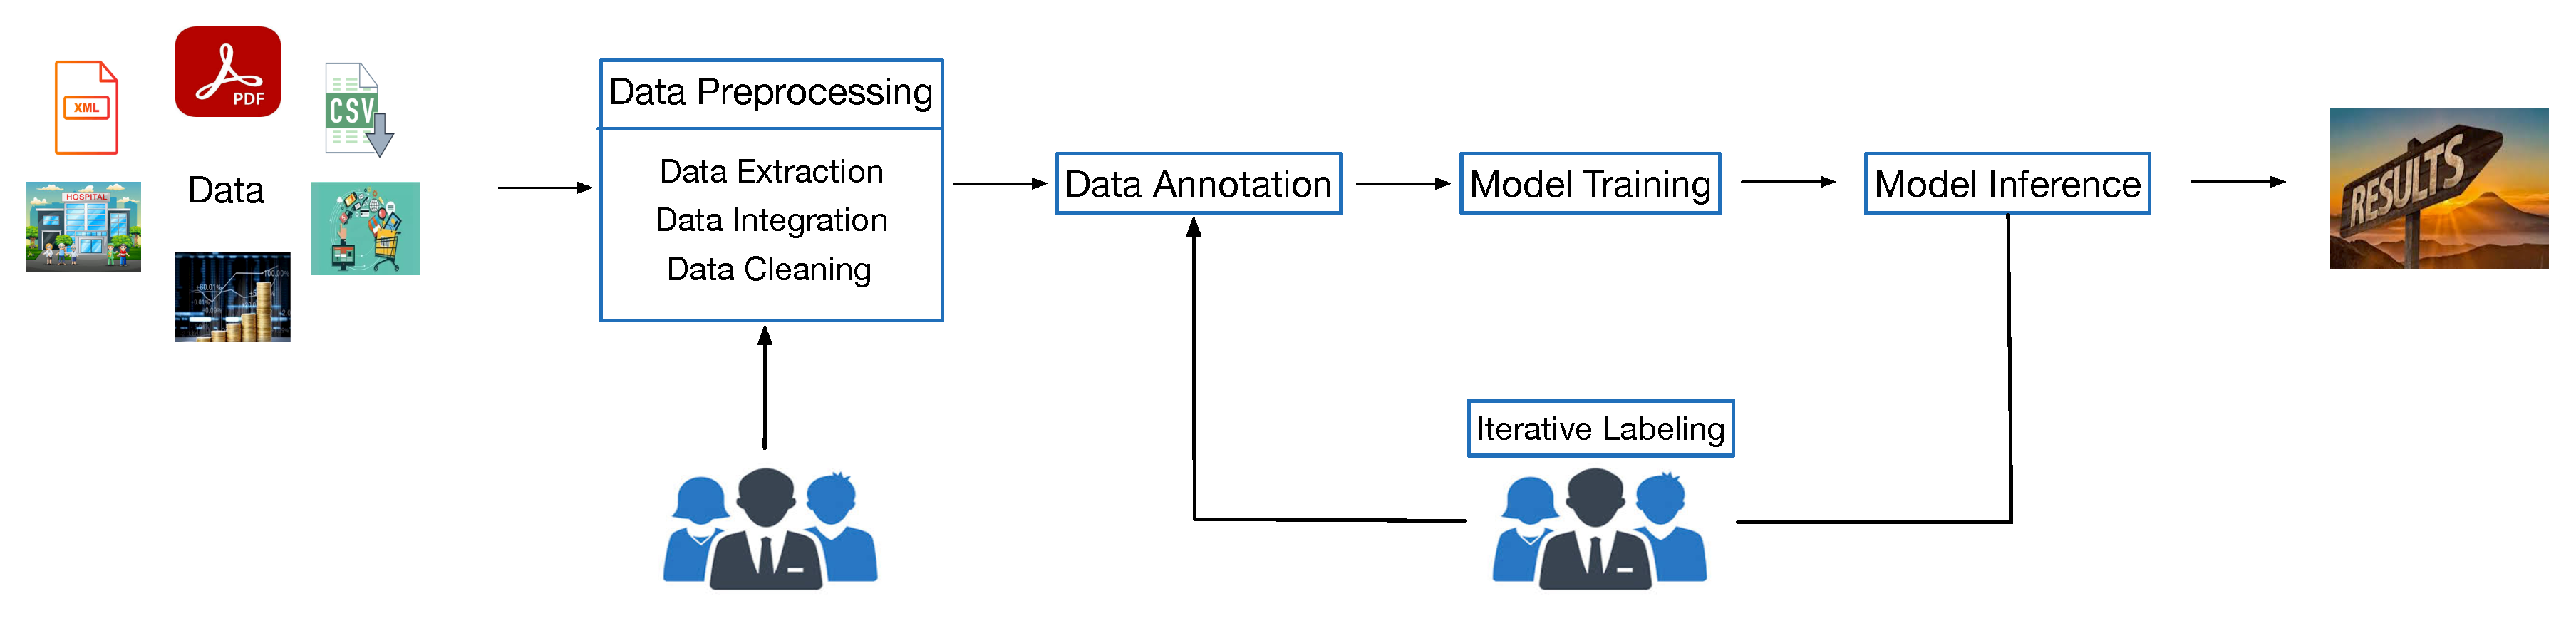
\includegraphics[width=0.65\textwidth]{
%NSFcore-2023/framework.pdf}
 %%\caption{Proposed Project}\label{project}
%\end{wrapfigure}



%We intend to propose complete, partial (either order or unordered), and various qualitative individual preference elicitation models.  An example of the first two would be having complete or only top-$k$ order of preferences over the candidates as inputs, whereas, an example of the last one  would be to bucketize candidates in different qualitative groups (recall the motivating example). For fairness, our effort would be to design group based fairness criteria designed over the protected attributes of the candidates that resemble group fairness criteria, such as, demographic parity, or statistical parity, studied in the context of classification~\cite{verma2018fairness}. To that end, we will adapt proportionate-fairness or p-fairness~\cite{pfair,chairman}  from resource allocation theory that ensures proportionate representation of every group based on a protected attribute in every position of the produced results, or its generalization~\cite{amer2009group} adapted from the social choice theory to promote affirmative action~\cite{fu2006theory} in the produced results.  
%Preference aggregation would be studied considering Kendall-Tau and Spearman's Footrule Distance functions~\cite{kemeny,diaconis1977spearman}, with the objective to minimize the sum of disagreement (Kemeny Optimization) or such, akin to existing {\em (fairness unaware) classical rank aggregation problem}~\cite{dwork2001rank,ailon2008aggregating, ailon2010aggregation}. Our goal would be to make these solutions fairness aware by investigating how to combine these two somewhat conflicting aspects in a systematic manner. For each of these proposed problem variants, we shall analyze the nature of the problem analytically and design scalable solutions with theoretical guarantees. Finally, we will perform both qualitative and quantitative study to develop actionable interventions by leveraging our proposed framework to promote fairness in two compelling applications: (i) Ranked Choice Voting (RCV)~\cite{rcv1,rcv2}, and (ii) Gender and diversity gap in the Oscars. We intend to fine-tune our proposed models based on these evaluations. 

\noindent {\bf Comparison with Existing Work.}
This contribution builds on our work recent works on fairness~\cite{islam2022satisfying, wei2022rank}, and prior works on preference aggregation~\cite{amer2009group, amer2015group, basu2015group}, studying robustness~\cite{roy2014exploiting}. We acknowledge that the existing popular group based fairness definition, such as, {\em statistical parity}~\cite{dwork2012fairness} is somewhat similar to one of our proposed fairness notion. However, the best adapted version of top-$k$ statistical parity studied in a recent paper~\cite{vldbrank} does not account for proportionate representation in every position of the top-$k$, limiting its applicability.  Studying computational challenges related to computing the margin of victory  has been a focus of recent research~\cite{stv1,stv2, stv3} in the context of electoral voting and related applications. But none of these existing works study the general version of the problem, which is, how to promote additional simple/complex constraints/criteria in the output, which is our primary focus. Other than these prior works, which are  much narrow in scope, we are unaware of any computational work that systematically studies different preference elicitation models, multiple output changing criteria, and preference aggregation combining these two.  

%Section~\ref{related} provides an in-depth comparison between our proposed work and existing work.  
%To the best of our knowledge, we are the first to investigate a generic framework that can minimally update original outcome of preference aggregation to satisfy complex constraints without any assumption on the relationship among the attributes.

%Using the aforementioned example, if $k=12$, existing work~\cite{vldbrank} only ensures p-fairness of the aggregated rank at position $12$, but not for the remaining positions (e.g., 1 to 11). {\em While p-fairness promotes stronger notion of fairness, and our proposed framework adapts to top-$k$ statistical parity, existing work does not adapt to our proposed optimization framework}.

%\smallskip \noindent {\bf Aim 1 - Fair Rank Aggregation.}
%We will begin our study in the context of ranking, which is a commonly used method to prioritize  desirable outcomes among a set of candidates and is an essential step in  many high impact applications. Here the members elicit a {\em complete preference order} over the candidates and the goal is to produce an aggregated ranked order over all candidates or produce top-$k$ results that minimize disagreements  among individual preferences. When fairness is studied, our goal would be to ensure fair representation of the candidates based on their one or more protected attributes (such as, gender, race, etc.) in the ranked order. 
%\smallskip \noindent {\bf Aim 2 - Fair Partial and Qualitative Preference Aggregation.}
%In this aim we shall consider scenarios where either qualitative preferences or partial rankings are elicited from the members. 
%We consider three such preferences: (1) top-$t$ ranking, where the input preference is a ranking of the top-$t$ items (candidates), (2) subset selection, where the input preference is an unordered subset of favorite elements, and (3) bucketing, where the input preference is a partition of the elements into three subsets: the ``yes'' set, ``ambivalent'' set, and the ``no'' set.  In our preliminary work, we consider the selection of council members or a committee of $k$ members from $n$ candidates considering the votes of $m$ judges (voters) ({\em ranked choice voting}~\cite{rank1} could be considered as a popular application of that).  The fairness criterion models affirmative action and includes a lower and upper bound on the number of elected candidates, for each value of the protected attributes(s). We intend to study the design choices of different preference elicitation models considering fairness, formalize the optimization problems and analyze them, and design principled solutions with guarantees.

%The mechanism we focus on to aggregate the top-$k$ rankings is {\em Ranked choice voting (RCV)}, and specifically RCV employing a single transferable vote (STV) system~\cite{rcvdesc}.
%We are going to follow the mechanism used in Cambridge MA to elect its city council. 

%\smallskip \noindent {\bf Aim 3 - Actionable Fair Preference Aggregation.}
%Although the proposed models and algorithms consider 
%fairness in its design, rather than an afterthought, the third aim will delve deeper into fairness considerations of compelling applications and develop actionable interventions. In particular, the third aim will provide a holistic large-scale study over two compelling applications and present actionable interventions to promote fairness. In the first application, we will study fairness in Ranked Choice Voting (RCV)\footnote{\small https://qz.com/1676718/the-pros-and-cons-of-ranked-choice-voting/} considering the data provided by the Cambridge, MA
%City Council Election 2019~\cite{RCV} to analytically answer important questions raised in recent research~\cite{rcv1,rcv2,rcv3, rcv4,rcv5}. 1. Does more choice lead to reduced racially polarized voting? 2. Does ranked choice voting enable minority representation?  Based on the analysis, {\em we will develop actionable interventions by leveraging our proposed framework to mitigate these risks}. We will perform both qualitative and quantitative analysis. For qualitative  analysis, we will recruit experienced workers from Amazon Mechanical Turk (the budget justification provided further details). A similar  study would be conducted to investigate the gender and diversity gap in the Academy of Motion Picture Arts and Sciences decisions by combining it with large scale Movielens~\cite{movielens} data and we will develop actionable recommendation to mitigate the gap. Further evaluation plan considering other datasets is described in Section~\ref{eval}.

%\section{Introduction}
\label{seC:intro}
% Interpretability and nutritional labels, generally

An essential ingredient of successful machine-assisted decision-making, particularly in high-stakes decisions, is interpretability --– allowing humans to understand, trust and, if necessary, contest, the computational process and its outcomes.   These decision-making processes are typically complex:  carried out in multiple steps, employing models with many hidden assumptions, and relying on datasets that are often repurposed --- used outside of the original context for which they were intended.\footnote{See Section 1.4 of Salganik's ``Bit by Bit''~\cite{salganik} for a discussion of data repurposing in the Digital Age, which he aptly describes as "mixing readymades with custommades.''}  In response, humans need to be able to determine the ``fitness for use'' of a given model or dataset, and to assess the methodology that was used to produce it.  

To address this need, we propose to develop interpretability and transparency tools based on the concept of a {\em nutritional label}, drawing an analogy to the food industry, where simple, standard labels convey information about the ingredients and production processes. Short of setting up a chemistry lab, the consumer would otherwise have no access to this information. Similarly, consumers of data products cannot be expected to reproduce the computational procedures just to understand fitness for their use.   Nutritional labels, in contrast, are designed to support specific decisions by the consumer rather than completeness of information.  A number of proposals for hand-designed nutritional labels for data, methods, or both have been suggested in the literature\cite{DBLP:journals/corr/abs-1803-09010,DBLP:journals/corr/abs-1805-03677,DBLP:conf/fat/MitchellWZBVHSR19}; we advocate deriving such labels automatically or semi-automatically as a side effect of the computational process itself, embodying the paradigm of {\em interpretability-by-design}. 

Interpretability means different things to different stakeholders, including individuals being affected by decisions, individuals making decisions with the help of machines, policy makers, regulators, auditors, vendors, data scientists who develop and deploy the systems, and members of the general public.  Designers of nutritional labels must therefore consider {\em what} they are explaining,  {\em to whom}, and {\em for what purpose}.  In the remainder of this section, we will briefly describe two regulatory frameworks that mandate interpretability of data collection and processing to members of the general public, auditors, and regulators,  where nutritional labels offer a compelling solution (Section~\ref{sec:intro:reg}).  We then discuss interpretability requirements in data sharing, particularly when data is altered to protect privacy or mitigate bias (Section~\ref{sec:intro:synth}).

\subsection{Regulatory Requirements for Interpretability}
\label{sec:intro:reg}

The European Union recently enacted a sweeping regulatory framework known as the General Data Protection Regulation, or the GDPR~\cite{gdpr}.  The regulation was adopted in April 2016, and became enforceable about two years later, on May 25, 2018.  The GDPR aims to protect the rights and freedoms of natural persons with regard to how their personal data is processed, moved, and exchanged (Article 1).  The GDPR is broad in scope, and applies to ``the processing of personal data wholly or partly by automated means'' (Article 2), both in the private sector and in the public sector.  Personal data is broadly construed, and refers to any information relating to an identified or identifiable natural person, called the {\em data subject} (Article 4).  

According to Article 4, lawful processing of data is predicated on the data subject's {\em informed consent}, stating whether their personal data can be used, and for what purpose (Articles 6, 7).
Further,  data subjects have {\em the right to be informed} about the collection and use of their data.~\footnote{\url{https://gdpr-info.eu/issues/right-to-be-informed/}}
Providing insight to data subjects about the collection and use of their data requires technical methods  that support interpretability.  

Regulatory frameworks that mandate interpretability are also starting to emerge in the US.  New York City was the first US municipality to pass a law (Local Law 49 of 2018)~\cite{Vacca}, requiring that a task force be put in place to survey the current use of ``automated decision systems'' (ADS) in city agencies. ADS are defined as ``computerized implementations of algorithms, including those derived from machine learning or other data processing or artificial intelligence techniques, which are used to make or assist in making decisions.''   The task force is developing recommendations for enacting algorithmic transparency by the agencies, and will propose procedures for: (i) requesting and receiving an explanation of an algorithmic decision affecting an individual (Section 3 (b) of Local Law 49); (ii) interrogating ADS for bias and discrimination against members of legally protected groups, and addressing instances in which a person is harmed based on membership in such groups (Sections 3 (c) and (d)); (iii) and assessing how ADS function and are used, and archiving the systems together with the data they use (Sections 3 (e) and (f)).

Other government entities in the US are following suit.  Vermont is convening an Artificial Intelligence Task Force to ``... make recommendations on the responsible growth of Vermont’s emerging technology markets, the use of artificial intelligence in State government, and State regulation of the artificial intelligence field.''~\cite{Vermont}.  Idaho’s legislature has passed a law that eliminates trade secret protections for algorithmic systems used in criminal justice~\cite{Idaho}.  In early April 2019, Senators Booker and Wyden introduced the Algorithmic Accountability Act of 2019 to the US Congress~\cite{BookerWydenClarke}. The Act, if passed, would use ``automated decision systems impact assessment'' to address and remedy harms caused by algorithmic systems to federally protected classes of people. The act empowers the Federal Trade Commission to issue regulations requiring larger companies to conduct impact assessments of their algorithmic systems.

The use of nutritional labels in response to these and similar regulatory requirements can benefit a variety of stakeholders.  The designer of a data-driven algorithmic method may use them to validate assumptions, check legal compliance, and tune parameters.  Government agencies may exchange labels to coordinate service delivery, for example when working to address the opioid epidemic, where  at least three sectors must coordinate: health care, criminal justice, and emergency housing, implying a global optimization problem to assign resources to patients effectively, fairly and transparently. The general public may review labels to hold agencies accountable to their commitment to equitable resource distribution. 


\subsection{Interpretability with Semi-synthetic Data}
\label{sec:intro:synth}

%Datasets are now increasingly used to train models to make decisions once made by humans.  In these automated systems, biases in the data are propagated and amplified with no human in the loop.  The bias, and the effect of the bias on the quality of decisions made, is not easily detectable due to the relative opacity of the system.  

A central issue in machine-assisted decision-making is its reliance on historical data, which often embeds results of historical discrimination, also known as {\em structural bias}.   As we have seen time and time again, models trained on data will appear to work well, but will silently and dangerously reinforce discrimination~\cite{propublicaJ,amazon_hiring,amazon_delivery}.  Worse yet, these models will legitimize the bias --- ``the computer said so.''  Nutritional labels for data and models are designed specifically to mitigate the harms implied by these scenarios, in contrast to the more general concept of ``data about data.''

Good datasets drive research: they inform new methods, focus attention on important problems, promote a culture of reproducibility, and facilitate communication across discipline boundaries.  But research-ready datasets are scarce due to the high potential for misuse. Researchers, analysts, and practitioners therefore too often find themselves compelled to use the data they have on hand rather than the data they would (or should) like to use.  For example, aggregate usage patterns of ride hailing services may overestimate demand in early-adopter (\ie wealthy) neighborhoods, creating a feedback loop that reduces service in poorer neighborhoods, which in turn reduces usage.  In this example, and in many others, there is a need to alter the input dataset to achieve specific properties in the output, while preserving all other relevant properties.  We refer to such altered datasets as \textit{semi-synthetic}.

Recent examples of methods that produce semi-synthetic data include database repair for causal fairness~\cite{DBLP:conf/sigmod/SalimiRHS19}, database augmentation for coverage enhancement~\cite{DBLP:conf/icde/AsudehJJ19}, and privacy-preserving and bias-correcting data release~\cite{DBLP:conf/ssdbm/PingSH17,DBLP:conf/vldb/RodriguezSPSH18}. A semi-synthetic datasets may be altered in different ways.  Noise may be added to it to protect privacy, or statistical bias may be removed or deliberately introduced.  When a dataset of this kind is released, its composition and the process by which it was derived must be made interpretable to a data scientist, helping determine fitness for use.  For example, datasets repaired for racial bias are unsuitable for studying discrimination mitigation methods, while datasets with bias deliberately introduced are less appropriate for research unrelated to fairness.   This gives another compelling use case for nutritional labels.

%To make our discussion more concrete, let us consider data scientists who must identify datasets appropriate for their task.  This is particularly important when semi-synthetic datasets are being released, to which noise is added to protect privacy, or statistical bias is removed or deliberately introduced.  For example, datasets repaired for racial bias are unsuitable for studying discrimination mitigation methods, while datasets with bias deliberately introduced are less appropriate for research unrelated to fairness.  



%\input{IEEE-data-engineering-IC1/preliminary}
\vspace{-0.2in}
\section{Formalism}\label{preliminary}
\vspace{-0.1in}
%The proposed work aims at developing an optimization guided computational framework that modifies an output obtained from a preference aggregation method applied on a preference elicitation model to produce a modified output that satisfies given criteria. The proposed work aims at developing this framework for a suite of preference elicitation models and preference aggregation methods.
%that satisfies with criteria that guides the need to change the original output minimally while producing a complete or top-$k$ (ordered or unordered) result aggregating individual preferences.

There are $4$ types of inputs that our proposed framework takes: (a)~a set $N$ of $n$ items, where each item has a set $\mathcal{A}$ of discrete attributes.  Each attribute $a\in \mathcal{A}$ has $\ell_a$ different values. (b)~a set of $m$ users, where the $i$-th user $u(i)$ provides her preference as $\sigma_i$. The users' preferences could be rank based, partial or full order, or non rank based. (c)~a distance function $\mathcal{F}$ (defined formally below) that measure the ``distance'' between a set of $m$ input preferences  $\sigma_1, \sigma_2,\ldots, \sigma_m$ and an output $\sigma$ with the required output form. The exact distance function depends on the underlying preference elicitation model and the required output form which may be either a complete ranking of the items or a subset of $k$ items, either ranked or not. (d)~a set $\mathcal{C}$ of output criteria/constraints. Some variants of our problem also include as input a budgetary constraint $B$.

%The proposed work aims at developing an optimization guided computational framework that suitably combines a suite of preference elicitation models with criteria that guides the need to change the original output minimally while producing a complete or top-$k$ (ordered or unordered) result aggregating individual preferences. %Next, we present some definitions that will be used throughout the proposal.  

\begin{definition}\label{def4}
\vspace{-0.1in}
{\bf Distance function $\mathcal{F}$.} Given $m$ input preferences  $\sigma_1, \sigma_2,\ldots, \sigma_m$ and an output $\sigma$ with the required output form, the function $\mathcal{F}(\sigma, \sigma_1, \sigma_2,\ldots, \sigma_m)$ is the distance of $\sigma$ from the input preferences  $\sigma_1, \sigma_2,\ldots, \sigma_m$.
In some cases the function $\mathcal{F}(\cdot)$ is an aggregation of a distance function between a single input preference and the output. Examples for such an aggregation are the sum of the pairwise distances and the maximum distance to any of the input preferences. In other cases $\mathcal{F}(\cdot)$ measures the minimum modification of the input preferences that would result in the preference aggregation method outputting the output $\sigma$. 
%$\mathcal{F}(\sigma, [\sigma_1, \sigma_2,\ldots, \sigma_m])$
\end{definition}

\vspace{-0.1in}
\begin{definition}\label{def1}
\vspace{-0.1in}
{\bf Output criteria/constraints.}  For an attribute $a\in \mathcal{A}$,  let $c(p_a)$ denote the cardinality constraints of items with value $p_a$ ($p_a$ is one of the $\ell_a$ possible values of attribute $a$). Given to the framework is a set $C$ of such cardinality constraints for each attribute value $p_a$, for every $a \in A$, $A \subset \mathcal{A}$. There are two explicit cases that we consider.
\begin{itemize}
    \item {\bf The output $\sigma$ is ordered and consists of $k\le n$ items.} 
    In this case the cardinality constraints are defined for every $\kappa \in [1..k]$ items, and for every  such $\kappa \in [1..k]$, the $\kappa$ top ranked items of output $\sigma$ have to satisfy these cardinality constraints.  
    %the $k$ top ranked items satisfy all cardinality constraints defined over $v$, i.e., it satisfies $c(p^v_{a_1}) \text{ AND } c(p^v_{a_2}) \text{ AND } \ldots \text{ AND } c(p^v_{a_A})$.  
     \item {\bf The output $\sigma$ is an unordered set of $k$ items.} In this case the cardinality constraints are defined for $k$ items and the items in the output set $\sigma$ have to satisfy these cardinality constraints. 
     \\ %$c(p_{a_1}) \text{ AND } c(p_{a_2}) \text{ AND }  \ldots \text{ AND } c(p_{a_A})$.  
\end{itemize}  
\end{definition}
\vspace{-0.1in}
\begin{definition}\label{def3}
\vspace{-0.1in}
{\bf A budgetary constraint.} A budgetary constraint $B$ is an upper bound on the distance of the output from the input preferences. 
%For a given distance function $\mathcal{F}(\cdot)$, 
The budgetary constraint implies that $\mathcal{F}(\sigma,\sigma_1,\sigma_2,\ldots,\sigma_m)\leq B$.  
\end{definition}

\vspace{-0.1in}
\begin{definition}\label{def2}
{\bf Preference Aggregation Considering Constraints.} 
We intend to study different types of problem definitions that require different algorithmic treatments.
Given either complete or partial preferences $\sigma_1,\sigma_2,\ldots,\sigma_m$ over the items in $N$, a preference aggregation method, a distance function $\mathcal{F}(\cdot)$, and a set of output criteria $\mathcal{C}$.
\vspace{-0.1in}
\begin{itemize}
    \item {\bf (Constrained optimization).} Produce an output $\sigma$ with the required form that minimizes $\mathcal{F}(\sigma,\sigma_1,\sigma_2,\ldots,\sigma_m)$ and satisfies $\mathcal{C}$.
    \vspace{-0.1in}
    \item {\bf (Optimization under budgetary constraints).} Produce an output $\sigma$ with the required form that optimizes $\mathcal{C}$,  while satisfying $\mathcal{F}(\sigma,\sigma_1,\sigma_2,\ldots,\sigma_m) \leq B$. (The objective function for optimizing $\mathcal{C}$ varies.)
    \vspace{-0.1in}
    \item {\bf (Bi-criteria optimization).} Given parameters $\alpha$ and $\beta$ produce an output $\sigma$ with the required form that satisfies both $\mathcal{F}(\sigma,\sigma_1,\ldots,\sigma_m) \le \alpha$ and $\mathcal{G}(\mathcal{C}) \le \beta$, where $\mathcal{G}$ is the objective function for optimizing $\mathcal{C}$.
\end{itemize}
\end{definition}
%The individual research aims will describe the various forms of preference elicitation from users and the details of the preference aggregation methods. We first delineate the need to change original output and the challenges that arise from there.
\vspace{-0.1in}
\subsection{Specifying Output Criteria}
We discuss orthogonal reasons where the original outputs coming out of the preference aggregation methods need to be ``massaged'' further. What unifies them is that these criteria are defined over one or more attributes of the items. Depending on how many attributes are involved in the definition and their relationship thereof gives rise to additional challenges.


%\vspace{-0.1in}
%\subsection{Important Concepts and Definitions}\label{pre}
%\vspace{-0.1in}
%\noindent \textbf{Database.} contains $n$ items or candidates. These two terms will be used interchangeably. The set of items will be denoted $V$, individual items will be denoted by $u$ and $v$. \\
%\noindent {\em \bf Individual preference Elicitation:} We consider the following individual preference elicitation models. \\
%\noindent (1) Complete preference: Each of the $4$ members (Judges) may provide a {\em complete order of preference} over the $12$ candidates (Refer to Table~\ref{tab:example_original_rank}). \\
%\noindent (2) Partial preference: 
%(2.1) Ordered. Member 1 (as well as other members) may provide a partial order over the first $5$ candidates and does not specify anything for the rest.\\
%(2.2) Unordered. Member 1 (as well as other members) may also specify that she likes the first $5$ candidates without specifying any order among them.\\
%\noindent (3) Qualitative Preference: Contrarily, Member 1 (as well as other members) may provide {\em qualitative preferences}: Molly and Amy are preferred, Abigail, Kim, Lee are acceptable, the remaining ones must not be considered. These are considered to be the inputs to the framework. Please note that 2.2 is a simplified variant of this last preference elicitation model.

%\noindent \textbf{Multiple Preferences.} The input consists $m$ different preference elicitation (based on the individual models described above). Using the motivating example, $m=4$.

\subsubsection{Fair Preference Aggregation}
We will study fairness in the context of group based protected attributes of the candidates. Output criteria/constraints for fairness (refer to Definition~\ref{def1}) are expressed over one or more {\em protected attributes}. Their protected attributes could be expressed over gender, ethnicity, race, or the state the candidates are living in. 

Formally speaking, each item/candidate $v\in N$ has one or more  {\em protected attributes}. When $\ell_a=2$, it is a binary protected attribute; when $\ell_a \geq 2$ it is a multi-valued protected attribute. As an example, race is (usually) a multi-valued protected attribute, and gender is sometimes a binary protected attribute.

%\begin{itemize}
%\item  {\bf p-fairness.} 
\smallskip \noindent \textbf{p-fairness.}
p-fairness has been studied in the context of resource allocation satisfying temporal fairness or proportionate progress~\cite{chairman, pfair}. It was introduced in the classical  {\em Chairman Assignment Problem}~\cite{baayen1964existence, chairman} that studies how to select a chairman of an union every year from a set of  $n$ states such that  that at any time the accumulated number of chairmen from each state is proportional to its weight. 

In the context of ranking, suppose that each of the $n$ ranked items has a {\em protected attribute} $a(\cdot)$ that can take any of $\ell_a$ different values. For $p_a\in [1..\ell_a]$, let $c'(p_a)$ denote the fraction of items with protected attribute value $p_a$, that is, $c'(p_a) = \frac 1n \sum_{i=1}^n \bbone_{a(i)=p_a}$. The goal is to ensure that $c'(p_a)$ fraction (rounded either up or down) of every top $\kappa$ items have protected attribute value $p_a$.
\iffalse
\vspace{-0.1in}
\item {\bf Generalization of p-fairness to promote affirmative action.} Instead of requiring $c'(p_a)$ fraction of every top $\kappa$ items to have protected attribute value $p_a$, we may want that certain values of the protected attribute get higher representation among the elements at the top, more than their overall proportion. Let $P$ be a non-negative doubly stochastic $n \cdot \ell_a$ matrix. The goal is to ensure that $P(\kappa,p_a)$ fractions (rounded either up or down) of the top $\kappa$ items to have value $p_a$, for every $\kappa \in [1..n]$ and $p_a\in [1..\ell_a]$ (if it is feasible).
It is not difficult to note that such a generalized notion can capture affirmative action.
%\end{itemize}
\fi


\subsubsection{Robust Preference Aggregation}
Output criteria/constraints for robustness on the other hand investigates the flip questions: Given either complete or partial preferences $\sigma_1,\sigma_2,\ldots,\sigma_m$ over $n$ items, let $\sigma$ be the output obtained by the preference aggregation method. Given a budget $B$, how to  make $B$ or less changes in the original preferences, such that the outcome is different from $\sigma$? This question is  related to finding the {\em margin} in electoral systems and quantifies how manipulable the underlying aggregation method is. We study this problem under different manipulation models -- addition only, deletion only, or substitution (addition + deletion).

\iffalse
\subsection{Challenges in Handling  Complex Output  Criteria}
In general, the output requirements/constraints are defined over a set $R$ of attributes. When $|R|=1$, as an example, the output requirement is defined on a single attribute (such as race). In a recent work, we demonstrated that for an aggregation method that models plurality voting, the problem of preference aggregation while satisfying output criteria defined by a single attribute is computationally easy. 
However, the nature of the problem changes when two or more attributes are involved in the output criteria. In Section~\ref{aim1} we discuss this more complicated case and refer to our recent work in which we showed evidence that in some cases it is computationally difficult even to find any output with the required form. 
\fi
%When there are two or more different attributes involved in outlining output criteria/constraints (such as certain representation from race and certain representation from gender), the PIs have proved in a recent work~\cite{islam2022satisfying} that the decision version of the preference aggregation problem under output constraint becomes (weakly) NP-hard by reducing the well known NP-hard Partition problem to our problem~\cite{garey1979computers}. We note that the existing practice of converting multiple attributes to a single multi-valued protected attribute by computing joint distribution over the attributes assumes independence among the attributes. When Independence among the attributes does not hold, this simplification leads to a heuristic process.  The PIs have also demonstrated that for three (or more) attributes (e.g., constraints defined over race, and gender, and ethnicity), even the question whether there exists a set of top-$k$ that satisfies the complex constraint is strongly NP-Hard where the reduction is fro 3 Dimensional Matching. On the positive side for the case of two  attributes, the PIs have designed an efficient algorithm a preference aggregation algorithm while satisfying fairness constraints defined over $2$ attributes and has designed a 2 approximation factor and runs in $O(n^2\ell \log m)$ time, by casting this problem as a min cost flow problem, where $\ell$ is the total number of possible attribute values. We intend to study these aspects in the proposal - as it turns out to be an intellectually demanding and independent  facet of the computational problem, irrespective of the specific reasons to change the output.


%\input{IEEE-data-engineering-IC1/aim1}
\vspace{-0.2in}
\section{Single Round Rank based Preference Aggregation}\label{aim1}
\vspace{-0.1in}
We outline two separate lines of algorithmic problems: (1) incorporating output criteria (e.g., p-fairness) in single round rank-based preference aggregation methods, and (2) satisfying complex constraints in single round rank-based preference aggregation methods.
\vspace{-0.1in}
\subsection{Incorporating output criteria in rank aggregation} 
\vspace{-0.1in}
The input to the classical {\em rank aggregation} problem consists of $m$ complete order of preferences over the $n$ items/candidates. Traditionally, producing the final ranking involves aggregating potentially conflicting preferences from multiple individuals, and is known as the rank aggregation problem~\cite{dwork2001rank,van2007deterministic, ailon2008aggregating}. Our goal is to  minimally change the aggregated output to enable fairness.
%p-fairness has been studied in the theory community to enable resource allocation satisfying temporal fairness or proportionate progress.
We will study p-fairness~\cite{chairman, pfair} that ensures proportionate representation of every group based on a protected attribute in every position of the aggregated ranked order.  The classical problem in this context is known as the {\em Chairman Assignment Problem}~\cite{baayen1964existence, chairman} which studies how to select a chairman of a union every year from a set of  $r$ states such that  that at any time the accumulated number of chairmen from each state is proportional to its weight. p-fairness generalizes other notions of fairness~\cite{islam2023equitable} that were considered in prior work, including the existing popular group based fairness definition {\em statistical parity}~\cite{dwork2012fairness}. 
%We start with some definitions and then describe both our preliminary research and the open problems we plan to investigate further.
\vspace{-0.1in}
\subsubsection{Research Directions}
\vspace{-0.1in}
%\noindent \textbf{Rank and Multiple Ranking.}  
Consider rankings of the items in a set $V$. Each such ranking can be viewed as a permutation. We will use the terms ranking and permutation interchangeably. 

\noindent \textbf{Kendall-Tau and Kemeny distances.}
	Given two rankings $\sigma,\eta: V \rightarrow [1..n]$, the
	Kendall-Tau distance between the two rankings is the sum of pairwise disagreements between $\sigma$ and $\eta$ (bubble-sort distance)
	\[
	\cK (\sigma,\eta) = \sum_{\{u,v\}\subseteq V} \bbone_{(\sigma(v)-\sigma(u))(\eta(v)-\eta(u))<0}.
	\]
	
	For a set of rankings
	$\{\eta_1,\eta_2,\ldots,\eta_m\}$ the {\em Kemeny distance} of the ranking
	$\sigma$ to this set as
	\[
	\kappa(\sigma,\eta_1,\eta_2,\ldots,\eta_m)= \sum_{i=1}^m \cK (\sigma,\eta_i).
	\]

 \noindent \textbf{Spearman's footrule distance.}
    Given two rankings $\sigma,\eta: V \rightarrow [1..n]$, the 	Spearman's footrule distance between the two rankings is the sum of the absolute values
  ($\ell_1$ distance) of the differences between rankings $\sigma$ and $\eta$.
	\[
	\cS (\sigma,\eta) = \sum_{u\in V} |(\sigma(u)-\eta(u)|
	\]
 
	For a set of rankings
	$\{\eta_1,\eta_2,\ldots,\eta_m\}$ the {\em Spearman's footrule distance} of the ranking
	$\sigma$ to this set is the sum of the pairwise distances.

    \noindent \textbf{Rank aggregation.} The aggregated ranking of a set of $m$ rankings $\{\rho_1,\rho_2,\ldots,\rho_m\}$ for a given distance function is a ranking that minimizes  the distance to this set.
    
    \noindent \textbf{p-fairness for a ranking.}
    For a permutation $\sigma, k\in [1..n], p\in [1..\ell]$, let $P(\sigma,k,p)$ denote
    the number of elements with protected attribute value $p$ among the $k$ top ranked elements
    in $\sigma$. A ranking $\sigma$ is {\em proportionate fair} or {\em p-fair} if
    \[
    \forall k\in [1..n]\, \forall p\in [1..\ell]:\  P(\sigma,k,p)\in \{\floor{f(p)\cdot k},\ceil{f(p)\cdot k}\}.
    \]

 
%We note that the best adapted version of top-$k$ statistical parity studied in a recent paper~\cite{vldbrank} does not account for proportionate representation in every position in the top-$k$ positions, but just to a small number of positions, thus limiting its applicability.
%As a matter of fact it can be shown that the algorithm Fair-ILP presented in~\cite{vldbrank} for the special case of a binary protected attribute in which the frequency of both values is the same may produce a very skewed output. This is because the algorithm Fair-ILP just considers the {\em total number of times} items with one value of protected attribute are ranked above items with the other value. p-fairness is  stronger because it ensures statistical parity for every position in the ranked order and considers, for every $k$, the number of times items in the top-$k$ with one value of protected attribute are ranked above items with the other value. This makes this notion of fairness significantly harder to implement and the existing solutions do not trivially adapt.


We formalized two optimization problems, individual p-fairness or {\bf IPF} and the rank aggregation problem subject to proportionate fairness ({\bf RAPF})  considering binary ($\ell=2$) and multi-valued ($\ell > 2$) protected attributes. These problems and associated algorithmic results could be found in~\cite{wei2022rank}.


\vspace{-0.1in}
\subsubsection{Open Problems}
\vspace{-0.1in}
We plan to investigate the following open problems.

\smallskip \noindent{\bf p-fairest aggregate ranking (PFAR).} 
The PFAR problem is defined as follows. Given a set of $m$ rankings %$\{\rho_1,\rho_2,\ldots,\rho_m\}$ 
choose the ``p-fairest'' ranking among all rankings that minimize the Kemeny distance to this set. 
We need to define ``p-fairest'' ranking or a distance measure to a p-fair ranking.
We propose the following distance measure (using the notations defined above).
For an integer $d \ge 0$, a ranking $\sigma$ is at distance $d$ from a {\em p-fair} ranking if
\[
\forall k\in [1..n]\, \forall p\in [1..\ell]:\  P(\sigma,k,p)\in \{\floor{f(p)\cdot k}-d,\ceil{f(p)\cdot k}+d\}.
\]

\iffalse
Another way to view the distance to a p-fair ranking is by considering the classical {\em p-processor cup game} defined by Liu~\cite{liu1969} that considered the notion of p-fairness in multi processor scheduling. The p-processor cup game (adapted to our case) is a multi-round game with two players, an {\em emptier} and a {\em filler}, that takes place on $\ell$ cups, each filled initially with a fixed amount of water, called {\em buffer}. At the beginning of each round,
the filler adds a total of 1 gallon of water to the cups. The distribution of this 1 gallon to the cups is determined by the filler.
The emptier then selects a single cup (that must have at least 1 gallon of water)
and removes 1 gallon from this cup. The emptier’s goal is to minimize the size of the buffer and the {\em backlog} which is the amount of water (on top of the initial amount) in the fullest cup.

It is easy to see the analogy to p-fairness. Consider a p-fair ranking of $n$ elements each with a protected attribute with $\ell$ possible values. Each cup represents a possible value of the protected attribute. The corresponding game has $n$ rounds. In each round $k\in [1..n]$ the filler
adds $f(p)$ gallons of water to cup $p$, for $p\in [1..\ell]$, and the emptier removes 1 gallon of water from the cup corresponding to the value of the protected attribute of the element ranked $k$.
The existence of a p-fair ranking implies that the emptier can always guarantee that the size of the buffer and the backlog is no more than 1 gallon.
For a ranking that is at distance $d$ from a p-fair ranking, the emptier can guarantee that the size of the buffer and the backlog is no more than $1+d$ gallons.
\fi

We observe that PFAR is also NP-Hard as directly follows from the fact that unconstrained rank aggregation is NP-hard when 
$m\ge 4$~\cite{ailon2008aggregating}. For some fixed $\alpha > 1$, We would like to find an algorithm that finds the p-fairest ranking among all rankings whose Kemeny distance from the set of input rankings is at most $\alpha$ times the minimum such distance. 
%Reasonable values of $\alpha$ to consider are 
%$\frac 85$ and $\frac 43$ since there are efficient $\frac 85$ and $\frac 43$ approximation algorithm for the rank aggregation problem~\cite{ailon2008aggregating}.

\smallskip \noindent {\bf Bi-criteria p-fair rank aggregation (BPFRA).} 
The most general problem that we plan to consider in this context is the bi-criteria optimization problem, that is, for a given pair $(\alpha>1 ,\beta>1)$ and a set of $m$ rankings %$\{\rho_1,\rho_2,\ldots,\rho_m\}$
find a ranking whose Kemeny distance to the set of rankings is at most $\alpha$ times the Kemeny distance of the aggregated rank from the set and its distance from a p-fair ranking is at most $\beta$, if such a ranking exists.

\smallskip \noindent{\bf p-fair rank aggregation with affirmative action.} 
We plan to consider a variant of p-fair rank aggregation that involves ``affirmative action''. This will be modeled by varying the proportion of the values of the protected attribute in the p-fair aggregated rank. For example, consider a binary protected attribute with values A and B each needs to appear the same number of times. Suppose that our goal is to promote the items with attribute value A. In this case we can vary the proportion of A making it higher in the top ranked elements and lower in the lower ranked elements so that overall items with attribute value A will appear the same number of times as items with attribute value B.

\smallskip \noindent{\bf The complexity of individual p-fair ranking (IPF).}  We plan to further investigate the IPF problem for multi valued protected attributes as it is open whether it can be solved accurately in polynomial time. We conjecture that this problem is NP-Hard. %and plan to look for a suitable reduction to prove this conjecture. 
We also plan to look for improved approximation algorithms for this problem.
%We note that the algorithm DetConstSort given in~\cite{kddrank} does not produce closest ranking to a given input ranking.

\smallskip \noindent {\bf Better approximation of rank aggregation subject to p-fairness (RAPF).}
We plan to develop more sophisticated RAPF algorithms with better approximation ratios,  %One approach for designing such algorithms is to apply the pivoting technique presented in~\cite{ailon2008aggregating} for rank aggregation. We also plan 
and to improve the computational aspects of the RAPF problem. This problem can be formulated as an Integer Programming (IP) problem. %and thus the RAPF problem of reasonable size can be solved in practice using an IP solver like Gurobi or CPLEX.
We plan to consider various IP formulations as well as various rounding techniques to accelerate the computation.

\smallskip \noindent{\bf Robust rank aggregation.} It is known that rank aggregation under Kemeny distance is NP-hard. We will explore other aggregation methods, such as Spearman's footrule and Borda, and study how manipulable these rank aggregation methods are -- that is, if only $x\%$ of the preferences are allowed to be changed, how easy it is to change the outcome.
\vspace{-0.1in}
\subsection{Complex Constraints} 
\vspace{-0.1in}
Our goal is to optimize preference substitution to satisfy complex top-$k$ fairness constraints, where the fairness requirement is defined over a set $R$ of protected attributes. One of the objectives we will consider is {\em minimizing the number of single ballot (ranking) substitutions that guarantee fairness in the top-$k$ results.} 
%In voting theory~\cite{cary2011estimating}, the concept of margin of victory (MOV) is designed to measure electoral competitiveness of the candidates. 
In a preliminary work we defined the problem of finding the smallest number of single ballot substitutions to promote a set of $k$ candidates that satisfy fairness requirements defined over a set $R$ of protected attributes to the top-$k$. 
\vspace{-0.1in}
\subsubsection{Research Directions}
\vspace{-0.1in}
We assume that there are $\ell$ protected attributes , denoted $A_1,\dots, A_\ell$. For $i\in [1..\ell]$, attribute $A_i$ has $\ell_i$ possible values, denoted $A[i,j]$, for $j\in [1..\ell_i]$. Each candidate is associated with a specific value from each attribute.
In addition, we are given target quantities $a[i,j]$, for $i\in [1..\ell]$, and  $j\in [1..\ell_i]$, with property that all row marginals sum to $k$. Namely, for every $i\in [1..\ell]$, $\sum_{j=1}^{\ell_i} a[i,j] = k$. A fair outcome should satisfy the fairness  condition that for $i\in [1..\ell]$, and  $j\in [1..\ell_i]$, exactly $a[i,j]$ candidates whose $A_i$ attribute value is $A[i,j]$ are elected. 

\noindent We note that one way to approach this problem is by converting the multiple protected attributes to a single multi-valued protected attribute by computing joint distribution over the attributes assuming their independence. For example, instead of considering two binary valued attributes $A_1$ and $A_2$ we consider a single attribute with 4 possible values and the requirement that the value $i*j$ should appear $a[1,i]\cdot a[2,j]/k$ times, for $i,j\in \{1,2\}$. The shortcomings of this approach are two-fold: First, this approach may yield that the problem is infeasible while there is still a solution without assuming independence. A solution that assumes independence may be inferior (require more substitutions) than a solution that does not assume independence.

\noindent In~\cite{islam2022satisfying}, we showed that the problem of finding the smallest number of single ballot substitutions (original preference) to promote a set of $k$ candidates that satisfy proportionate representation over a single protected attribute is computationally easy for any domain size of the protected attribute. On the other hand the same problem becomes computationally hard if we increase the number of protected attributes. When there are two different protected attributes involved in outlining the fairness requirement, we proved that the decision version of that problem is (weakly) NP-hard, %by reducing the well known NP-hard Partition problem to our problem~\cite{garey1979computers}. 
For three (or more) protected attribute, even the question whether there exists a set of top-$k$ that satisfies the complex fairness constraint is strongly NP-Hard by a reduction from 3 Dimensional Matching. On the positive side for the case of two protected attributes we designed an efficient algorithm that obtains a 2 approximation factor and runs in $O(n^2\ell \log m)$ time, 
%by casting this problem as a min cost flow problem, 
where $\ell$ is the number of possible attribute values. We also designed an exact algorithm with running time $n^c$, where $c$ is the size of the Cartesian product of all the attribute domains.

\vspace{-0.1in}
\subsubsection{Open Problems}
\vspace{-0.1in}
There propose two possible ways to extend these problems.

\smallskip \noindent {\bf Improved approximation ratio in the case of 2 protected attributes.} 
Since  the problem of minimizing the number of single ballot substitutions in the case of 2 attributes is currently proven to be weakly NP-Hard, it may admit a PTAS (Polynomial Time Approximation Scheme). We plan to investigate the existence of a better approximation algorithm. Alternatively, we will try to improve the hardness result and show that this problem is strongly NP-Hard or Max-SNP Complete. 

\smallskip \noindent {\bf Relaxed solutions in the case of 3 or more protected attributes.} 
Clearly, the hardness result of even checking the existence of a solution in case of 3 or more attributes precludes the existence of any approximation algorithm for this case. We plan to design an algorithm that will generate a relaxed set of items/candidates. The relaxation may be in two dimensions: (i) the generated set will be a top-$k$ set of candidates but the fairness requirements will not be fully satisfied for all protected attributes. (ii) the generated set will have size larger than $k$ but it will satisfy the (lower bounds of the) fairness constraints for top $k$. Clearly, the larger the generated set is the easier the problem. We will find the smallest such extended set that guarantees the fairness  constraints imposed by all protected attributes.


%\input{IEEE-data-engineering-IC1/Aim2}
\vspace{-0.1in}
\section{Multi Round Rank based Preference Aggregation}\label{aim2}
\vspace{-0.1in}
We study algorithmic challenges to satisfy  output constraints in multi-round rank based preference aggregation methods, popularly known as ranked choice voting or (RCV)~\cite{irv1}. 
\vspace{-0.1in}
\subsection{Research Directions}
\vspace{-0.1in}
We start by describing the STV (single transferable vote) method~\cite{stv-irv, stv1} that generalizes the IRV method, and selects a set of $k$ items/candidates as the winners. STV is gaining popularity as an electoral system. It is used to elect candidates to the Australian Senate, in all elections in Malta, in most elections in the Republic of Ireland, and in Cambridge, MA. There are also plans to use STV in other USA localities. As mentioned in Section~\ref{preliminary} this method of preference aggregation is also applicable in other settings.

The input to an STV preference aggregation method consists of $m$ either complete or partial rankings of the items/candidates. Suppose that the total number of items/candidates is $n$ out of which $k$ items need to be elected. The preference aggregation process requires a predefined {\em quota}. In most cases this quota is Droop quota~\cite{droop} defined as $\floor{\frac{n}{k+1}}+1$. The aggregation is done in rounds. In each round every item/candidate is associated a {\em tally}. Initially, the tally of every item is the number of rankings in which it is ranked highest. A round starts by considering the items whose tally is at least the quota. These items are elected in non-increasing order of their tally, as long as $k$ items/candidates have not been elected (which always holds for Droop quota). When an item is elected their ``surplus'' (the number by which their tally exceeds the quota) is distributed to the next preferred item in their ranking (that has not been eliminated yet). The exact way this ``surplus'' is allocated varies. In a most cases, this allocation is done either fractionally or by a random selection of the surplus rankings out of all the  rankings in which the elected item is top ranked. This is repeated as long as there are items whose tally is at least the quota (and $k$ items/candidates have not been elected). 
Then, if less than $k$ items/candidates are elected, the item/candidate with the smallest tally is eliminated from all the rankings, and the tallies are updated based on the new rankings. If the number of items/candidates remaining (not elected and not yet eliminated) equals the
number of items/candidates left to be elected, these candidates are elected and the STV process terminates, otherwise the process repeats.

There is evidence that IRV and thus also STV preference aggregation methods are computationally hard to manipulate. It is NP-Hard to decide whether an IRV method can be manipulated even by adding one complete ranking~\cite{stv2}. On the positive side, \cite{blom2016,blom2019,magrino2011} suggested branch and bound algorithms that use Integer Programming to compute the Margin of Victory (MOV) in IRV. 

\iffalse
In our preliminary work, 
we considered the selection of $k$ council members out of $n$ {\em candidates} by $m$ voters or {\em members} with no ranking among the $k$ selected candidates. The fairness criterion %for this scenario is quite straightforward: 
is to maintain the proportion of each value of the protected attributes(s) within the selected candidates as in the whole set of candidates, or its generalization that models affirmative action and includes a lower and upper bound on the number of elected candidates, for each value of the protected attributes(s). %Since sometimes affirmative action is required, we consider a generalization where for each value of the protected attributes(s) we are given a lower and upper bound on the number of candidates with this value who have to be elected to the committee.
The challenge is how to produce a fair (or close to fair) solution that accurately reflects the opinions of the voters.

One obvious way is to elicit preference from the members is to ask each member or voter to vote for (up to) a fixed number $t \in [1..k]$ candidates and choose the $k$ candidates who received the most votes, and satisfy the fairness constraints. A clear shortcoming of this simplistic approach is that some of the elected candidates may receive very little support by the voters. For example, in case each voter casts a vote for a single candidate and one of the candidates is endorsed by, say, $90\%$ of the voters, then the rest of the elected candidates would each be elected by less than $10\%$ of the voters. 

Another option is to ask the voters to rank the candidates and then use p-fair rank aggregation as discussed earlier to identify the top $k$ candidates. This option is also not desirable. First, it requires the voters to rank all candidates. Second, this method has some inherent shortcomings as per the celebrated Arrow's impossibility theorem~\cite{arrow,fishburn1970arrow}. These shortcomings are apparent in the specific rank aggregation method used earlier, as this method satisfies the {\em extended Condorcet criterion}, and thus may give total power to a slim majority, ignoring the opinion of a sizable minority. For example, consider the case of $100$ voters and $26$ candidates among whom 13 candidates need to be elected.
Denote the candidates by the letters $A,\ldots,Z$. Suppose that 51 of the voters rank the candidates in order from $A$ to $Z$ while 49 of the voters rank the candidates in reverse order from $Z$ to $A$. The aggregated rank will be $A,\ldots,Z$, implying that the 13 elected candidates will be $A,\ldots, M$, and none of the candidates preferred by 49 of the voters will be elected.

An alternative option that we explore and is regaining popularity recently is the {\em ranked choice voting (RCV)}~\cite{rank1}, and specifically RCV employing a {\em single transferable vote (STV)} system. An STV-RCV means an electoral system in which voters rank up to a fixed $t \in [1..k]$ candidates and ballots transfer to next‐ranked picks until all seats are filled. Broadly, such systems can facilitate majority winners in single‐seat elections, and majority rule with minority representation in multi‐seat elections. There are numerous mechanisms to determine the winners in an STV-RCV. We follow the mechanism used in Cambridge MA to elect its city council as described below (source~\cite{rcvdesc}).

Once ranked ballots have been collected, winners are determined in rounds that are repeated as long as there are still seats that need to be filled.
Each round is called a {\em count}. 
A {\em quota} is set to $q=\floor{n/(k+1)}+1$. %$q=\floor{\frac{n}{k+1}}+1$.
The process in each count is as follows. 
\begin{itemize}
    \item
    If the number of candidates remaining equals the number of seats left to be filled, then all remaining candidates are elected.
    \item 
    Else if the number of first-place votes for a specific candidate is at least the quota $q$, then this candidate is
    elected. The ``surplus'' first-place votes for this candidate, i.e., all votes over $q$ votes, are
    randomly\footnote{The selection is not actually random in the mechanism used in Cambridge MA}
    selected to be transferred to the next candidate(s), as explained below.
    This process is repeated for all candidates who got at least $q$ first-place votes.
    \item
    Otherwise, the candidate with the least first-place votes is eliminated. All the  of first-place votes for the eliminated candidate are transferred, as explained below.
\end{itemize}

The transfer of votes is done by simply erasing the first-place votes in all ballots in which votes need to be transferred,
and treating the second-place vote as the new first-place (if the second-place candidate has been elected or eliminated already, then the votes are transferred further).

This STV-RCV mechanism has the property that minority votes are reflected in the results. As a matter of fact it is shown in~\cite{rcv4} that if for some integer $k>0$ a coalition of at least $k\cdot q$ voters prefers $k$ candidates over the other candidates, then these candidates are guaranteed to be elected. 
\vspace{-0.1in}
\subsection{Open Problems}
\vspace{-0.1in}
\smallskip \noindent {\bf Fair STV-RCV.}
The goal is to develop a fairness aware STV-RCV, using the fairness criterion defined above that still maintains an adequate representation to coalitions. 

We note that the mechanism described above can be modified to satisfy fairness as follows. %First, define some notations.
For $p\in [1..\ell]$, let $\textsc{Cand}(p)$ be the set of all candidates whose protected attribute has value $p$, and let $Upper(p)$, and $Lower(p)$ be the upper and lower bounds on the number of elected candidates from $\textsc{Cand}(p)$ as dictated by the fairness requirement.
To achieve the fairness criterion each count needs to follow the following rules: 
(i) Whenever the number of currently elected candidates from $\textsc{Cand}(p)$ reaches $Upper(p)$, all the votes for other candidates in $\textsc{Cand}(p)$ are transferred. (ii) For any $p\in [1..\ell]$, if the number of currently elected and remaining candidates from $\textsc{Cand}(p)$ equals $Lower(p)$,
then all the remaining candidates from $\textsc{Cand}(p)$ are elected. 
(iii) Let $P\subseteq [1..\ell]$ be the set of all values $p\in [1..\ell]$ for which the number of currently elected candidates from $\textsc{Cand}(p)$ is strictly less than $Lower(p)$, and let $\bar{P}$ be the complement set. Define $S$ to be the sum the differences between $Lower(p)$ and the number of currently elected candidates from $\textsc{Cand}(p)$, for all values of $p\in P$. If $k$ minus the total number of currently elected candidates equals $S$, then the votes for all the remaining candidates in $\cup_{p\in \bar{P}} \textsc{Cand}(p)$ are transferred. 

Clearly, the coalition property of STV-RCV is not maintained in the fairness aware mechanism. We plan to investigate the trade-off between fairness and the power of coalitions and come up with bi-criteria optimized mechanisms.   

\smallskip \noindent {\bf Fair Unordered Partial Preference Aggregation.}
Next, we consider a scenario where partial rankings are elicited from the members (voters). Specifically, each voter specifies a subset of cardinality at most $t$ of elected candidates. Recall that the classical rank aggregation algorithms  are generalized to handle also ties (see, e.g.~\cite{fagin2004comparing}). 
We view each individual preference as a ranking with ties, where
all candidates in the selected subset are tied and above the candidates not in the subset which are also tied. 
We note that in this case the rank aggregation with ties algorithms will not give power to a slim majority as was the case for a complete order. Consider the scenario defined above of $100$ voters and $26$ candidates, $A,\ldots,Z$, among whom 13 candidates need to be elected.
Assume that 51 of the voters elect the subset $A,\ldots,M$ while 49 of the voters elect the complement subset $N,\ldots,Z$. The aggregated rank will be have 7 candidate from $A,\ldots,M$ and 6 from $N,\ldots,Z$. Thus, giving representation also to the minority.  

%\noindent {\bf Problem 2.2: Design a fairness aware mechanism for subset election.}
It can be shown that computing rank aggregation with ties subject to the fairness constraints defined above is NP-hard by reduction from MAX2SAT problem. Thus we plan to consider the problem of finding an efficient approximation algorithm for this problem. We also plan to consider the bi criteria version of this problem where we allow to relax the fairness constraints if it results in a better rank aggregation.

\smallskip \noindent {\bf Fair  Qualitative Preference Aggregation.}
The third scenario we consider is bucketing, in which each individual preference is a partition of the elements into three subsets: set $Y$ of the liked candidates,
set $A$ of the candidates for which there is no firm preference, and set $N$ of the disliked candidates. One obvious way to handle this case is again to consider it as an instance of rank aggregation with ties where we have all the candidates in $Y$ ranked above the candidates in $A\cup N$, and all the candidates in $A$ ranked above the candidates in $N$. The weakness of this approach is that it does not distinguish sometimes between the disliked candidates and the candidates with no firm preference. Specifically, the case of having $k$ candidates liked by a slim majority of the voters but disliked by the rest would be treated the same way as the case of having $k$ candidates liked by a slim majority of the voters and no firm preference by the rest.
Motivated by this example we propose to consider the {\em controversy} of a candidate $c$ and define it as the number of pairs of voters that have contradicting preference of $c$, i.e., the number of pairs of voters for which $c \in Y$ for one voter and $c\in N$ for the other. We intend to study this variant as an open problem.
\fi 

\smallskip \noindent {\bf Approximating the number of ranking substitutions in multi round methods.} 
We plan to develop approximation algorithms with proven performance for IRV and STV. The first step is to design such an algorithm for the simplest case which is approximating the minimum number of ranking substitutions required to change the outcome of an IRV preference aggregation method when every user is limited to input only two top items. From there we hope to be able to generalize to the IRV problem with no restriction on the ranking size, and eventually to the more general STV.

\smallskip \noindent {\bf Improved computational frameworks for minimizing number of ranking substitutions in multi round methods.} 
As mentioned above most of the existing computational frameworks are based on branch and bound algorithms. We plan to investigate other methods and possibly alternative formulation of the respective Integer Programming model that may result in more efficient computational frameworks.

\smallskip \noindent {\bf Heuristic algorithms for minimizing the number of ranking substitutions in multi round methods.} 
Another way to tackle the complex computational problem of minimizing number of ranking substitutions in multi round methods is designing heuristics for this task, analyzing and benchmarking these heuristics. One approach for designing such a heuristic for the problem of minimizing the number of ranking substitutions in STV to guarantee an elected set of $k$ items with a given requirement on their protected attribute is by first identifying the desired elected set and then computing the number of substitutions required to achieve this set. One way of fixing the desired set is as follows. Run the STV process, and whenever the number of the currently elected items/candidates with a given value of their protected attribute reaches its bound, eliminate all the items/candidates with this value of their protected attribute. A naive implementation of this rule may not even guarantee a feasible solution and thus we also need to add the option of reintroducing items/candidates that were already eliminated. Analyzing such an algorithm is a challenge.



%\input{IEEE-data-engineering-IC1/nonrank}
\vspace{-0.1in}
\section{Non-rank based Preference Aggregation}\label{nonrank}
\vspace{-0.1in}
Our goal is to study preference  models that allow users to elicit their choice not as a ranked order. When the input preferences are not ranked, the output produces a set of $k$ items that best reflects the users preferences. Akin to the previous two sections, our goal is to investigate which preference aggregation methods are suitable for such elicitation models, how to handle output constraints, and understand their computational implications. We identify the following research directions.
\vspace{-0.1in}
\subsection{Research Directions}
\vspace{-0.1in}
We begin by considering simple Boolean preference elicitation models, as``only likes'', ``likes and dislikes'' , or ``only dislikes''. Indeed, such preference elicitation models are realistic in a wide variety of applications, such as providing preferences over products, news articles, movies, songs, social media posts, to name a few.

The simplest form of preference elicitation comes in the following form - each user $u(i)$ provides $\sigma_i$ as preference, which is a Boolean vector of $1$'s and $0$'s over the set of $n$ items, and the underlying application \textit{only objective} is to find a set of $k$-items that are ``most liked'' by all the users. We propose to use Jaccard similarity or overlap similarity~\cite{roy2014exploiting} for measuring similarity (inverse of distance) between two vectors in such cases. Given two vectors $\sigma_i, \sigma_j$ their overlap similarity $S_{\sigma_i, \sigma_j} = \sum_{\forall \ell \in [n]} [\sigma_{i_\ell} \land \sigma_{j_\ell}]$, the number
of positive bits that are shared between $\sigma_i, \sigma_j$. When  the users provide both ``likes'' and ``dislikes'' and both have to be accounted for, we will use Hamming Distance  which measures the minimum number of substitutions required to change $\sigma_i$ to  $\sigma_j$. 

We have explored two alternative preference aggregation methods~\cite{amer2009group, roy2014exploiting} in the past that serve as the basis of this study.
\begin{itemize}
    \item \textbf{Aggregated Voting.} Produce $\sigma$, such that $\mathcal{F}(\sigma,\sigma_1) + \mathcal{F}(\sigma,\sigma_2) +\ldots \mathcal{F}(\sigma,\sigma_m)$ is minimized.
     \item \textbf{Least Misery.} Produce $\sigma$, such that $\mathbf{Maximum}\{\mathcal{F}(\sigma,\sigma_1), \mathcal{F}(\sigma,\sigma_2),\ldots \mathcal{F}(\sigma,\sigma_m)\}$ is minimized.
\end{itemize}
The goal is to produce $\sigma$, which is also a vector of length $n$ with exactly $k$ number of 1's and remaining $0's$ that minimizes the Inverse of overlap similarity/Hamming Distance, denoted $\mathcal{F}(\cdot,\cdot)$, between $\sigma$ and $\{\sigma_1,\sigma_2,....\ldots,\sigma_m\}$.

We realize that the overlap similarity function is monotone, as when a new item is considered in the mix, the overlap similarity can never decrease (or inverse overlap similarity can never increase). This is likely to make preference aggregation computationally tractable and give rise to polynomial time solution to produce optimal $\sigma$. Under Hamming distance, however, finding $\sigma$ considering either of the preference aggregation models is likely to be NP-hard, as a known NP-Complete problem Median String Problem could be reduced to a variant of this problem~\cite{de2000topology}. \\
{\bf Satisfying Output Constraints.}
The output constraints in this case are defined on the top-$k$ items/candidates and involve one or more protected attributes. When the output criteria is simple (designed on a single attribute),  the Preference Aggregation Problems Considering Constraints  defined in Section~\ref{preliminary} for aggregated voting under Overlap Similarity is likely to give rise to computationally tractable problem for all three variants - Constrained optimization, Optimization under budgetary constraints, and Bi-criteria optimization. On the other hand, these problems are likely to be computationally harder for least misery under Overlap Similarity. We will study how to exploit the monotonicity property of overlap similarity to see if it is possible to design greedy algorithms with provable approximation factors. Under Hamming Distance, irrespective of the underlying aggregation method, the Preference Aggregation Problems Considering Constraints are likely to be NP-hard, since the Preference Aggregation under Hamming Distance itself is NP-hard. We intend to study the possibility of designing approximation algorithms as well as efficient heuristics for these problems.
\subsection{Open Problems}
The applicability of the ordinal preference model is explored as one of the open problems - an ordinal value $g$ is defined on an $s$-point performance scale, that is totally ordered  ${g_1 \prec g_2 \prec \ldots \prec g_s}$. Given $m$ input ordinal preferences and an output criteria, goal is to produce $\sigma$ (an ordered list of $n$ items/ top-$k$ ordered/unordered set) that aggregates the preferences and satisfies the criteria. The input is studied as {\em ordered sorting} problem in decision aid literature~\cite{figueira2005choice}. Concretely speaking, each user's preference $\sigma_i$ corresponds to assignment of each item into a pre-defined ordered categories, such as {\em excellent, good, average, poor} and the aggregation problem intends to find the best set of $k$-items $\sigma$. When studied under output constraints, the general challenge is to minimally change the original outcome so as to satisfy the constraints. \\
{\bf Preference Aggregation Methods.}
One key challenge in ordinal preference elicitation model is to identify the appropriate aggregation method and/or distance functions. Per our initial investigation, we realize that an ordinal preference elicitation  could be expressed as a set of pairwise comparisons. As an example, if user $u(i)$ rates $i_1$ as excellent, $i_2$ as good, and $i_3$ as fair, this gives rise to the following $3$ pairwise comparisons: $i_1 \prec i_2, i_2 \prec i_3, i_1 \prec i_3$. 
Given two preferences $\sigma_i, \sigma_j$, one can compute Kendall-Tau distance between these two to quantify the {\em number of inversions} or {\em distance} between them. Given $m$ input preferences  $\sigma_1,\sigma_2,....\ldots,\sigma_m$, when the output is to produce an ordered outcome, the preference aggregation problem intends to produce a ranking $\sigma$ that optimizes (minimizes) the Kemeny Distance~\cite{wei2022rank} (sum of Kendall-Tau distance) between  $\sigma$ and $\{\sigma_1,\sigma_2,\ldots,\sigma_m\}$. 

Additionally, we will study partial net score~\cite{figueira2005choice} of an item $i$ ($PNS(i)$) that is proposed as an indicator of computing the overall ``worth'' of an item in decision aid literature. Based on the aforementioned pairwise representation, $PNS(i)$ can be expressed as 
%\begin{equation*}
    $PNS(i) =  \sum_{j \in [n]\setminus\{i\}} 
    \left(|u^{[i \prec j]}| - |u^{[j \prec i]}|\right)$.
%\end{equation*}
Basically, $PNS(i)$ is the number of times item $i$ is preferred over any other item $j$ by any user (represented as $u^{[i \prec j]}$) minus the number of times these other items are preferred over $i$ by any user (represented as $u^{[j \prec i]}$). By computing partial net score of each item one can design the outcome $\sigma$ easily and efficiently. If $\sigma$ needs to be ordered then the items will be ordered in decreasing order of partial net score; when the goal is to produce a top-$k$ set of items, this will contain the items with the top-$k$ highest partial net score.\\
{\bf Satisfying Output Constraints.}
We will study how to satisfy output constraints that are suitable to ordinal preference models. We will study both simple and complex output constraints, defined over single and multiple attributes, respectively. For the preference aggregation problem under output constraints, this is equivalent to producing a $\sigma$ that minimizes the partial net score or Kemeny Distance between  $\sigma$ and input preferences, while satisfying the output constraints. When studied as an optimization problem under budgetary constraints $B$ ($B$ is the upper bound of partial net score or Kemeny Distance), the goal will be to produce $\sigma$, such that partial net score or Kemeny Distance is at most $B$ and $\mathcal{C}$ is optimized. We anticipate most of these problems to be NP-hard. We will study how to design efficient approximation algorithms with provable guarantees, as well as effective heuristic algorithms.


\vspace{-0.1in}
\section{Conclusion}
\vspace{-0.1in}
The article lays a scientific foundation for systematically changing the outcome of a variety of preference aggregation methods to satisfy additional criteria related to fairness and robustness.  The article studies single-round rank based, multi-round rank based, and non rank based preference aggregation methods that are suitable to different preference elicitation models and investigates how to minimally modify them to promote fairness. It identifies underlying computational and algorithmic challenges, proposes research directions, and formalizes several open problems. 

\vspace{-0.1in}
\section{Acknowledgment}
\vspace{-0.1in}
The work is supported by the NSF CAREER Award \#1942913, IIS \#2007935,
IIS \#1814595, PPoSS:Planning \#2118458, and by the Office of Naval
Research Grants No: \#N000141812838, \#N000142112966.

\vspace{-0.2in}
\bibliographystyle{abbrv}
%\bibliography{BIB/mixed}
\bibliography{paperbib}



\end{document}



\end{article}
\begin{article}
{On the Robustness of ChatGPT: An Adversarial and Out-of-distribution
Perspective}
{Jindong Wang, Xixu Hu, Wenxin Hou, Hao Chen, Runkai Zheng, Yidong Wang, Linyi Yang, Wei Ye, Haojun Huang, Xiubo Geng, Binxing Jiao, Yue Zhang, Xing Xie}
\setcounter{section}{0}
\documentclass[11pt]{article}
\usepackage{deauthor}
\usepackage{times,graphicx}

% user packages
\usepackage{todonotes}
\usepackage{pifont}

\newcommand{\cmark}{\ding{51}}
\newcommand{\xmark}{\ding{55}}
\usepackage{multirow}
\usepackage{booktabs}
\usepackage{caption,subcaption}
\usepackage{graphicx}
\usepackage{xspace}
\usepackage{url}
\usepackage{amsmath,amssymb,amsfonts}
\usepackage{algorithm}
\usepackage{algorithmicx}
\usepackage{algpseudocode}

\usepackage{bbm}
\usepackage{hyperref}       % hyperlinks
\usepackage{url}            % simple URL typesetting
\usepackage{amsmath}
\usepackage{booktabs}       % professional-quality tables
\usepackage{amsfonts}       % blackboard math symbols
\usepackage{nicefrac}       % compact symbols for 1/2, etc.
\usepackage{microtype}      % microtypography
\usepackage{xcolor}         % colors
\usepackage{xspace}
\usepackage{todonotes}
\usepackage{adjustbox}
\usepackage{authblk}    % return to previous author style
\usepackage{cleveref}
\usepackage{makecell}
% \usepackage{subfigure}
\usepackage{subcaption}
\usepackage{multirow}
\usepackage{epsfig}
\usepackage{epstopdf}
\usepackage{bbding}


% \usepackage{ulem}

%%% CUSTOM COMMANDS
\newcommand{\wyd}[1]{{\color{red}{[(WYD): #1]}}}
\newcommand{\wydd}[1]{\todo[linecolor=cyan,backgroundcolor=cyan!25,bordercolor=cyan,size=\scriptsize]{(WYD): #1}}

\newcommand{\wjdd}[1]{\todo[linecolor=cyan,backgroundcolor=cyan!25,bordercolor=cyan,size=\scriptsize]{(WJD): #1}}
\newcommand{\wjd}[1]{{\color{cyan}{[(WJD): #1]}}}
\newcommand{\ch}[1]{{\color{blue}{[(CH): #1]}}}
\newcommand{\hwx}[1]
{\todo[linecolor=purple,backgroundcolor=purple!25,bordercolor=purple,size=\scriptsize]{(HWX): #1}}

\newcommand{\chat}{ChatGPT\xspace}
\newcommand{\advglue}{AdvGLUE\xspace}
\newcommand{\flip}{Flipkart\xspace}
\newcommand{\ddx}{DDXPlus\xspace}
\newcommand{\error}[1]{\textcolor{red}{#1}}

\newcommand{\tabincell}[2]{\begin{tabular}{@{}#1@{}}#2\end{tabular}}

\title{On the Robustness of ChatGPT: An Adversarial and Out-of-distribution Perspective}

% The \author macro works with any number of authors. There are two commands
% used to separate the names and addresses of multiple authors: \And and \AND.
%
% Using \And between authors leaves it to LaTeX to determine where to break the
% lines. Using \AND forces a line break at that point. So, if LaTeX puts 3 of 4
% authors names on the first line, and the last on the second line, try using
% \AND instead of \And before the third author name.



\author{%
  \textbf{Jindong Wang}$^{1}$\thanks{Contact: jindong.wang@microsoft.com.}, \textbf{Xixu Hu}$^{1,2\ddagger}$\thanks{Equal contribution.}, \textbf{Wenxin Hou}$^{3\dagger}$, \textbf{Hao Chen}$^{4}$, \textbf{Runkai Zheng}$^{1,5}$\thanks{Work done during internship at Microsoft Research Asia.}, \\\textbf{Yidong Wang}$^{6}$, \textbf{Linyi Yang}$^{7}$, \textbf{Wei Ye}$^{6}$, \textbf{Haojun Huang}$^{3}$, \textbf{Xiubo Geng}$^{3}$, \\\textbf{Binxing Jiao}$^{3}$, \textbf{Yue Zhang}$^{7}$, \textbf{Xing Xie}$^{1}$\\
  $^{1}$Microsoft Research, $^{2}$City University of Hong Kong, $^{3}$Microsoft STCA, \\$^{4}$Carnegie Mellon University, $^{5}$Chinese University of Hong Kong (Shenzhen), \\$^{6}$Peking University, $^{7}$Westlake University
}

\begin{document}

\maketitle


\begin{abstract}

\chat is receiving increasing attention over the past few months.
While evaluations of various aspects of \chat have been done, its robustness, i.e., the performance to unexpected inputs, is still unclear to the public.
Robustness is of particular concern in responsible AI, especially for safety-critical applications.
In this paper, we conduct a thorough evaluation of the robustness of \chat from the adversarial and out-of-distribution (OOD) perspective.
To do so, we employ the \advglue and ANLI benchmarks to assess adversarial robustness and the Flipkart review and \ddx medical diagnosis datasets for OOD evaluation.
We select several popular foundation models as baselines.
Results show that \chat shows consistent advantages on most adversarial and OOD classification and translation tasks.
However, the absolute performance is far from perfection, which suggests that adversarial and OOD robustness remains a significant threat to foundation models.
% Further synopsis indicates that prompt is pivotal to the performance of \chat and we present two suggestions for prompt design: adding more detailed instructions and incorporating chain-of-thought methods.
Moreover, \chat shows astounding performance in understanding dialogue-related texts and we find that it tends to provide informal suggestions for medical tasks instead of definitive answers.
Finally, we present in-depth discussions of possible research directions.

\end{abstract}

\section{Introduction}
\label{sec-intro}

Large language models (LLMs), or foundation models~\cite{bommasani2021opportunities}, have achieved significant performance on various natural language process (NLP) tasks.
Given their superior in-context learning capability~\cite{min2022rethinking}, prompting foundation models has emerged as a widely adopted paradigm of NLP research and applications.
\chat is a recent chatbot service released by OpenAI~\cite{chatgpt}, which is a variant of the Generative Pre-trained Transformers (GPT) family.
Thanks to its friendly interface and great performance, \chat has attracted over $100$ million users in two months.
% By simply inputting prompts, it can generate answers to various NLP tasks.

It is of imminent importance to evaluate the potential risks behind \chat given its increasing worldwide popularity in diverse applications.
While previous efforts have evaluated various aspects of \chat in law~\cite{choi2023chatgpt}, ethics~\cite{shen2023chatgpt}, education~\cite{khalil2023will}, and reasoning~\cite{bang2023multitask}, we focus on its \emph{robustness}~\cite{bengio2021deep}, which, to our best knowledge, has not been thoroughly evaluated yet.
Robustness refers to the ability to withstand disturbances or external factors that may cause it to malfunction or provide inaccurate results.
It is important to practical applications especially the safety-critical scenarios.
For instance, if we apply \chat or other foundation models to fake news detection, a malicious user might add noise or certain perturbations to the content to bypass the detection system.
Without robustness, the reliability of the system collapses.

Robustness threats exist in a wide range of scenarios: out-of-distribution (OOD) samples~\cite{wang2022generalizing}, adversarial inputs~\cite{goodfellow2014explaining}, long-tailed samples~\cite{zhang2021deep}, noisy inputs~\cite{natarajan2013learning}, and many others.
In this paper, we pay special attention to two popular types of robustness: the adversarial and OOD robustness, both of which are caused through input perturbation.
Specifically, adversarial robustness studies the model's stability to adversarial and imperceptible perturbations, e.g., adding trained noise to an image or changing some keywords of a text.
On the other hand, OOD robustness measures the performance of a model on unseen data from different distributions of the training data, e.g., classifying sketches using a model trained for art painting or analyzing a hotel review using a model trained for appliance review.
More background of these robustness is elaborated in \cref{sec-back-robust}.



\textbf{Zero-shot robustness evaluation.}
While robustness research often requires training and optimization (e.g., fine-tuning, linear probing, domain adaptation and generalization, \cref{sec-back-robust}), in this work, we focus on \emph{zero-shot} robustness evaluation.
Given a foundation model, we perform inference directly on the test dataset for evaluation.
We argue that it becomes more expensive and unaffordable to train, or even load existing (and future, larger) foundation models.
For instance, the largest Flan-T5 model has $11$ billion parameters~\cite{chung2022scaling}, which is already beyond the capability of most researchers and practitioners.
Thus, their zero-shot performance becomes important to downstream tasks.
On the other hand, foundation models are typically trained on huge volumes of datasets with huge amount of parameters, which seems to challenge conventional machine learning theories:
\begin{center}
    \emph{Are large foundation models all we need for robustness?}
\end{center}

\begin{figure}[t!]
    \centering
    \includegraphics[width=\textwidth]{submissions/submission4/figures/model_acc_param.pdf}
    \caption{Robustness evaluation of different foundation models: performance vs. parameter size. Results show that \chat shows consistent advantage on adversarial and OOD classification tasks. However, its absolute performance is far from perfection, indicating much room for improvement.}
    \label{fig-summary}
\end{figure}

In this work, we conduct a thorough evaluation of \chat on its adversarial and OOD robustness for natural language understanding tasks.
It is challenging to select appropriate datasets for evaluating 
 \chat since it is known to be trained on huge text datasets as of 2021.
Eventually, we leverage several recent datasets for our evaluation: \advglue~\cite{wang2021adversarial} and ANLI~\cite{nie2019adversarial} for adversarial robustness and two new datasets for OOD robustness: \flip review~\cite{flipkart_2023} and \ddx medical diagnosis datasets~\cite{tchango2022ddxplus}.
Furthermore, we randomly selected $30$ samples from \advglue to form an adversarial translation dataset to evaluate the translation performance.
These datasets represent various levels of robustness, thus provide a fair evaluation.
The detailed information of these datasets are introduced in \cref{sec-dataset}.
We then select several popular foundation models from Huggingface model hub and OpenAI service\footnote{Huggingface: \url{https://huggingface.co/models}. OpenAI service: \url{https://openai.com/api}.} to compare with \chat.
In summary, we have $9$ tasks and $2,089$ test examples.

\textbf{Our findings.}
We perform zero-shot inference on all tasks using these models and \cref{fig-summary} summarizes our main results.
The major findings of the study include:
\begin{enumerate}
    \item What \chat does well: 
    \begin{itemize}
        \item \chat shows consistent improvements on most adversarial and OOD classification tasks.
        \item \chat is good at translation tasks. Even in the presence of adversarial inputs, it can consistently generate readable and reasonable responses.
        \item \chat is better at understanding dialogue-related texts than other foundation models. This could be attributed to its enhanced ability as a chatbot service, leading to good performance on \ddx dataset.
    \end{itemize}
    
    \item What \chat does not do well:
    \begin{itemize}
        \item The absolute performance of \chat on adversarial and OOD classification tasks is still far from perfection even if it outperforms most of the counterparts.
        \item The translation performance of \chat is worse than its instruction-tuned sibling model text-davinci-003.
        \item \chat does not provide definitive answers for medical-related questions, but instead offers informed suggestions and analysis. Thus, it can serve as a friendly assistant.
    \end{itemize}

    % \item Empirical findings of prompt design:
    % \begin{itemize}
    %     \item Adding more detailed instructions about the task to the prompts leads to better results.
    %     \item Incorporating Chain-of-Thought (CoT)~\cite{kojima2022large} methods improves expalanability.
    % \end{itemize}

    \item Other general findings about foundation models:
    \begin{itemize}
        \item Task-specific fine-tuning helps language models perform better on related tasks, e.g., NLI-fine-tuned RoBERTa-L has similar performance to Flan-T5-L.
        \item Instruction tuning benefits large language models, e.g., Flan-T5-L achieves comparable performance to text-davinci-002 and text-davinci-002 with significantly less parameters.
    \end{itemize}
        
\end{enumerate}

Beyond evaluations, we share more reflections in the discussion and limitation sections, providing experience and suggestions to future research.
Finally, we open-source our code and results at \url{https://github.com/microsoft/robustlearn} to facilitate future explorations.


\section{Background}
\label{sec-back}

\subsection{Foundation Models, \chat, and Existing Evaluation}

Foundation models have become a popular research and application paradigm for natural language process tasks.
Since foundation models are trained on large volumes of data, they show significant performance improvement on different downstream tasks such as sentiment analysis, question answering, automatic diagnosis, logical reasoning, and sequence tagging.
\chat is a generative foundation model that belongs to the GPT-3.5 series in OpenAI's GPT family, coming after GPT~\cite{radford2018improving}, GPT-2~\cite{radford2019language}, GPT-3~\cite{brown2020language}, and InstructGPT~\cite{ouyang2022training}.
In contrast to its predecessors, \chat makes it easy for every one to use just through a browser with enhanced multi-turn dialogue capabilities.
Although the technical details of \chat is still not released, it is known to be trained using reinforcement learning from human feedback (RLHF)~\cite{christiano2017deep} with instruction tuning.
Other than natural language processing, there are also emerging efforts in building foundation models for computer vision~\cite{dehghani2023scaling}, music generation~\cite{agostinelli2023musiclm}, biology~\cite{luo2022biogpt,lee2020biobert}, and speech recognition~\cite{radford2022robust}.

Previous efforts evaluate \chat in different aspects~\cite{van2023chatgpt}.
\cite{bang2023multitask} proposes a multi-task, multi-modal, and multilingual evaluation of \chat on different tasks.
They showed that \chat performs reasonably well on most tasks, while it does not bring great performance on low-resource tasks.
Similar empirical evaluations are also made by \cite{gozalo2023chatgpt,azaria2022chatgpt}.
Specifically, \cite{qin2023chatgpt} also did several evaluations and they found that \chat does not do well on fine-grained downstream tasks such as sequence tagging.
In addition to research from artificial intelligence, researchers from other areas also showed interest in \chat.
\cite{hacker2023regulating,shen2023chatgpt} expressed concerns that \chat and other large models should be regulated since they are double-edged swords.
The evaluations on ethics are done in \cite{zhuo2023exploring}.
There are reflections and discussions from law~\cite{choi2023chatgpt}, education~\cite{khalil2023will,m2022exploring,susnjak2022chatgpt,guo2023close}, human-computer interaction~\cite{tabone2023using}, medicine~\cite{jeblick2022chatgpt}, and writing~\cite{biswas2023chatgpt}.
To the best of our knowledge, a thorough robustness evaluation is currently under-explored.


\subsection{Robustness}
\label{sec-back-robust}


In the following, we present the formulation of robustness with the classification task (other tasks can be formulated similarly).
We are given a $K$-class classification dataset $\mathcal{D}=\{\mathbf{x}_i, y_i\}_{i=1}^n$, where $\mathbf{x} \in \mathbb{R}^d$ and $y \in [K]$ are its $d$-dimensional input and output, respectively.
We use $\ell[\cdot, \cdot]$ to denote the loss function.

\paragraph{Adversarial robustness}
An adversarial input~\cite{goodfellow2014explaining} $\mathbf{x}^\prime$ is generated by adding a $\epsilon$-bounded, imperceptible perturbation $\delta$ to the original input $\mathbf{x}$.
The optimal classifier can be learned by optimizing the following objective~\cite{madry2017towards}:
\begin{equation*}
    \min_{f \in \mathcal{H}} \mathbb{E}_{(\mathbf{x}, y) \in \mathcal{D}} \max_{|\delta| \le \epsilon} \ell [f(\mathbf{x} + \delta), y].
\end{equation*}

\paragraph{Out-of-distribution robustness}
On the other hand, OOD robustness (generalization)~\cite{wang2022generalizing,shen2021towards} aims to learn an optimal classifier on an unseen distribution by training on existing data.
One popular formulation for OOD robustness is to minimize the average risk on all distributions $e$, which is sampled over the set of all possible distributions (could be large than $\mathcal{D}$):
\begin{equation*}
    \min_{f \in \mathcal{H}} \mathbb{E}_{e \sim \mathcal{Q}} \mathbb{E}_{(\mathbf{x}, y) \in \mathcal{D}^e} \ell[f(\mathbf{x}), y].
\end{equation*}

\cite{yang2022glue} presented GLUE-X, a benchmark based on GLUE and then conducted a thorough evaluation of the OOD robustness of language models by training on in-distribution (ID) sets and then testing on OOD sets.
Ours, however, performs zero-shot evaluation.
The OOD robustness of \chat cannot be evaluated by GLUE and GLUE-X benchmarks since it may include the entire GLUE datasets in its training data.

\section{Datasets and Tasks}
\label{sec-dataset}

\subsection{Adversarial Datasets}

We adopt \advglue~\cite{wang2021adversarial} and adversarial natural language inference (ANLI)~\cite{nie2019adversarial} benchmarks for evaluating adversarial robustness.
\advglue is a modified version of the existing GLUE benchmark~\cite{wang2019glue} by adding different kinds of adversarial noise to the text: word-level perturbation (typo), sentence-level perturbation (distraction), and human-crafted perturbations.
We adopt $5$ tasks from \advglue: SST-2, QQP, MNLI, QNLI, and RTE.
Since the test set of \advglue is not public, we adopt its development set instead for evaluation.
Although \advglue is a classification benchmark, we additionally construct an adversarial machine translation (En $\to$ Zh) dataset,  termed \advglue-T, by randomly selecting $30$ samples from \advglue. 

ANLI is a large-scale dataset designed to assess the generalization and robustness of natural language inference (NLI) models, which was created by Facebook AI Research. It comprises 16,000 premise-hypothesis pairs that are classified into three categories: entailment, contradiction, and neutral. The dataset is divided into three parts (R1, R2, and R3) based on the number of iterations used during its creation, with R3 being the most difficult and diverse.
Therefore, we select the test set of R3 for evaluating the adversarial robustness of our models.
% Detailed information of \advglue and ANLI can be found in \cref{append-data-adv}.

\begin{table}[t!]
\caption{Statistics of test sets in this paper}
\label{tb-dataset}
\centering
% \resizebox{\textwidth}{!}{
\begin{tabular}{ccccc}
\toprule
Area & Dataset & Task & \#Sample & \#Class \\ \midrule
\multirow{7}{*}{\begin{tabular}[c]{@{}c@{}}Adversarial   \\ robustness\end{tabular}} & SST-2 & sentiment classification & 148 & 2 \\ 
 & QQP & quora question pairs & 78 & 3 \\ 
 & MNLI & multi-genre natural language inference & 121 & 3 \\ 
 & QNLI & question-answering NLI & 148 & 2 \\ 
 & RTE & textual entailment recognition & 81 & 2 \\ 
 & ANLI & text classification & 1200 & 3 \\
 & \advglue-T & machine translation (En $\to$ Zh) & 30 & - \\ 
 \midrule
\multirow{2}{*}{\begin{tabular}[c]{@{}c@{}}OOD \\ robustness\end{tabular}} & Flipkart & sentiment classification & 331 & 2 \\ 
 & DDXPlus & medical diagnosis classification & 100 & 50 \\ \bottomrule
\end{tabular}
% }
\end{table}


\subsection{Out-of-distribution Datasets}

We adopt two new datasets\footnote{Considering \chat is reported to be trained on a substantial corpus of internet language data as of 2021, identifying an out-of-distribution dataset poses a difficulty. Furthermore, we concern that previous natural language processing datasets predating 2022 may have been assimilated by \chat, so we only utilize datasets that are recently released.} for OOD robustness evaluation: \flip~\cite{flipkart_2023} and \ddx~\cite{tchango2022ddxplus}.
\flip is a product review dataset and \ddx is a new medical diagnosis dataset, both of which are released in 2022.
These two datasets can be used to construct classification tasks.
We randomly sample a subset of each dataset to form the test sets.
% Detailed introduction and construction of each test set can be found in \cref{append-data-ood}.
\cref{tb-dataset} shows the statistics of each dataset.

\emph{Remark:}
Finding an OOD dataset for large models like \chat is difficult due to the unavailability of its training data.
Consider these datasets as `out-of-example' datasets since they did not show up in \chat's training data.
Additionally, distribution shift may happen at different dimensions: not only across domains, but also across time.
Thus, even if \chat and other LLMs may already use similar datasets like medical diagnosis and product review, our selected datasets are still useful for OOD evaluation due to temporal distribution shift.
Finally, we must admit the limitation of these datasets and look forward to brand new ones for more thorough evaluation.


\section{Experiment}

\subsection{Zero-shot Classification}

\subsubsection{Setup}

We compare the performance of \chat on AdvGLUE classification benchmark with the following existing popular foundation models:
% RoBERTa-L~\cite{liu2019roberta}, 
DeBERTa-L~\cite{he2020deberta}, BART-L~\cite{lewis2020bart}, GPT-J-6B~\cite{gpt-j},
Flan-T5~\cite{raffel2020exploring,chung2022scaling}, 
% T0~\cite{sanh2021multitask}, 
GPT-NEOX-20B~\cite{neox20b},
OPT-66B~\cite{zhang2022opt}, 
BLOOM~\cite{scao2022bloom}, and GPT-3 (text-davinci-002 and text-davinci-003)~\footnote{Note that the classification task may be unfavorable to the generative models since we did not limit their output space as discriminative models like DeBERTa-L do.}.
The latter two are from OpenAI API service and the rest are on Hugging face model hub.
The notation `-L' means `-large', as we only evaluate the large version of these models.
% The detailed information of these models are introduced in \cref{append-model}.


For adversarial classification tasks on \advglue and ANLI, we adopt attack success rate (ASR) as the metric for robustness.
For OOD classification tasks, F1-score (F1) is adopted as the metric.
As mentioned before, we only perform zero-shot evaluation.
Thus, we simply run all models on a local computer with plain GPUs, which could be the case in most downstream applications.\footnote{Even the local computer is not that ``plain'' since it requires at least $1$ A$100$ GPU with $80$ GB of memory.}
Note that we use the NLI-fine-tuned version of DeBERTa-L and BART-L on natural language inference tasks to perform zero-shot classification since they are not originally designed for text classification.
For other models, we adopt the prompt-based paradigm to get answers for classification by inputting prompts.
Note that we manually processed some outputs since the outputs of some generative LLMs are not easy to control.

\begin{table}[t!]
\centering
\caption{Zero-shot classification results on adversarial (ASR$\downarrow$) and OOD (F1$\uparrow$) datasets. The best and second-best results are highlighted in \textbf{bold} and \underline{underline}.}
\label{tb-results}
\resizebox{.9\textwidth}{!}{
\begin{tabular}{l|cccccc|cc}
\toprule
\multirow{2}{*}{Model \& \#Param.} & \multicolumn{6}{c|}{Adversarial robustness (ASR$\downarrow$)} & \multicolumn{2}{c}{OOD robustness (F1$\uparrow$)} \\ 
 & \multicolumn{1}{c}{SST-2} & \multicolumn{1}{c}{QQP} & \multicolumn{1}{c}{MNLI} & \multicolumn{1}{c}{QNLI} & \multicolumn{1}{c}{RTE} & \multicolumn{1}{c|}{ANLI} & \multicolumn{1}{c}{Flipkart} & \multicolumn{1}{c}{\ddx}  \\ \midrule
Random & \multicolumn{1}{c}{50.0} & \multicolumn{1}{c}{50.0} & \multicolumn{1}{c}{66.7} & \multicolumn{1}{c}{50.0} & \multicolumn{1}{c}{50.0} & \multicolumn{1}{c}{66.7} & \multicolumn{1}{c}{20.0} & \multicolumn{1}{c}{4.0}  \\ \midrule
DeBERTa-L (435 M) & \multicolumn{1}{c}{66.9} & \multicolumn{1}{c}{39.7} & \multicolumn{1}{c}{64.5} & \multicolumn{1}{c}{46.6} & \multicolumn{1}{c}{60.5} & \multicolumn{1}{c|}{69.3} & \multicolumn{1}{c}{\textbf{60.6}} & \multicolumn{1}{c}{4.5} \\ 
% RoBERTa-L (560 M) & \multicolumn{1}{c}{46.6} & \multicolumn{1}{c}{60.3} & \multicolumn{1}{c}{60.3} & \multicolumn{1}{c}{\underline{49.3}} & \multicolumn{1}{c}{\textbf{43.2}} & \multicolumn{1}{c|}{63.0} & \multicolumn{1}{c}{55.6} & \multicolumn{1}{c}{0.0} \\ 
BART-L (407 M) & \multicolumn{1}{c}{56.1} & \multicolumn{1}{c}{62.8} & \multicolumn{1}{c}{58.7} & \multicolumn{1}{c}{52.0} & \multicolumn{1}{c}{56.8} & \multicolumn{1}{c|}{\underline{57.7}}  & \multicolumn{1}{c}{57.8} & \multicolumn{1}{c}{5.3}  \\ \midrule
GPT-J-6B (6 B) & \multicolumn{1}{c}{48.7} & \multicolumn{1}{c}{59.0} & \multicolumn{1}{c}{73.6} & \multicolumn{1}{c}{50.0} & \multicolumn{1}{c}{56.8} & \multicolumn{1}{c|}{66.5}  & \multicolumn{1}{c}{28.0} & \multicolumn{1}{c}{2.4}  \\ 
Flan-T5-L (11 B) & \multicolumn{1}{c}{\underline{40.5}} & \multicolumn{1}{c}{59.0} & \multicolumn{1}{c}{48.8} & \multicolumn{1}{c}{50.0} & \multicolumn{1}{c}{56.8} & \multicolumn{1}{c|}{68.6}  & \multicolumn{1}{c}{58.3} & \multicolumn{1}{c}{8.4}  \\ 
% T0 (11 B) & \multicolumn{1}{c}{\textbf{36.5}} & \multicolumn{1}{c}{60.3} & \multicolumn{1}{c}{72.7} & \multicolumn{1}{c}{50.0} & \multicolumn{1}{c}{56.8} & \multicolumn{1}{c|}{91.0}  & \multicolumn{1}{c}{\underline{58.8}} & \multicolumn{1}{c}{6.3}  \\ 
GPT-NEOX-20B (20 B) & \multicolumn{1}{c}{52.7} & \multicolumn{1}{c}{56.4} & \multicolumn{1}{c}{59.5} & \multicolumn{1}{c}{54.0} & \multicolumn{1}{c}{48.1} & \multicolumn{1}{c|}{70.0}  & \multicolumn{1}{c}{39.4} & \multicolumn{1}{c}{12.3}  \\ 
OPT-66B (66 B) & \multicolumn{1}{c}{47.6} & \multicolumn{1}{c}{53.9} & \multicolumn{1}{c}{60.3} & \multicolumn{1}{c}{52.7} & \multicolumn{1}{c}{58.0} & \multicolumn{1}{c|}{\underline{58.3}} & \multicolumn{1}{c}{44.5} & \multicolumn{1}{c}{0.3} \\ 
BLOOM (176 B) & \multicolumn{1}{c}{48.7} & \multicolumn{1}{c}{59.0} & \multicolumn{1}{c}{73.6} & \multicolumn{1}{c}{50.0} & \multicolumn{1}{c}{56.8} & \multicolumn{1}{c|}{66.5}  & \multicolumn{1}{c}{28.0} & \multicolumn{1}{c}{0.1} \\ 
text-davinci-002 (175 B) & \multicolumn{1}{c}{46.0} & \multicolumn{1}{c}{\underline{28.2}} & \multicolumn{1}{c}{54.6} & \multicolumn{1}{c}{45.3} & \multicolumn{1}{c}{35.8} & \multicolumn{1}{c|}{68.8}  & \multicolumn{1}{c}{57.5} & \multicolumn{1}{c}{18.9}  \\ 
text-davinci-003 (175 B) & \multicolumn{1}{c}{44.6} & \multicolumn{1}{c}{55.1} & \multicolumn{1}{c}{\underline{44.6}} & \multicolumn{1}{c}{\underline{38.5}} & \multicolumn{1}{c}{\underline{34.6}} & \multicolumn{1}{c|}{62.9}  & \multicolumn{1}{c}{57.3} & \multicolumn{1}{c}{\underline{19.6}}  \\ 
ChatGPT (175 B) & \multicolumn{1}{c}{\textbf{39.9}} & \multicolumn{1}{c}{\textbf{18.0}} & \multicolumn{1}{c}{\textbf{32.2}} & \multicolumn{1}{c}{\textbf{34.5}} & \multicolumn{1}{c}{\textbf{24.7}} & \multicolumn{1}{c|}{\textbf{55.3}}  & \multicolumn{1}{c}{\textbf{60.6}} & \multicolumn{1}{c}{\textbf{20.2}} \\ \bottomrule
\end{tabular}
}
\end{table}

\subsubsection{Results}

The classification results of adversarial and OOD robustness are shown in \cref{tb-results}.

First, \textbf{\chat shows consistent improvements on adversarial datasets.}
It outperforms all counterparts on all adversarial classification tasks.
However, we see that there is still room for improvement since the absolute performance is far from perfection.
For instance, the ASRs on SST-2 and ANLI are $40\%$ and $55.3\%$, respectively, indicating much room for improvement. 
This could be due to the reason that they are trained on clean corpus and some adversarial texts are washed out from the training data.
Beyond \chat, it is also surprising to find that most methods only achieve slightly better than random guessing, while some even do not beat random guessing.
This indicates that the zero-shot adversarial robustness of most foundation models is not promising.
% Such adversarial vulnerability poses a major threat to various applications of foundation models, which we will further discuss in \cref{sec-discuss-adv} and \cref{append-theory-ml}.
In addition to foundation models, we are surprised to find that some small models also achieve great performance on adversarial tasks while it has much less parameters than the strong models (e.g, DeBERTa-L on QQP and QNLI tasks).
This indicate that fine-tuning on relevant tasks can still improve the performance.
Furthermore, Flan-T5 also achieves comparable performance to most larger models.
Since Flan-T5 is also trained via instruction tuning, this implies the efficacy of such training approach in prompting-based NLP tasks.

Second, \textbf{all models after GPT-2 (text-davinci-002, text-davinci-003, and \chat) perform well on OOD datasets.}
This observation is in consistency with recent finding in OOD research that the in-distribution (ID) and OOD performances are positively correlated~\cite{miller2021accuracy}.
However, \chat and its sibling models perform much better on \ddx, indicating its ability to recognize new or diverse domain data.
Additionally, some large models performs better, e.g., Flan-T5-L outperforms some larger models such as OPT-66B and BLOOM.
This can be explained as overfitting on certain large models or they have an \emph{inverse} ID-OOD relation~\cite{teney2022id} on our test sets.
It should also be noted that the absolute performance of \chat and davinci series are still far from perfection.
% More discussions on OOD are presented in \cref{sec-discuss-ood} and \cref{append-data-ood} shows some informal analysis from the perspective of OOD theory.

Third, on the \ddx dataset, \textbf{\chat is better at understanding diaglogue-related texts compared with other LLMs.}
The \ddx benchmark presents a formidable challenge for many models. The majority of models perform at a level akin to random chance, with the exception of the davinci series and \chat, which exhibit exceptional performance.
One plausible explanation for the superior performance of these three models may be their substantial increase in the number of model parameters.
% In particular, the models under examination possess a parameter count of 175 billion, substantially surpassing that of the next largest model, OPT-66B, which has a parameter count of 66 billion.
This substantial increase in parameter count may enable the model to learn more complex representations and subsequently result in an improvement of performance.
Another possible reason for the success of \chat is its ability to understand the conversational context of \ddx, which consists of doctor-posed diagnostic questions and patient responses.
\chat has demonstrated superior performance in understanding conversational context compared to previous models, which likely contributes to its improved performance on this dataset.

Finally, it is worth noting that due to the critical nature of the healthcare field, \textbf{\chat does not provide definitive answers in medical-related questions but instead offers informed suggestions and analysis, followed by a recommendation for further offline testing and consultation to ensure accurate diagnosis.}
When the provided information is insufficient to make a judgment, \chat will acknowledge this and offer an explanation, demonstrating its responsible approach to medical-related inquiries.
This highlights the benefits of using \chat for medical-related inquiries compared to search engines, as it can provide comprehensive analysis and suggestions without requiring the users to have medical expertise, while also being responsible and cautious in its responses.
This suggests a promising future for the integration of \chat in computer-aided diagnosis systems.



\subsection{Zero-shot Machine Translation}

\subsubsection{Setup}
We further evaluate the adversarial robustness of ChatGPT on an English-to-Chinese (En $\to$ Zh) machine translation task.
The test set (\advglue-T) is sub-sampled from the adversarial English text in \advglue and we manually translate them into Chinese as ground truth.
We evaluate the zero-shot translation performance of \chat against text-davinci-002 and text-davinci-003.
We further adopt two fine-tuned machine translation models from the Huggingface model hub: OPUS-MT-EN-ZH~\cite{tiedemannThottingalEAMT2020} and Trans-OPUS-MT-EN-ZH\footnote{Note that there are only few En $\to$ Zh machine translation models released on Huggingface model hub and we pick the top two with the most downloads.}.
We report BLEU, GLEU, and METEOR in experiments to conduct a fair comparison among several models.\footnote{We use NLTK (\url{https://www.nltk.org/}) to calculate these metrics.} 


\subsubsection{Results}

The results of zero-shot machine translation are shown in \cref{tab:translation}. 
Note that all three models from the GPT family outperforms the fine-tuned models. 
Interestingly, text-davinci-003 generalizes the best on all metrics. 
The performance of ChatGPT is better to text-davinci-002 on BLUE and GLUE, but slightly worse on METOR. 
While differing in metrics, we find \textbf{the translated texts of ChatGPT (and text-davinci-002 and text-davinci-003) is very readable and reasonable to humans, even given adversarial inputs.}
This indicates the adversarial robustness capability on machine translation of ChatGPT might originate from GPT-3.



\begin{table}[htbp]
\centering
\caption{Zero-shot machine translation results on adversarial text sampled from AdvGLUE.}
\label{tab:translation}
\resizebox{0.5\columnwidth}{!}{%
\begin{tabular}{@{}c|ccc@{}}
\toprule
 Model & BLEU$\uparrow$ & GLEU$\uparrow$ & METOR$\uparrow$ \\ \midrule
OPUS-MT-EN-ZH & 18.11 & 26.78 & 46.38 \\
Trans-OPUS-MT-EN-ZH & 15.23 & 24.89 & 45.02 \\
text-davinci-002 & 24.97 & 36.30 & \underline{59.28} \\ 
text-davinci-003 & \textbf{30.60} & \textbf{40.01} & \textbf{61.88} \\ 
\chat & \underline{26.27} & \underline{37.29} & 58.95 \\ 
 \bottomrule
\end{tabular}%
}
\end{table}


\subsection{Case Study}

\cref{tb-adv-example} shows some results of \chat across word-level (typo) and sentence-level (distraction) adversarial inputs.
It is evident that both adversaries pose a considerable challenge to \chat, through their ability to mislead the model's judgement. It should be noted that these adversaries are prevalent in everyday interactions, and the existence of numerous forms of textual adversarial attacks highlights the necessity of defensive strategies for \chat.
Unlike adversarial inputs, it is not easy to analyze why \chat performs bad for OOD datasets since the notion of ``distribution'' is hard to quantify.


\begin{table}[t!]
\centering
\caption{Case study on adversarial examples. Adversarial manipulations are marked \error{red}.}
\label{tb-adv-example}
\resizebox{.9\textwidth}{!}{
\begin{tabular}{c| p{8cm} |c|c|c}
\toprule
\multicolumn{1}{c|}{Type} & \multicolumn{1}{c|}{Input} & Truth & davinci003 & \chat \\ \midrule
 & i think \error{you 're} here for raunchy college humor . & Positive & Negative & Negative \\ \cmidrule{2-5} 
 & Mr. Tsai is a very \error{oriignal} artist in his medium , and what time is it there? & Positive & Positive & Positive \\ \cmidrule{2-5} 
 & \makecell[l]{Q1: Can you TRANSLATE these to English \\language?  \\ Q2: \error{Cn} you translate \error{ths} from Bengali to English \\ \error{lagnuage}?} & \makecell[c]{Not \\ equivalent} & \makecell[c]{Not \\ equivalent} & Equivalent \\ \cmidrule{2-5} 
\multirow{-4}{*}{\makecell[c]{word-level\\ (typo)}} & \makecell[l]{Q1: What are the best things in \error{Hog} Kong? \\ Q2: What is the best thing in Hong Kong?} & Equivalent & \makecell[c]{Not \\ equivalent} & \makecell[c]{Not \\ equivalent} \\ \midrule
 & \makecell[l]{Question: What is the minimum \error{required} if you \\ want to teach in Canada? \\ Sentence: \error{@KMcYo0} In most provinces a second \\ Bachelor's Degree such as a Bachelor of Education \\ is required to become a qualified teacher.} & \makecell[c]{Not \\ entailment} & Entailment & Entailment \\ \cmidrule{2-5} 
 & \makecell[l]{Question: \error{@uN66rN} What kind of water body is \\ rumored to be obscuring Genghis Khan's burial \\ site? \\ Sentence: Folklore says that a river was diverted \\ over his grave to make it impossible to find (the \\ same manner of burial as the Sumerian King \\ Gilgamesh of Uruk and Atilla the Hun).} & Entailment & \makecell[c]{Not \\ entailment} & \makecell[c]{Not \\ entailment} \\ \cmidrule{2-5} 
 & \error{https://t.co/1GPp0U} the iditarod lasts for days - this just felt like it did . & Negative & Positive & \makecell[c]{Negative} \\ \cmidrule{2-5} 
\multirow{-4}{*}{\makecell[c]{sentence-level\\ (distraction)}} & holden caulfield did it better .  \error{https://t.co/g4vJKP} & Negative & Positive & Negative \\ \bottomrule
\end{tabular}
}
\end{table}


\section{Discussion}




\subsection{Adversarial Attack Remains a Major Threat}
\label{sec-discuss-adv}

As discussed in experiments, dealing with adversarial inputs still remains challenging to large foundation models.
With the proliferation of foundation model service such as \chat, such adversarial vulnerability remains a major threat to various downstream scenarios, especially those safety-critical applications.
On the other hand, since adversarial inputs are subjectively generated by humans, but not exist in nature, we argue that foundation models might never cover all distributions of possible adversarial inputs during their training~\cite{ilyas2019adversarial}.
Other than error correction, a possible solution for model owners is to first inject adversarial inputs to their training data, which could improve its robustness to existing adversarial noise.
Then, as a long-standing goal to improve the model robustness, the pre-trained model can be continuously trained on human-generated or algorithm-generated adversarial inputs.

As for those who cannot train large models and only use them in downstream tasks, such threat still exists due to the defect inheritance of pre-trained models.
In this case, how to achieve perfect fine-tuning or adaptation performance on downstream tasks while certainly reducing the defect inheritance remains a major challenge.
Luckily, some pioneering work~\cite{zhang2022remos, chin2021renofeation} might provide solutions.
This represents a novel and emerging direction for future research.
However, as foundation models grow larger that go beyond the capabilities of most researchers, reducing the defects through fine-tuning could be impossible.
An open question rises for both model owners and downstream users on how to defend the adversarial attack.

In addition to adversaries in training data, prompts can also be attacked~\cite{maus2023adversarial}, which requires further knowledge and algorithms to deal with.
This is currently a challenging problem due to the sensitivity of prompting to LLMs.


\subsection{Can OOD Generalization be Solved by Large Foundation Models?}
\label{sec-discuss-ood}

Larger models like \chat and text-davinci-003 have the potential to achieve superior performance on OOD datasets with better prompt engineering, inspiring us to think of the problem: is OOD generalization solved by these giant models?
The huge training data and parameters are a double-edged sword: overfitting vs. generalization.
It is also intuitive to think that OOD data is unseen during training, so adding it into training set is enough, which is what these large models did.
Is the ``unreasonable effectiveness of data''~\cite{sun2017revisiting} real?
However, as the model sizes are becoming larger, it still remains unknown when and why LLMs will overfit.

Another possible reason is the training data of \chat and text-davinci-003 actually encompass similar distributions to our test sets even if they are collected after 2021.
\flip is for product review and \ddx is for medical diagnosis, which in fact are common domains widely existing on the Internet.
Thus, they could be not OOD to these models, that could lead to overfitting.
New datasets from long-tailed domains are in need for more fair evaluations.

Finally, our analysis does not show that ID-OOD performances are always positively correlated~\cite{miller2021accuracy}, but can sometimes inversely correlated~\cite{teney2022id}.
Regularization and other techniques should be developed to improve the OOD performance of language models.


\subsection{Beyond NLP Foundation Models}

Adversarial and OOD robustness do not only exist in natural language, but also in other domains.
In fact, most research comes from machine learning and computer vision communities.
Researchers in computer vision area could possibly think: can we solve OOD and adversarial robustness in image data by training a vision foundation model?
For instance, the recent ViT-22B~\cite{dehghani2023scaling} scales vision Transformer~\cite{dosovitskiy2020image} to 22 billion parameters by training it on the 4 billion JFT dataset~\cite{zhai2022scaling} (a larger version of the previous JFT-300M dataset~\cite{sun2017revisiting}), which becomes the largest vision foundation model to date.
ViT-22B shows superior performance on different image classification tasks.
However, it does not show ``emergent abilities''~\cite{wei2022emergent} with the increment of parameters as other LLMs.
Not only LLMs, the robustness in other areas also remains to be solved.

Back to theory, algorithms, and optimization areas, which foundational research areas in artificial intelligence.
Will the large foundation models disrupt these areas?
First, we should acknowledge that the success of foundation models should also attribute to these areas, e.g., most LLMs adopt the Transformer~\cite{vaswani2017attention} and other advanced learning and training research.
Second, the success of foundation models shed light on these areas: can we solve the problems like adversarial and OOD by developing new theories, algorithms, and optimization methods?
Such research could offer valuable contribution to foundation models, e.g., improve the data and training efficiency and efficacy.
Finally, researchers in these areas should not be dis-encouraged since the advance of scientific research should be diverse and not restricted to those done with rich computing resources.






% \subsection{Suggestions to Future Research}



\section{Limitation}

This paper offers a preliminary empirical study on the robustness of large foundation models, which has the following limitations.

First, we only perform zero-shot classification using \chat and other models.
Results of these models could change if we perform fine-tuning or adaptation given enough computing resources.
But as we stated in introduction, it is expensive and un-affordable to perform further operation on today's latest foundation models, we believe zero-shot evaluation is reasonable.

Second, it seems controversial to evaluate large foundation models on small datasets in this work.
However, since the training data of \chat and some large models remains unclear, it is difficult to find larger datasets.
Especially, \chat is trained on huge datasets on the Internet as of 2021, making it more difficult to find appropriate datasets for thorough evaluation.
We do believe more datasets can be used for such evaluation.

Third, we did most evaluations on text classification and only minor evaluations on machine translation.
It is well-known that \chat and other foundation models can do more tasks such as generation.
Again, because of lack of appropriate datasets, evaluating generation performance is also difficult.
We also admit that introducing more proper prompts could improve its performance.

Fourth, it is worth noting that \chat is mainly designed to be a chatbot service rather than a tool for text classification.
Our evaluations are mainly for classification, which have nothing to do with the robustness of \chat for online chatting experience.
We do hope every end-user can find \chat helpful in their lives.

Finally, we could further provide detailed synopsis by conducting experiments on data before 2021 as comparisons and analyzing more OOD cases to see why \chat succeeds or fails.
Other experiments include detailed ablation study using different language models and investigation of induced outputs by LLMs through prompts.
These can be done in future work.
Another claim is that \chat is not perfect for adversarial tasks.
But we also need to develop certain metrics to show `how good' is the performance.


\section{Conclusion}

This paper presented a preliminary evaluation of the robustness of \chat from the adversarial and out-of-distribution perspective.
While we acknowledge the advance of large foundation models on adversarial and out-of-distribution robustness, our experiments show that there is still room for improvement to \chat and other large models on these tasks.
% We then analyzed the influence of prompts, indicating that \chat is sensitive to prompts.
Afterwards, we presented in-depth analysis and discussion beyond NLP area, and then highlight some potential research directions regarding foundation models.
We hope our evaluation, analysis, and discussions could provide experience to future research.

\section*{Acknowledgement}

This paper received attentions from many experts since its first version was released on ArXiv.
Authors would like to thank all who gave constructive feedback to this work.


\section*{Disclaimer}

\paragraph{Potential Ethics and Societal Concerns raised by \chat Robustness}
The increasing popularity of \chat and other chatbot services certainly face some new concerns from both ethics and society.
The purpose of this paper is to show that \chat can be attacked by adversarial and OOD examples using existing public dataset, but not to attack it intentionally.
We hope that this will not be leverage by end-users.
Finally, we also hope the community can realize the importance of robustness research and develop new technologies to make our systems more secure, robust, and responsible.

% \paragraph{\chat usage}
% Some authors in this paper are from mainland China where \chat is currently unavailable.
% In order to conduct this research without disobeying local laws and OpenAI service terms, Hao Chen, who is one of our coauthors and lives in U.S., did all experiments related to \chat and OpenAI.
% All experiments on \chat are based on its Feb 13 version.
% Further updates of \chat may lead to change of the results in this paper.

\paragraph{The contribution of each author}
Jindong led the project, designed experiments, wrote the code framework, and wrote the paper.
Xixu and Wenxin shared equal contributions.
Xixu was in charge of processing, experimenting, and writing about the \ddx and ANLI datasets.
Wenxin designed all prompts to generative models and wrote about this part.
Hao did the machine translation experiments, wrote necessary codes, and was in charge of code organization and reproducibility.
Runkai helped polish the paper and organized case study.
Other authors actively participated in this project from day one, reviewed the paper carefully, and provided valuable comments to improve this work.



\bibliographystyle{plain}
\bibliography{submissions/submission4/refs}

\end{document}
\end{article}
\begin{article}
{Red Onions, Soft Cheese and Data: From Food Safety to Data Traceability for Responsible AI}
{Stefan Grafberger, Zeyu Zhang, Sebastian Schelter, Ce Zhang}
\setcounter{section}{0}
% link to instruction: https://tc.computer.org/tcde/tcde-bulletin-author-instructions/
% \documentclass[11pt,dvipdfm]{article}
\documentclass[11pt]{article}
\usepackage{tabularx}
\usepackage{ragged2e}  % for '\RaggedRight' macro (allows hyphenation)
\usepackage{booktabs}  % for \toprule, \midrule, and \bottomrule macros
\usepackage{textcomp}
\usepackage{amsfonts,amsmath}
\usepackage{deauthor,times}
\usepackage{graphicx} % 
\usepackage{hyperref}
\usepackage{comment}
\graphicspath{{asudeh/}}
\usepackage{soul}
\usepackage{subcaption}
\usepackage{ulem}
\usepackage{wrapfig}
\usepackage{color}
\usepackage{xspace}
\newtheorem{problem}{Problem}

%\DeclareMathOperator*{\argmax}{arg\,max}

%remove the following commands/package b4 submission
\newcommand{\hide}[1]{}
\newcommand{\eat}[1]{}
\newcommand{\resolved}[1]{\hide{#1}}
\newcommand{\abol}[1]{\textcolor{red}{Abol: #1}}
\newcommand{\mahdi}[1]{\textcolor{red}{Mahdi: #1}}
\newcommand{\nima}[1]{\textcolor{red}{Nima: #1}}

\newcommand{\dee}{\mathcal{D}}
\newcommand{\Gee}{\mathcal{G}}
\newcommand{\gee}{\mathbf{g}}
\newcommand{\ee}{\mathbf{e}}
\newcommand{\es}{\mathcal{S}}
\newcommand{\el}{\mathcal{L}}
\newcommand{\xx}{\mathcal{x}}
\newcommand{\dist}{\xi}
\newcommand{\alg}{\mathsf{A}}
\newcommand{\qu}{\mathbf{q}}
\newcommand{\ex}{\mathbf{x}}
\newcommand{\ti}{\mathbf{t}}
\newcommand{\sdt}{\mathsf{SDT}}
\newcommand{\wdt}{\mathsf{WDT}}
\newcommand{\Qu}{\mathbf{Q}}
\newcommand{\pe}{\mathbb{P}}
\newcommand{\megam}{\mathcal{M}}
\newcommand{\eps}{\varepsilon}
\newcommand{\enet}{{$\varepsilon$-{\bf net}}\xspace}
\newcommand{\net}{{\tt net}\xspace}
\newcommand{\vcd}{VC-dimension\xspace}
\newcommand{\at}[1]{{\tt \small #1}\xspace}
\newcommand{\pr}{Pr}

\newcommand{\sharpP}{\mbox{\#P}}
\newcommand{\NP}{\mathsf{NP}}
\newcommand{\LP}{\mathsf{LP}}
\newcommand{\IP}{\mathsf{IP}}
\newcommand{\ru}{{\sc {RU}}\xspace}
\newcommand{\sru}{{\sc {strongRU}}\xspace}
\newcommand{\wru}{{\sc {weakRU}}\xspace}

\newcommand{\fmsystem}{{\sc Chameleon}\xspace}
\newcommand{\fm}{$\mathcal{F}$\xspace}

\newtheorem{experiment}{Experiment}

\begin{document}

\title{Coverage-based Data-centric Approaches for \\Responsible and Trustworthy AI\thanks{This research was supported by the National Science Foundation under grant No. 2107290.}}

\author{
\begin{tabular}[t]{c@{\extracolsep{2.4em}}c@{\extracolsep{2.4em}}c@{\extracolsep{2.3em}}c} 
Nima Shahbazi & Mahdi Erfanian & Abolfazl Asudeh \\ 
University of Illinois Chicago & University of Illinois Chicago & University of Illinois Chicago\\
 nshahb3@uic.edu & merfan2@uic.edu & asudeh@uic.edu
\end{tabular}
}

\maketitle


\begin{abstract}
The grand goal of data-driven decision systems is to help make decisions easier, more accurate, at a higher scale, and also just. However, data-driven algorithms are only as good as the data they work with. Yet, data sets, especially those with social data, often do not represent minorities. The paucity of training data is a perpetual problem for AI, and the outcome of ML models for cases not represented in their training data is often not reliable. 
Hence, without properly addressing the lack of representation issues in data, we cannot expect AI-based societal solutions to have responsible and trustworthy outcomes. 

This paper focuses on data coverage as a data-centric approach for identifying and resolving misrepresentation of minorities in data.
To achieve this goal, we propose novel algorithms that (a) {\it identify} and {\it resolve} insufficient data coverage across data with different modalities and (b) use lack of representation information to generate data-centric {\it reliability warnings}.
 \end{abstract}
 
 %%%%%%%%%%%%%%%%%%%%%%%%%%%%%%%% INTRO  %%%%%%%%%%%%%%%%%%%%%%%%%%%%%%%%
\section{Introduction}\label{sec:intro} % Abstract+Intro: up to 2.5 pages 
Data-driven decision-making has shaped every corner of human life, spanning from autonomous vehicles to healthcare and even predictive policing and criminal justice. A pivotal concern, especially in applications that affect individuals, revolves around the reliability of the decisions rendered by the system.
It is easy to see that the accuracy of a data-driven decision depends, first and foremost, on the data used to make it. Essentially, the system learns the phenomena that data represent. While we may desire that the data should represent the underlying data distribution from which the production data is drawn, this alone may be insufficient, as it merely enables the model to perform well for the average case.
As a result, a model with a high accuracy could fail for specific regions in the data with insufficient representation. These regions may matter because they frequently represent some minority population in society. They could also represent cases that may not happen very often but have a relevant impact on the correctness of a critical decision.
In short, if the data fails to sufficiently represent a specific population, the outcome of the decision system for that population may not be trustworthy.

The phenomenon known as \textit{Representation Bias} can arise from how the data was originally collected, or it could be the result of biases introduced post-collection—whether historically, cognitively, or statistically.

Representation bias is essentially inevitable without a systematic approach to data collection. 
For example, in the context of survey data collection, vital steps involve identifying all populations within the underlying distribution based on desired demographic information and ensuring comprehensive coverage with sufficient samples from each group. 
Even then, only an (uncontrolled) subset of the invitees will opt-in to respond to the survey.
Another challenge lies in the fact that data scientists often lack control over the data collection process, leading to the reliance on ``found data'' in the majority of data-driven systems. Therefore, with no guarantee on the aforementioned steps in the data collection process, the found data is most likely a biased sample.
Acknowledging the potential harms of representation bias, the notion of \textit{Data Coverage}~\cite{asudeh2019assessing,shahbazi2023representation} has been proposed to ensure the adequate representation of minority groups in data sets employed for decision-making and developing sophisticated data science tools. 

Addressing representation issues in data poses various challenges depending on the modality of the data. In this paper, we focus on identifying and resolving lack of coverage issues in data with different modalities.
We start by proposing a variety of techniques (spanning from geometric and combinatorial optimization to crowd-souring) aimed at efficiently detecting insufficient coverage on structured data sets with non-ordinal categorical and continuous attributes, as well as image data sets. Next, we propose a range of approaches grounded in data integration and generative data augmentation to address the lack of coverage by enriching the data sets with more data. However, with limited control over the data collection processes, it could be difficult and expensive to resolve all misrepresentations. 
Since adding more data is not always possible, we proceed to introduce data-centric preventive solutions that warn the user about the reliability of their predictions regarding representation bias issues. These warnings assist users in determining whether they trust the outcomes of the models or exercise caution. 

 %%%%%%%%%%%%%%%%%%%%%%%%%%%%%%%% IDENTIFICATION  %%%%%%%%%%%%%%%%%%%%%%%%%%%%%%%%
\section{Detecting Insufficient Representation of Minorities}\label{sec:identification} %up to 3.5 pages
Representation bias happens when the development (training data) population under-represents 
and subsequently fails to generalize well 
for some parts of the target population, due to historical bias, sampling bias, etc.
The notion of {\it data coverage} has been studied across different settings in \cite{shahbazi2023representation} as a metric to measure representation bias. At a high level, coverage is referred to as having enough similar entries for each object in a data set. 
For a better understanding, let us go over the definition of the generalized notion of coverage:

\begin{definition}[Data Coverage]\label{def:coverage}
Consider a data set $\dee$ with $n$ tuples, each consisting of $d$ attributes of interest $\mathbf{x}=\{x_1, x_2, \cdots,x_d\}$, such as {\tt gender}, {\tt race}, {\tt salary}, {\tt age}, etc, that are used for coverage identification.
The data set also contains target attributes $\mathbf{y} = \{ y_1,\cdots,y_{d'}\}$ that may or may not be considered for the coverage problem.
A query point $q$ is not covered by the data set $\dee$, if there are not ``enough'' data points in $\dee$ that are representative of $q$.
To generalize the notion of coverage, let us define $\gee(q)$ as the universe of tuples that would represent $q$ and let $\gee_\dee(q) = \gee(q)\cap \dee$. In other words, $\gee_\dee(q)$ are the set of tuples in $\dee$ that represent $q$.
Using this notation, we define the coverage of $q$ as the size of $\gee_\dee(q)$. That is,
$cov(q,\dee) = | \gee_\dee(q)|$.
Given a value $\tau$, $q$ is covered if $cov(q,\dee)>\tau$.
Similarly, a group $\gee$ is not covered if $\gee\cap \dee<\tau$.
The {\it uncovered region} in a data set is the collection of groups that are not covered by it.
\end{definition}

\subsection{Structured Data}
In this section, we focus on identifying representation bias in structured data.
Depending on the type of the attributes of interest, we categorize the techniques into two classes based on whether they target the problem for non-ordinal {\it categorical} (e.g. {\tt race}, {\tt gender}) or ordinal {\it continuous} (e.g. {\tt age}) attributes. The attributes of interest considered for representation bias often include sensitive attributes such as {\tt race} and {\tt gender} but are not necessarily limited to them.

\subsubsection{Categorical Attributes}

For cases where attributes of interest are non-ordinal categorical,
the cartesian product of values on a subset of attributes $\mathbf{x}'\subseteq \mathbf{x}$, form a set of (sub-)groups.
For example, $\{$ {\tt white male}, {\tt white female}, {\tt black male} $,\cdots\}$ are the subgroups defined on the attributes {\tt (race,gender)}.
We refer to the number of attributes used to specify a subgroup as the {\it level} of that subgroup.
For example, the level of the subgroup {\tt white male} is 2, while the level of the subgroup {\tt male} is 1.
We use $\ell(\gee)$, to refer to the level of a subgroup $\gee$.
Similarly, we say a subgroup $\gee'$ is a subset of $\gee$, if the groups specifying $\gee'$ are a superset of the ones for $\gee$. For example {\tt (married white male)} a subset of the more general group {\tt (white male)}. That is, the set of individuals in group {\tt (married white male)} are a subset of {\tt (white male)}.
Moreover, we say a subgroup $\gee$ is a {\it parent} of the subgroup $\gee'$, if $\gee'\subset \gee$ and $\ell(\gee)=\ell(\gee')+1$. For example, the subgroup {\tt (white male)} is a parent of the subgroup {\tt (married white male)}.
We use \textit{patterns} to refer to uncovered subgroups.
A pattern $P$ is a string of $d$ values, where $P[i]$ is either a value from the domain of $x_i$, or it is ``unspecified'', specified with $X$. 
For example, consider a data set with three binary attributes of interest $\mathbf{x}=\{x_1, x_2, x_3\}$. The pattern $P=X01$ specifies all the tuples for which $x_2=0$ and $x_3=1$ ($x_1$ can have any value).
The set of patterns that identify most general uncovered subgroups are called {\it Maximal Uncovered Patterns} (MUPs).

No polynomial time algorithm can guarantee the enumeration of the entire MUPs, however, several algorithms inspired by set enumeration and the Apriori algorithm for association rule mining are proposed to efficiently address this problem~\cite{asudeh2019assessing}.
In this regard, we introduce \textit{Pattern Graph} data structure that exploits the relationship between patterns to do less work than computing all uncovered patterns by removing the non-maximal ones. 
The parent-child relationship between the patterns is represented in a graph that can be used to find better algorithms. 
\textit{Pattern-Breaker} starts from the top of the graph where the general patterns are and moves down by breaking each pattern into more specific ones. If a pattern is uncovered, then all of its descendants are also uncovered and they can not be an MUP, even if they have a parent that is covered. Therefore, this subgraph of the pattern graph can be pruned. 
The issue with \textit{Pattern-Breaker} is that it explores the covered regions of the pattern graph and for the cases where there are a few uncovered patterns, it has to explore a large portion of the exponential-size graph. 
To tackle this, \textit{Pattern-Combiner} algorithm is proposed that performs a bottom-up traversal of the pattern graph. It uses an observation that the coverage of a node at the level of the pattern graph can be computed as the sum of the coverage values of its children. 
The problem with \textit{Pattern-Combiner} is that it traverses over the uncovered nodes first and therefore, it will not perform well for the cases in which most of the nodes in the graph are uncovered. 
In fact, for the cases where most of the MUPs are placed in the middle of the graph, both \textit{Pattern-Breaker} and \textit{Pattern-Combiner} will not be as efficient as they should traverse half of the graph. Therefore, we propose \textit{Deep-Diver}, a search algorithm based on Depth-First-Search that quickly finds the MUPs, and uses them to limit the search space by pruning the nodes both dominating and dominated by the discovered MUPs.

\begin{figure*}[!tb]
    \begin{minipage}[t]{0.31\linewidth}
        \centering
        \includegraphics[width=\textwidth]{submissions/submission1/shahbazi/covcube1.jpg}
        \caption{\small Categorical attributes: the uncovered region of a toy example, as the collection of three MUPs.}
        \label{fig:covcube1}
    \end{minipage}
    \hfill
    \begin{minipage}[t]{0.31\linewidth}
        \centering
        \includegraphics[width=\textwidth]{submissions/submission1/shahbazi/cvrg_2_1.jpg}
        \caption{\small Continuous attributes, 2D: identifying the covered region in the gray Voronoi cell.}
        \label{fig:cvrg_2_1}
    \end{minipage}
    \hfill
    \begin{minipage}[t]{0.31\linewidth}
        \centering
        \includegraphics[width=\textwidth]{submissions/submission1/shahbazi/cvrg_2_2.jpg}
        \caption{ \small Continuous attributes, 2D: Uncovered region marked in red.}
        \label{fig:cvrg_2_2}
    \end{minipage}
\vspace{-5mm}
\end{figure*}

\subsubsection{Continuous Attributes}
Data in the real world often consists of a combination of continuous and discrete values. While simple solutions like binning {\tt age} into {\tt young} and {\tt old} can transform the continuous space into discrete. However, they may lead to coarse groupings that are sensitive to the thresholds chosen. It may be inappropriate to treat a 35-yo as {\tt young} but a 36-yo as {\tt old}. 
Therefore, we extend the notion of coverage to continuous space. Particularly, given data set $\dee$ with $n$ tuples over $d$ attributes, and vicinity radius $\rho$ and coverage threshold $k$, we want to identify the uncovered region -- the universe of uncovered query points.
A query point in continuous data space is covered if there are enough (at least $k$) data points in its $\rho$-vicinity neighborhood. $\rho$-vicinity neighborhood is the circle centered at the query point with radius $\rho$.

Depending on the number of attributes in a data set, we propose two algorithms for identifying uncovered regions in data~\cite{asudeh2021coverage}. 
The first algorithm known as \textit{Uncovered-2D} studies coverage over two-dimensional data sets where $\mathbf{x}=\{x_1,x_2\}$. To find the number of circles that a query point falls into and consequently discover the uncovered region, \textit{Uncovered-2D} makes a connection to $k$-th order Voronoi diagrams.
Consider a data set $\mathcal{D}$ and its corresponding $k$-th order Voronoi diagram. For every tuple $t\in \mathcal{D}$, let $\circ_t$ be the $d$-dimensional sphere ($d$-sphere) with radius $\rho$ centered at $t$.
Consider a $k$-voronoi cell $\mathcal{V}(S)$ in the $k$-th order Voronoi diagram $V_k(\mathcal{D})$.
Any point $q$ inside the intersections of the $d$-spheres of tuples in $S$, i.e. $q\in \underset{\forall t\in S}{\cap ~\circ_t}$, is covered, while all other points in the region are uncovered.
 The algorithm starts by constructing the $k$-th order Voronoi diagram of the data set and then for each Voronoi cell $\mathcal{V}(S)$ in the diagram, it computes the intersection of the circles of the tuples in $S$ and marks the portion of $\mathcal{V}(S)$ that falls outside it as uncovered.
After identifying the uncovered region, a 2D map of $\{x_1,x_2\}$ value combinations is used to report the region to the user.
The algorithm for the 2D case can be extended to the general case by relaxing the assumption on the number of attributes to discover the exact uncovered region, however, due to the curse of dimensionality, the search size space explodes as the number of dimensions increases and as a result, the algorithm will not be practical. Therefore, we propose a randomized approximation algorithm based on the geometric notion of \enet. 
Let $\mathcal{X}$ be a set and $\mathcal{R}$ be a set of subsets of $\mathcal{X}$. A set $\mathcal{N}\subset \mathcal{X}$ is an \enet for $\mathcal{X}$ if for any range $r\in\mathcal{R}$, if  $|r\cap \chi|>\eps|\chi|$, then $r$ contains at least one point of $N$.
The idea, at a high level, is to draw enough random samples from the space of potential query points to form an \enet. 
We then label the sampled query points as $\{-1,+1\}$ depending on whether those are covered or not, and learn the uncovered regions using the samples.

\subsection{Image Data}
Many known incidents of machine failures due to the lack of representation were on image data.
We consider an image data set with a fixed number of low-cardinality sensitive attributes such as {\tt\small race} and {\tt\small gender}. 
It is common that image data sets {\it lack explicit values} for sensitive attributes, which are crucial for coverage identification. An image data set is often a collection of images from different domains with little to no information about their domain and which groups they belong to. As a result, even studying coverage over low-cardinality and categorical attributes of interests is challenging in these cases.

\begin{wrapfigure}{R}{0.42\textwidth}
\centering
\vspace{-3mm}
\scriptsize
\begin{tabular}{|@{}c|@{}c@{}|@{}c@{}|@{}c@{}|} 
 \hline
{\bf data set} & {\bf classifier} & {\bf accuracy} & {\bf precision} \\ 
 &  &  & {\bf on female} \\ \hline
UTKFace:~& DeepFace (opencv) & 93.56 & {52.02}\\\cline{2-4}
({\tt females}=200,& DeepFace (retinaface) & 94.16 & {56.15}\\\cline{2-4}
{\tt males}=2800) & BaseCNN & 97.6 & 74.8\\
\hline
UTKFace:~& DeepFace (opencv) & 96.53 & {\bf 8.0}\\\cline{2-4}
({\tt females}=20,& DeepFace (retinaface) & 96.43 & {\bf 10.09}\\\cline{2-4}
{\tt males}=2980)& BaseCNN & 97.6 & {\bf 21.59}\\
\hline
\end{tabular}
\vspace{-3mm}
\caption{\small ML models' low performance for females in the presence of representation bias.~\cite{mousavi2024data}}\label{fig:mlfails}
\vspace{-3mm}
\end{wrapfigure}

In Figure~\ref{fig:mlfails}, we show that due to the issues such {\it machine bias} and {\it lack of distribution generalizability},
solely relying on state-of-the-art machine learning (ML) techniques fail to effectively identify lack of coverage in image data sets. Therefore, we propose an approach based on combining crowdsouring with ML~\cite{mousavi2024data}. 
Crowdsourcing is particularly promising for image data, for tasks such as image labeling, which, while challenging for the machine, are "easy" for human beings to conduct with minimal error. 

A key observation that enables a cost-effective crowdsourcing approach is that, while studying coverage, we would only like to find out if there are {\it enough tuples from each subgroup}.
Suppose a subgroup is covered if there are $\tau=100$ instances of it in the data set. Assume the (majority) group $\gee_1$ contains $n_1 \gg 100$ objects in the data set. 
To verify that $\gee_1$ is covered, it is enough for the crowd to discover 100 of those objects, not the entire $n_1$. 
Following this, $O(\tau)$ provides a lower bound on the number of crowd tasks required to verify a given group is covered. 
Still, this lower bound only holds for the groups that are covered, i.e., there is at least $\tau$ of those in the data set.
Surprisingly, verifying that a minority group is indeed uncovered is cumbersome, unlike the majority group.
This is because even though discovering $\tau$ objects from a group is enough for verifying that it is covered, one cannot {\it verify} a group is uncovered until there is a chance that the data set might still have enough objects from that group. Thus, assuming a non-zero probability for each unlabeled object to belong to each group, {one might need to ask the crowd to label the entire data set before they can confirm that a specific group is uncovered}.

Our idea for addressing this challenge is to
design {\it a divide and conquer algorithm} that, instead of {point queries}, uses {\it set queries} to iteratively eliminate subsets of data that {does not include any object from the given group}.
At a high level, our idea is to ask a set query from the crowd, inquiring whether the selected set contains at least one object from the given group $\gee$.
The user may provide two responses (yes/no). 
Interestingly, {in either case}, the user response provides valuable information that helps efficiently identify the coverage.
If the answer is ``No'', the set does not include any object from the given group $\gee$. As a result, the algorithm can safely prune the set, asking no further questions about it. In particular, for a group that is not covered, one can expect to see no answers on large set queries helping to prune a significant portion of the data set quickly.
On the other hand, if the answer is ``yes'', the set contains {at least} one object from the group $\gee$. As a result, the algorithm cannot prune the subset since it can have any number (larger than one) of the objects in $\gee$.
At first glance, the queries with yes answers do not provide helpful information as the algorithm cannot prune the subset (hence it needs to divide it into smaller subsets).
However, a key observation is that {the algorithm will only observe a limited number of yes answers} before it stops.
The reason is that the number of set queries with yes answers provides a {lower-bound} on the number of objects from $\gee$ in the data set. As a result, the algorithm can stop as soon as the lower bound reaches $\tau$, knowing that $\gee$ is covered.
The D\&C approach verifies the data coverage for a given group, while our goal is to identify the uncovered regions for a given set of sensitive attributes. The next question is how to utilize this algorithm for efficient coverage identification on different scenarios of sensitive attributes, forming intersectional or non-intersectional groups.
In particular, how can we find maximal uncovered patterns?
Our idea is to apply sampling and aggregate estimation techniques to find the groups that even if merged are likely to still be uncovered. This will help reduce the coverage identification cost by running the D\&C approach for the merged groups once.
 %%%%%%%%%%%%%%%%%%%%%%%%%%%%%%%% RESOLUTION  %%%%%%%%%%%%%%%%%%%%%%%%%%%%%%%%
\section{Resolving Insufficient Representation}\label{sec:resolution}

Data integration~\cite{nargesian2021tailoring,nargesian2022responsible} and data augmentation~\cite{sharma2020data,DBLP:journals/jair/ChawlaBHK02,iosifidis2018dealing,celis2020data} are considered as the primary solutions for reducing data coverage issues in a data set. 
Data integration is promising when external sources of data are available. On the other hand, recent advancements in generative AI and foundation models have enabled efficient and effective augmentation of data sets with synthetic data. 
Therefore, in the following, we review two approaches, one from each category, in the context of lack of coverage resolution.

\subsection{Data Integration}\label{sec:resolution:integration}

Data integration is to consolidate data from different sources into a single, unified view. 
Although it is an effective solution to acquire additional data from different distributions,
there are sampling policy and cost-efficiency concerns that need to be examined.  
Therefore, {\it Data Distribution Tailoring ({\sc DT})} introduces data integration techniques for resolving insufficient representation of subgroups in a data set in the most cost-effective manner~\cite{nargesian2021tailoring}.
A query to {\sc DT} 
consists of a target schema, and a set of group distribution requirements in the form of the minimum counts (e.g., ``{\tt\small 1,000 breast cancer monitoring data in Chicago with at least 30\% label=positive, and at least 20\% black patients}''). 
Collecting a fresh sample from a data view is costly (monetary, human resources, and/or computation cost)~\cite{asudeh2022towards}.
Therefore, {\sc DT} focuses on satisfying the count requirements with minimum cost. 
Given an input query and a lake of available data sources, the first step is to discover a collection of candidate data views that satisfy the target schema.
Each data view $v_i$ is a projection-join $v_i = \Pi\big(D_{i1}\bowtie\cdots\bowtie D_{ik_i} \big)$, where $D_{ij}$ is a data set in a given data lake.
Let us suppose the data views are already discovered.
At a high level, {\sc DT} follows an iterative approach that at each iteration a data view is selected to be queried.
Each query to a data view has a fixed cost and returns a sample that may or may not satisfy the query constraints.
The samples that are either not fresh, or do not satisfy the query are discarded.
Hence, the essential question towards a cost-effective data integration is {\it what data view to query next}.
Depending on the available information about the data sources, various techniques may be employed. 

For the cases when the group distributions are known, the process of collecting the target data set is a sequence of iterative steps, where at every step, the algorithm chooses a data view, queries it, and if the obtained tuple contributes to one of the groups for which the count requirement is not yet fulfilled, it is kept, otherwise discarded. To do so, a {Dynamic Programming (DP)} algorithm is proposed. An optimal source at each iteration minimizes the sum of its sampling cost plus the expected cost of collecting the remaining required groups, based on its sampling outcome.
The DP algorithm, however, has a pseudo-polynomial time complexity. Hence, it quickly becomes intractable for cases where the minimum count requirements for the groups are not small. 
For cases where the (sensitive) attribute of interest is binary, such as (biological) {\tt sex}={\tt \{male, female\}}, and the cost to query data is similar from all sources, it turns out that the optimal strategy is to query the data source with {maximum probability of obtaining a sample from the minority group}.
Expanding the binary-attributes algorithm for non-binary cases, the problem can be modeled as an extension of the ``{\it coupon collector's}'' problem~\cite{motwani1995randomized}, where the goal is to collect $m_i$ instances from each coupon (group) $\gee_i$.
At each iteration, the coupon collector's algorithm identifies a data view as most promising and queries it. In simple terms, a data view with a smaller query cost and a higher chance of obtaining minority groups is more promising.


For the cases where the group distributions are unknown, we model DT as a {\it multi-armed bandit} problem, where every data view is modeled as an arm. 
Every arm has an unknown distribution of different groups while pulling an arm (i.e., querying the corresponding data view) has a cost.
During various iterations, the algorithms pull the arms in an order that its expected total {\it reward} is maximized.
Arguing that the reward of obtaining a tuple from a group is proportional to how rare this group is across different data views, 
we design the reward function based on the expected cost one needs to pay in order to collect a tuple from a specific group.  
As the bandit strategy, we adopt {\it Upper Confidence Bound (UCB)} to balance exploration and exploitation. At every iteration, for every arm, UCB computes confidence intervals for the expected reward and selects the arm with the maximum upper bound of reward to be explored next.

\subsection{Data Augmentation using Foundation Models}

While data integration provides a promising approach for resolving coverage issues in a data set, its effectiveness is limited to the availability of external data sources that are rich enough to find sufficient fresh samples from minority groups. This, however, is not always possible, especially since the minority samples are rare and not easy to obtain.
Fortunately, recent advancements in Generative AI and Foundation Models have enabled synthesizing samples that are otherwise challenging to obtain from the real world.

Therefore, as an alternative approach to data integration, we turn our attention to the Foundation Models and Generative AI for resolving the lack of coverage. 
Particularly, models such as {\sc DALL.E}\footnote{\url{https://openai.com/dall-e-2}} have emerged as powerful tools for generating multi-modal data such as image, audio, and video.
 
We formalize the foundation model \fm as a black-box function with the following inputs, that once queried synthesize an output tuple.
\begin{itemize}
    \item {\bf Prompt}: A natural language description providing instructions on the details of the tuple to be generated. For instance, a prompt for image generation might be ``A realistic photo of a white cat running in a backyard.''
    \item {\bf Guide}: In cases where only a prompt is provided, the foundation model uses its imagination to generate the requested tuple. For the previous example, the prompt of a cat image, the breed, size, background, and other details are generated based on the model's imagination. Alternatively, a guide can be provided to influence the generation process. The guide is formalized as a pair $(t,m)$ where $t$ is a tuple and $m$ is a mask specifying which parts of the guide tuple should be changed. Using the cat example, $t$ can be a cat image and $m$ can specify the foreground to be regenerated.
\end{itemize}

There are multiple challenges towards effective data set augmentations using foundation models. 
First, we have to determine the minimal set of synthetic tuples that once added to the original data set, under-representation issues are resolved.
Second, the generated images should follow the underlying distribution represented in the input data set. Third, the generated tuples should have high quality and look realistic to a human evaluator. Last but not least, given the (often monetary) cost associated with the queries to the foundation model, we should ensure the cost-effectiveness of the data set repair process.

\begin{wrapfigure}{L}{0.45\textwidth}
\centering
\vspace{-3mm}
\scriptsize
    \includegraphics[width=.45\textwidth]{submissions/submission1/shahbazi/enhanced_pipeline.png}
\vspace{-3mm}
\caption{\small Architecture of \fmsystem for image data augmentation for coverage enhancement.}\label{fig:chameleon}
% \vspace{-3mm}
\end{wrapfigure}

\noindent Figure~\ref{fig:chameleon} shows the architecture of our system \fmsystem \cite{chameleon} for coverage enhancement using DALL-E image generator.
To address the first challenge, we define the combinations-selection problem, which minimizes the total number of synthetic tuples for resolving lack of coverage of minorities at the most general level. We show the problem is {\sc NP}-hard, and propose a greedy approximation algorithm for it.
To address the second and third challenges, \fmsystem follows a {\it rejection sampling} strategy.
It views each tuple in the data set $\dee$ as an iid sample from the underlying distribution $\xi$ it represents. It uses the vector representations (embeddings) space to describe the distribution. Then, given a newly generated tuple, it employs the one-class support vector machine (OCSVM) approach proposed by Scholkopf et al.~\cite{scholkopf1999support} to reject the tuple if it does not follow $\xi$.
Moreover, it models the quality evaluation as hypothesis testing and rejects the samples that have a higher chance of being labeled as ``unrealistic'' by a random human evaluator.
Finally, to minimize the number of queries to the foundation model, we provide a guide tuple (and a mask), in addition to the prompt, to the foundation model. We model the guide-selection problem as {\it contextual multi-armed bandit} and propose a solution based on the contextual UCB for it.

Before concluding this section, let us provide some experiment results to demonstrate the effectiveness of data augmentation with \fmsystem. We use FERET DB \cite{phillips1998feret} for this experiment, which comprises 1199 individual images and serves as a standardized facial image database for researchers to develop algorithms and report results. All images in FERET DB share the same dimensions, pose, and facial expression.
First, we identified the (level-1) uncovered ethnicity groups, using the threshold 80. We then used \fmsystem and resolved the lack of coverage issues.
To evaluate the effectiveness of the system, we trained a CNN model to predict the race of each image within this dataset. We then retrained the identical CNN on the repaired training data. Importantly, our test dataset for both experiments remains consistent and is derived from real images.
Table~\ref{tab:lackofcoverage} presents the improvements in precision, recall, and F1 score metrics for under-represented groups after repairing the dataset. The results indicate an enhancement in performance metrics for all under-represented groups following the repair process.

\begin{table}[t]
    \centering
    \caption{Illustrating the effect of lack of coverage repair using \fmsystem on \texttt{FERTDB}}
    \label{tab:lackofcoverage}
    \vspace{-3mm}
    \begin{tabular}{lcccccccc}
        \toprule
         & \multicolumn{4}{c}{\textbf{Classifier Performance on \texttt{FERTDB}}} & \multicolumn{4}{c}{\textbf{Classifier Performance on Repaired}} \\
        \cmidrule(lr){2-5} \cmidrule(lr){6-9}
        \textbf{Ethnicity Groups}& \#Images & Precision & Recall & F1-Score & \#Images & Precision & Recall & F1-Score \\
        \midrule
        Overall          & 756 & 0.81 & 0.75 & 0.78 & 987 & 0.70 & 0.75 & 0.72 \\ \hline
        Black            & 40  & 0.19 & 0.22 & 0.16 & 100 & 0.48 & 0.56 & 0.52 \\
        Hispanic         & 19  & 0.50 & 0.17 & 0.25 & 100 & 0.62 & 0.36 & 0.45 \\
        Middle Eastern   & 10  & 0.00 & 0.00 & 0.00 & 100 & 0.20 & 0.41 & 0.27 \\
        \bottomrule
    \end{tabular}
\end{table}

 %%%%%%%%%%%%%%%%%%%%%%%%%%%%%%%% RELIABILITY  %%%%%%%%%%%%%%%%%%%%%%%%%%%%%%%%
\section{Generating Reliability Warnings}\label{sec:reliability}
% up to 2.5 pages
Interpretability is a necessity for data scientists who develop predictive models for critical decision-making.
In such settings, it is important to provide additional means to support the following question:
{\it is an individual prediction of the model reliable for decision-making?} Our goal is to use the lack of representation to help decision-makers find insights about this critical question.
To further motivate this, let us use the following example:

\vspace{1mm}
\begin{example}\label{ex-0}
{\bf(Part1):} Consider a judge who needs to decide whether to accept or deny a bail request. Using data-driven predictive models is prevalent in such cases for predicting recidivism~\cite{dressel2018accuracy}.
Indeed, such models can be beneficial to help the judge make wise decisions.
Suppose the model predicts the queried individual as high risk (or low risk).
The judge is aware and concerned about the critics surrounding such models.
A major question the judge faces is whether or not they should rely on the prediction outcome to take action for this case.
Furthermore, if, for instance, they decide to ignore the outcome and hence they need to provide a statement supporting their action, what evidence can they provide? 
\end{example}

In line with the recent trend on data-centric AI~\cite{ng2021mlops}, we design {novel approaches}, {complimentary} to the existing work on trustworthy AI~\cite{wing2021trustworthy,kentour2021analysis,liu2021trustworthy,singh2021trustworthy}, to address the aforementioned trust question through the lens of {\it data}.
In particular, unlike existing works that generate trust information from a {\it given \underline{model}}, we associate {\it \underline{data sets} with proper measurements} that specify their {\it the scope of use for predicting future cases}.
We note that a predictive model provides only probabilistic guarantees on the \underline{average} loss over the distribution represented by the data set used for training it.
As a result, these predictions may not be distribution generalizable~\cite{kulynych2022you}.
Consequently, if the query point is {\it not represented} by the data, the guarantees may not hold, hence one cannot rely on the prediction outcome.
Besides, an essential requirement for a learning algorithm is that its training data $\dee$ should represent the underlying distribution $\dist$.
Even if so, the trained model $h$ only provides a probabilistic guarantee on the {expected} loss on random samples from $\dist$.  
A model that performs well on {\it majority} of samples drawn from $\dist$ will have a high performance on average. Still, as we observed in Figure~\ref{fig:mlfails},
its performance for {\it minorities} and points that are not represented is questionable. Let us consider the following toy example:

\begin{figure*}[!b] 
    \begin{minipage}[t]{0.32\linewidth}
        	\centering
        	\includegraphics[width=\textwidth]{submissions/submission1/shahbazi/example_1.png} 
        	\vspace{-9mm}\caption{\small Data set $\dee$ generated using a Gaussian distribution; $x_1$ and $x_2$ are positively correlated}
            \label{fig:ex1:1}
    \end{minipage}
    \hfill
    \begin{minipage}[t]{0.32\linewidth}
        \centering
        	\includegraphics[width =\textwidth]{submissions/submission1/shahbazi/example_2.png} 
        	\vspace{-9mm}\caption{\small The decision boundary of learned model $h$ and query points $\qu^1$ to $\qu^4$}
            \label{fig:ex1:2}
    \end{minipage}
    \hfill
    \begin{minipage}[t]{0.32\linewidth}
        	\centering
        	\includegraphics[width =\textwidth]{submissions/submission1/shahbazi/example_3.png}
        	\vspace{-9mm}\caption{\small Ground-truth boundary, overlaid on the model decision boundary and query points}
            \label{fig:ex1:3}
    \end{minipage}
    \vspace{-5mm}
\end{figure*} 

\vspace{1mm}
\begin{example}\label{ex-1}
Consider a binary classification task where the input space is $\ex=\langle x_1, x_2\rangle$ and the output space is the binary label $y$ with values $\{-1$ (red) $,+1$ (blue)$\}$.
Suppose the underlying data distribution $\dist$ follows a 2D Gaussian, where $x_1$ and $x_2$ 
are positively correlated as shown in Figure~\ref{fig:ex1:1}.
The figure shows the data set $\dee$ drawn independently from the distribution $\dist$, along with their labels as their colors.
Using $\dee$, the prediction model $h$ is constructed as shown in Figure~\ref{fig:ex1:2}. 
The decision boundary is specified in the picture; while any point above the line is predicted as +1, a query point below it is labeled as -1.
The classifier has been evaluated using a test set that is an iid sample set drawn from the underlying data set $\dist$. The accuracy on the test set is high (above 90\%), and hence, the model gets deployed.
We cherry-picked four query points, $\qu^1$ to $\qu^4$, that are also included in Figure~\ref{fig:ex1:2}. Using $h$ for prediction, $h(\qu^1)=-1$, $h(\qu^2)=+1$,  $h(\qu^3)=+1$, and $h(\qu^4)=-1$.
Figure~\ref{fig:ex1:3} adds the ground-truth boundary to the search space, revealing the true label of the query points: every point inside the red circle has the true label $-1$ while any point outside of it is $+1$.
Looking at the figure, $y^1=+1$ while the model predicted it as $h(\qu^1)=-1$.  \hfill$\square$
\end{example}
\vspace{2mm}

Let us take a closer look at the four query points in this example and their placement with regard to the tuples in $\dee$ used for training $h$. 
$\qu^2$ belongs to a {\it dense region} with many training tuples in $\dee$ surrounding it. Besides, all of the tuples in its vicinity have the same label $y=+1$. As a result, one can expect that the model's outcome $h(\qu^2)=+1$ should be a reliable prediction.
Similar to $\qu^2$, $\qu^4$ also belongs to a dense region in $\dee$; however, $\qu^4$ belongs to an {\it uncertain region}, where some of the tuples in its vicinity have a label $y=+1$, and some others have the label $y=-1$. Considering the uncertainty in the vicinity of $\qu^4$, one cannot confidently rely on the outcome of the model $h$. 
On the other hand, the neighbors of $\qu^1$ (resp. $\qu^3$) are not uncertain, all having the label $y=-1$ (resp. $y=+1$).
However, the query points $\qu^1$ and $\qu^3$ are not well represented by $\dee$. In other words, $\qu^1$ and $\qu^3$ are unlikely to be generated according to the underlying distribution $\dist$, represented by $\dee$. As a result, following the no-free-lunch theorem~\cite{kakade2003sample}, one cannot expect the outcome of model $h$ to be reliable for these points.
Looking at the ground-truth boundary in Figure~\ref{fig:ex1:3}, $h$ luckily predicted the outcome for $\qu^3$ correctly, but it was not fortunate to predict the $y^1$ correctly.
Nevertheless, 
since the model is not reliably trained for these points, 
its outcome for these query points is not trustworthy.

From Example~\ref{ex-1}, we observe that the outcome of a model $h$, trained using a data set $\dee$ is not reliable for a query point $\qu$, if:
\begin{itemize}
    \item {\bf Lack of representation:} $\qu$ is not well-represented by $\dee$.
    In such cases, the model has not seen ``enough'' samples similar to $\qu$ to reliably learn and predict the outcome of $\qu$.
    \item {\bf Lack of certainty:} $\qu$ belongs to an uncertain region, where different tuples of $\dee$ in the vicinity of $\qu$ have different target values. $\qu$ belongs to a high-fluctuating area, where tuples in the vicinity of $\qu$ have a wide range of values.
\end{itemize} \vspace{2mm}

\noindent
Based on these two observations, we propose Representation-and-Uncertainty ({\bf RU}) measures.
To identify if a query suffers from uncertainty or lack of representation, one could use a deterministic approach using a fixed threshold. Then if the number of similar samples to (resp. label fluctuation in vicinity of) $\qu$ is larger than the threshold it is considered as unrepresented (resp. uncertain).
This approach, however, would be misleading since two numbers close to the threshold could be treated very differently. Also, all points on each side of the threshold would be considered equally represented (resp., certain). Instead, we consider {\it a randomized approach}, widely popular in the literature, including~\cite{dwork2012fairness}.
That is, instead of using fixed thresholds, a Bernoulli variable (a biased coin) is used that 
assigns $\qu$ as unrepresented (resp., uncertain) based on the number of samples similar to it (resp., its neighborhood uncertainty).
Given a query point $\qu$, let $\pe_o$ be the probability indicating if $\qu$ is not represented and let $\pe_u$ be the probability indicating if $\qu$ belongs to an uncertain region. 
We represent the probability of the Bernoulli variables for lack of representation or uncertainty components as $\pe_o$ and $\pe_u$, respectively. Note that the two Bernoulli variables $\pe_o$ and $\pe_u$ are independent from each other. That simply follows the argument that after specifying the number of similar samples to $\qu$ whether or not it should be considered as unrepresented does not depend on the uncertainty in the neighborhood of $\qu$.

\begin{definition}[\sru]\label{def:sdt}
The \sru is a probabilistic measure that considers the outcome of a model for a query point $\qu$ untrustworthy if $\qu$ is not represented by $\dee$ {\it and} it belongs to an uncertain region.
Formally, the \sru measure is:
\begin{align} 
    \nonumber
    SRU(\qu) &= \pe\big((\qu \mbox{ is outlier}) \wedge (\qu \mbox{ belongs to uncertain region})\big) 
\end{align}
Since $\pe_o$ and $\pe_u$ are independent:

\vspace{-13mm}
\begin{align} \label{eq:strong}
    SRU(\qu) &= \pe_o(\qu) \times \pe_u(\qu)
\end{align}
\end{definition}

\sru raises the warning signal only when the query point fails on {\it both} conditions of being represented by $\dee$ and not belonging to an uncertain region. 
For instance, in Example~\ref{ex-1} none of the query points fail both on representation and on uncertainty; hence neither has a high \sru score.
On the other hand, 
a high \sru score for a query point $\qu$ {\it provides a strong warning signal} that one should perhaps reject the model outcome and not consider it for decision-making.

\sru is a strong signal that raises warnings only for the fearfully concerning cases that fail both on representation and uncertainty.
However, as observed in Example~\ref{ex-1} a query points failing {\it at least} one of these conditions may also not be reliable, at least for critical decision making.
We define the \wru measure to raise a warning for such cases.

\begin{definition}[\wru]\label{def:wdt}
The \wru measure is a probabilistic measure that considers the outcome of a model for a query point $\qu$ untrustworthy if $\qu$ is not represented by $\dee$ {\bf or} it belongs to an uncertain region.
Formally, the \wru is computed as:
\begin{align} \label{eq:weak}
    WRU(\qu) = \pe\big((\qu \mbox{ is outlier}) \vee (\qu \mbox{ belongs to uncertain region})\big) 
    = \pe_o(\qu) + \pe_u(\qu) - \pe_o(\qu) \times \pe_u(\qu)
\end{align}
\end{definition}

Proposing quantitative probabilistic outcomes, \ru measures are interpretable for the users, since beyond the scores, the uncertainty and lack of representation components provide an explanation to justify them. 
Please refer to \cite{techrep} for more details on how to efficiently and effectively compute the representation ($\pe_o$) and uncertainty ($\pe_u$) probabilities, using only $\dee$.
In Example~\ref{ex-0}, let us see how the \ru measures can be helpful.

\noindent{\bf Example 1. (part 2):}
{\it RU measures \underline{raise warning} when
the fitness of the data set used for drawing a prediction is questionable, helping the judge to be cautious when taking action.
Besides, these measures provide \underline{quantitative evidence} to support the judge's action when they decide to ignore a prediction outcome that is not trustworthy.
The judge, for example, can argue to ignore a model outcome for a specific case, based on the insight that 
the model has been built using a
data set that fails to represent the given case.}
\hfill$\square$

Finally, let us demonstrate the efficacy of \ru measures through a series of experiments. Since the \ru measures are {\it data-centric},
those are applicable for both classification and regression tasks, irrespective of the model used.
We use {\it Adult} dataset~\cite{adult} for classification and {\it House Sales in King County} dataset for the validation of regression tasks. From each dataset, we uniformly sample two sets from the underlying distribution. The first set serves as the training set to compute the \ru values, and the second one is used as the test set from which the queries are drawn. We validate our proposal by providing the correlation between the \ru values and the performance of an ML model's prediction on the same data. 

We start by computing the \ru values for all the query points in the test set. Next, we bucketize the query points based on their \ru values in equi-width buckets of width 0.1. We repeat this for both \sru and \wru measures. Next, we train a model on the training data set and predict the target variable for the points in each range of \ru measure. The validation results for the classification task on the {\it Adult} dataset are presented in Figures \ref{fig:exp-adult-sdt} and \ref{fig:exp-adult-wdt}. Each figure corresponds to the accuracy/error measures of the classifier over each bucket of \ru values for \sru and \wru. As the \ru values increase, the accuracy of the model drops while the FPR rises, and therefore, the model fails to capture the ground truth for the points that fall into untrustworthy regions in the data set. By repeating the aforementioned steps for the regression task on the {\it House Sales in King County} dataset, we observe similar results presented in Figures \ref{fig:exp-hs-sdt} and \ref{fig:exp-hs-wdt}. 
As the \ru value increases, the RSS of the regression model follows the same trend denoting that the model fails to perform for tuples with a high \ru value.

\begin{figure}[!tb]
    \begin{minipage}[t]{0.24\linewidth}
        \centering
        \includegraphics[width=\textwidth]{submissions/submission1/shahbazi/sdt_adult.pdf}
        \vspace{-6mm}\caption{\small{\it Adult}, efficacy of \sru  on classification}
        \label{fig:exp-adult-sdt}
    \end{minipage}\hfill
    \begin{minipage}[t]{0.24\linewidth}
        \centering
        \includegraphics[width=\textwidth]{submissions/submission1/shahbazi/wdt_adult.pdf}
        \vspace{-6mm}\caption{\small{\it Adult}, efficacy of \wru  on classification}
        \label{fig:exp-adult-wdt}
    \end{minipage}\hfill
    \begin{minipage}[t]{0.24\linewidth}
        \centering
        \includegraphics[width=\textwidth]{submissions/submission1/shahbazi/sdt_regression_house.pdf}
        \vspace{-6mm}\caption{\small{\it House Sales in King County}, efficacy of \sru on regression}
        \label{fig:exp-hs-sdt}
    \end{minipage}\hfill
    \begin{minipage}[t]{0.24\linewidth}
        \centering
        \includegraphics[width=\textwidth]{submissions/submission1/shahbazi/wdt_regression_house.pdf}
        \vspace{-6mm}\caption{\small{\it House Sales in King County}, efficacy \wru on regression}
        \label{fig:exp-hs-wdt}
    \end{minipage}
\vspace{-5mm}
\end{figure}
 %%%%%%%%%%%%%%%%%%%%%%%%%%%%%%%% RELATED WORK  %%%%%%%%%%%%%%%%%%%%%%%%%%%%%%%%
\section{Related Work}\label{related} 

Bias in data has been looked at for a long time in statistical community~\cite{neyman1936contributions} but social data presents different challenges~\cite{olteanu2019social,fairmlbook,barocas2016big,jk2019bias,drosou2017diversity}.
The diversity and representativeness of data have been widely studied~\cite{drosou2017diversity}, in fields such as social science~\cite{berrey2015enigma, dobbin2016diversity,simpson1949measurement}, political science~\cite{surowiecki2005wisdom}, and information retrieval~\cite{agrawal2009diversifying}. 
Tracing back machine bias to its source, there have been major efforts to identify different types~\cite{mehrabi2021survey, olteanu2019social,friedman1996bias} and sources~\cite{torralba2011unbiased,crawford2013hidden,diakopoulos2015algorithmic} of biases in data. Efforts to satisfy {\it responsible data} requirements~\cite{nargesian2022responsible} extend to various stages of the data analysis pipeline, including data annotation~\cite{li2020towards,lazier2023fairness}, data cleaning and repair~\cite{SalimiRHS19,tae2019data,salimi2020database}, data imputation~\cite{martinez2019fairness}, entity resolution~\cite{shahbazi2023through,fanourakis2023fairer}, data integration~\cite{nargesian2022responsible,nargesian2021tailoring}, etc. 

\paragraph{Data Coverage:}The notion of data coverage has received extensive attention from different angles. Detecting lack of coverage has been studied for datasets with discrete~\cite{asudeh2019assessing} and continuous~\cite{asudeh2021coverage} attributes populated in single or multiple \cite{lin2020identifying} relations.
To resolve insufficient coverage, \cite{accinelli2020coverage, accinelli2021impact,shetiya2022fairness}
consider resolving representation bias in preprocessing pipelines by rewriting queries into the closest operation so that certain subgroups are sufficiently represented in the downstream tasks. Alternatively, ~\cite{asudeh2019assessing,tae2021slice} propose a data collection strategy to acquire as little additional data as possible (to minimize the associated costs) to meet the representation constraints. ~\cite{sharma2020data,iosifidis2018dealing,celis2020data} opt for a data augmentation approach by adding partially altered duplicates of already existing tuples or generating new synthetic entries from existing data. Consequently, the new data set has an equal number of elements for different groups, resulting in potentially resolving the under-representation issues. Finally,  \cite{nargesian2021tailoring} utilizes data integration techniques to consolidate data from different sources into a single dataset to resolve representation bias.
Related works also include ~\cite{chung2019slice,sagadeeva2021sliceline,tae2021slice} that seek to understand if the overall performance of the model fails to reflect and performs poorly on certain slices in the data.
As alternative approaches to measure representation bias, the notion of representation rate~\cite{celis2020data} (a.k.a. equal base rate~\cite{kleinberg2016inherent}) is introduced which compared with coverage, it is more restrictive as it requires almost equal ratios from different groups.
Please refer to \cite{shahbazi2023representation} for a comprehensive survey about representation bias in data. 

\paragraph{ML Reliability:} Model-centric works for uncertainty quantification such as 
probabilistic classifiers~\cite{zadrozny2001obtaining,zadrozny2002transforming,platt1999probabilistic,niculescu2005predicting},
prediction intervals (PIs) \cite{chatfield93predictionintervals,pearce2018high,khosravi2010lower} and conformal predictions (CP)~\cite{angelopoulos2021gentle,shafer2008tutorial} that are used for measuring prediction uncertainty, are built
by maximizing the {\it expected performance} on {\it random} sample from the underlying distribution.
As a result, while providing accurate estimations for the dense regions of data (e.g. majority groups), their estimation accuracy is questionable for the poorly represented regions.
In particular, \cite{angelopoulos2021gentle} recognizes the lack of guarantees in the performance of CP for such regions.
Besides, the bulk of work on trustworthy AI provides information that {\it supports} the outcome of an ML model. For example, existing work on explainable AI, including~\cite{harradon2018causal,ribeiro2016should,gunning2019darpa}, aims to find simple explanations and rules that justify the outcome of a model.
Conversely, we aim to {\it raise warning signals} when the outcome of a model is {\it not} trustworthy. That is, to provide reasons that {\it cast doubt} on the reliability of the model outcome {for a given query point}.

 %%%%%%%%%%%%%%%%%%%%%%%%%%%%%%%% FUTURE  %%%%%%%%%%%%%%%%%%%%%%%%%%%%%%%%
% \vspace{-3mm}
\section{Final Remarks}\label{sec:conclusion}
As Data-centric AI and Responsible AI emerge as focal points in data science research, the development of Data-centric methodologies for ensuring Responsible and Trustworthy AI attracts increasing attention.
While there is some excellent work on responsible data management to achieve this goal, there remain many challenges yet to be addressed.

In this paper, we focused on a crucial aspect of responsible data -- detecting and addressing the under-representation of minorities within a data set.
We formally defined the notion of data coverage and discussed various techniques for (a) identifying lack of representation issues across different data modalities, (b) ensuring proper representation of minorities in data, and (c) limiting the scope-of-use of data sets based on their representation issues by generating proper ({\sc RU}) warning signals.
Even though the research on detecting lack of coverage issues is relatively mature, resolution techniques are still understudied.
Considering the recent advancements in Generative AI, utilizing Foundation Models and Large Language Models, and studying their limitations, for data augmentation to improve the representation of minorities at the data level seems interesting to further explore.

 %%%%%%%%%%%%%%%%%%%%%%%%%%%%%%%% BIB  %%%%%%%%%%%%%%%%%%%%%%%%%%%%%%%%
\bibliographystyle{unsrt}
\small
% \bibliography{ref}
\begin{thebibliography}{10}

\bibitem{asudeh2019assessing}
A.~Asudeh, Z.~Jin, and H.~Jagadish.
\newblock Assessing and remedying coverage for a given dataset.
\newblock In {\em ICDE}, pages 554--565. IEEE, 2019.

\bibitem{shahbazi2023representation}
N.~Shahbazi, Y.~Lin, A.~Asudeh, and H.~Jagadish.
\newblock Representation bias in data: A survey on identification and resolution techniques.
\newblock {\em ACM Computing Surveys}, 2023.

\bibitem{asudeh2021coverage}
A.~Asudeh, N.~Shahbazi, Z.~Jin, and H.~V. Jagadish.
\newblock Identifying insufficient data coverage for ordinal continuous-valued attributes.
\newblock In {\em SIGMOD}. ACM, 2021.

\bibitem{mousavi2024data}
M.~Mousavi, N.~Shahbazi, and A.~Asudeh.
\newblock Data coverage for detecting representation bias in image datasets: {A} crowdsourcing approach.
\newblock In {\em {EDBT}}, pages 47--60, 2024.

\bibitem{nargesian2021tailoring}
F.~Nargesian, A.~Asudeh, and H.~Jagadish.
\newblock Tailoring data source distributions for fairness-aware data integration.
\newblock {\em Proceedings of the VLDB Endowment}, 14(11):2519--2532, 2021.

\bibitem{nargesian2022responsible}
F.~Nargesian, A.~Asudeh, and H.~V. Jagadish.
\newblock Responsible data integration: Next-generation challenges.
\newblock {\em SIGMOD}, 2022.

\bibitem{sharma2020data}
S.~Sharma, Y.~Zhang, J.~M. R{\'\i}os~Aliaga, D.~Bouneffouf, V.~Muthusamy, and K.~R. Varshney.
\newblock Data augmentation for discrimination prevention and bias disambiguation.
\newblock In {\em AIES}, pages 358--364, 2020.

\bibitem{DBLP:journals/jair/ChawlaBHK02}
N.~V. Chawla, K.~W. Bowyer, L.~O. Hall, and W.~P. Kegelmeyer.
\newblock {SMOTE:} synthetic minority over-sampling technique.
\newblock {\em J. Artif. Intell. Res.}, 16:321--357, 2002.

\bibitem{iosifidis2018dealing}
V.~Iosifidis and E.~Ntoutsi.
\newblock Dealing with bias via data augmentation in supervised learning scenarios.
\newblock {\em Jo Bates Paul D. Clough Robert J{\"a}schke}, 24, 2018.

\bibitem{celis2020data}
L.~E. Celis, V.~Keswani, and N.~Vishnoi.
\newblock Data preprocessing to mitigate bias: A maximum entropy based approach.
\newblock In {\em ICML}, pages 1349--1359. PMLR, 2020.

\bibitem{asudeh2022towards}
A.~Asudeh and F.~Nargesian.
\newblock Towards distribution-aware query answering in data markets.
\newblock {\em Proceedings of the VLDB Endowment}, 15(11):3137--3144, 2022.

\bibitem{motwani1995randomized}
R.~Motwani and P.~Raghavan.
\newblock {\em Randomized algorithms}.
\newblock Cambridge university press, 1995.

\bibitem{chameleon}
M.~Erfanian, H.~V. Jagadish, and A.~Asudeh.
\newblock Chameleon: Foundation models for fairness-aware multi-modal data augmentation to enhance coverage of minorities.
\newblock {\em arXiv preprint arXiv:2402.01071}, 2024.

\bibitem{scholkopf1999support}
B.~Sch{\"o}lkopf, R.~C. Williamson, A.~Smola, J.~Shawe-Taylor, and J.~Platt.
\newblock Support vector method for novelty detection.
\newblock {\em NeurIPS}, 12, 1999.

\bibitem{phillips1998feret}
P.~J. Phillips, H.~Wechsler, J.~Huang, and P.~J. Rauss.
\newblock The feret database and evaluation procedure for face-recognition algorithms.
\newblock {\em Image and vision computing}, 16(5):295--306, 1998.

\bibitem{dressel2018accuracy}
J.~Dressel and H.~Farid.
\newblock The accuracy, fairness, and limits of predicting recidivism.
\newblock {\em Science advances}, 4(1):eaao5580, 2018.

\bibitem{ng2021mlops}
A.~Ng.
\newblock Mlops: From model-centric to data-centric {AI}.
\newblock 2021.

\bibitem{wing2021trustworthy}
J.~M. Wing.
\newblock Trustworthy {AI}.
\newblock {\em CACM}, 64(10):64--71, 2021.

\bibitem{kentour2021analysis}
M.~Kentour and J.~Lu.
\newblock Analysis of trustworthiness in machine learning and deep learning.
\newblock {\em InfoComp}, 2021.

\bibitem{liu2021trustworthy}
H.~Liu, Y.~Wang, W.~Fan, X.~Liu, Y.~Li, S.~Jain, A.~K. Jain, and J.~Tang.
\newblock Trustworthy {AI}: A computational perspective.
\newblock {\em arXiv preprint arXiv:2107.06641}, 2021.

\bibitem{singh2021trustworthy}
R.~Singh, M.~Vatsa, and N.~Ratha.
\newblock Trustworthy {AI}.
\newblock In {\em 8th ACM IKDD CODS and 26th COMAD}, pages 449--453. 2021.

\bibitem{kulynych2022you}
B.~Kulynych, Y.-Y. Yang, Y.~Yu, J.~B{\l}asiok, and P.~Nakkiran.
\newblock What you see is what you get: Distributional generalization for algorithm design in deep learning.
\newblock {\em arXiv preprint arXiv:2204.03230}, 2022.

\bibitem{kakade2003sample}
S.~M. Kakade.
\newblock {\em On the sample complexity of reinforcement learning}.
\newblock University of London, University College London (United Kingdom), 2003.

\bibitem{dwork2012fairness}
C.~Dwork, M.~Hardt, T.~Pitassi, O.~Reingold, and R.~Zemel.
\newblock Fairness through awareness.
\newblock In {\em ITCS}, pages 214--226, 2012.

\bibitem{techrep}
N.~Shahbazi and A.~Asudeh.
\newblock Data-centric reliability evaluation of individual predictions.
\newblock {\em CoRR, abs/2204.07682}, 2022.

\bibitem{adult}
M.~Lichman.
\newblock Adult income dataset, {UCI} machine learning repository.
\newblock \url{https://archive.ics.uci.edu/ml/datasets/adult}, 2013.

\bibitem{neyman1936contributions}
J.~Neyman and E.~S. Pearson.
\newblock Contributions to the theory of testing statistical hypotheses.
\newblock {\em Statistical Research Memoirs}, 1936.

\bibitem{olteanu2019social}
A.~Olteanu, C.~Castillo, F.~Diaz, and E.~Kiciman.
\newblock Social data: Biases, methodological pitfalls, and ethical boundaries.
\newblock {\em Frontiers in Big Data}, 2:13, 2019.

\bibitem{fairmlbook}
S.~Barocas, M.~Hardt, and A.~Narayanan.
\newblock Fairness and machine learning: Limitations and opportunities.
\newblock \url{fairmlbook.org}, 2019.

\bibitem{barocas2016big}
S.~Barocas and A.~D. Selbst.
\newblock Big data's disparate impact.
\newblock {\em Calif. L. Rev.}, 104:671, 2016.

\bibitem{jk2019bias}
J.~Kleinberg.
\newblock Fairness, rankings, and behavioral biases.
\newblock FAT*, 2019.

\bibitem{drosou2017diversity}
M.~Drosou, H.~Jagadish, E.~Pitoura, and J.~Stoyanovich.
\newblock Diversity in big data: A review.
\newblock {\em Big data}, 5(2):73--84, 2017.

\bibitem{berrey2015enigma}
E.~Berrey.
\newblock {\em The enigma of diversity: The language of race and the limits of racial justice}.
\newblock University of Chicago Press, 2015.

\bibitem{dobbin2016diversity}
F.~Dobbin and A.~Kalev.
\newblock Why diversity programs fail and what works better.
\newblock {\em Harvard Business Review}, 94(7-8):52--60, 2016.

\bibitem{simpson1949measurement}
E.~H. Simpson.
\newblock Measurement of diversity.
\newblock {\em Nature}, 163(4148), 1949.

\bibitem{surowiecki2005wisdom}
J.~Surowiecki.
\newblock {\em The wisdom of crowds}.
\newblock Anchor, 2005.

\bibitem{agrawal2009diversifying}
R.~Agrawal, S.~Gollapudi, A.~Halverson, and S.~Ieong.
\newblock Diversifying search results.
\newblock In {\em WSDM}, pages 5--14. ACM, 2009.

\bibitem{mehrabi2021survey}
N.~Mehrabi, F.~Morstatter, N.~Saxena, K.~Lerman, and A.~Galstyan.
\newblock A survey on bias and fairness in machine learning.
\newblock {\em ACM Computing Surveys (CSUR)}, 54(6):1--35, 2021.

\bibitem{friedman1996bias}
B.~Friedman and H.~Nissenbaum.
\newblock Bias in computer systems.
\newblock {\em TOIS}, 14(3):330--347, 1996.

\bibitem{torralba2011unbiased}
A.~Torralba and A.~A. Efros.
\newblock Unbiased look at dataset bias.
\newblock In {\em CVPR 2011}, pages 1521--1528. IEEE, 2011.

\bibitem{crawford2013hidden}
K.~Crawford.
\newblock The hidden biases in big data.
\newblock {\em Harvard business review}, 1(4), 2013.

\bibitem{diakopoulos2015algorithmic}
N.~Diakopoulos.
\newblock Algorithmic accountability: Journalistic investigation of computational power structures.
\newblock {\em Digital journalism}, 3(3):398--415, 2015.

\bibitem{li2020towards}
Y.~Li, H.~Sun, and W.~H. Wang.
\newblock Towards fair truth discovery from biased crowdsourced answers.
\newblock In {\em SIGKDD}, pages 599--607, 2020.

\bibitem{lazier2023fairness}
S.~Lazier, S.~Thirumuruganathan, and H.~Anahideh.
\newblock Fairness and bias in truth discovery algorithms: An experimental analysis.
\newblock {\em arXiv preprint arXiv:2304.12573}, 2023.

\bibitem{SalimiRHS19}
B.~Salimi, L.~Rodriguez, B.~Howe, and D.~Suciu.
\newblock Interventional fairness: Causal database repair for algorithmic fairness.
\newblock In {\em {SIGMOD}}, pages 793--810. {ACM}, 2019.

\bibitem{tae2019data}
K.~H. Tae, Y.~Roh, Y.~H. Oh, H.~Kim, and S.~E. Whang.
\newblock Data cleaning for accurate, fair, and robust models: A big data-{AI} integration approach.
\newblock In {\em DEEM workshop}, pages 1--4, 2019.

\bibitem{salimi2020database}
B.~Salimi, B.~Howe, and D.~Suciu.
\newblock Database repair meets algorithmic fairness.
\newblock {\em ACM SIGMOD Record}, 49(1):34--41, 2020.

\bibitem{martinez2019fairness}
F.~Mart{\'\i}nez-Plumed, C.~Ferri, D.~Nieves, and J.~Hern{\'a}ndez-Orallo.
\newblock Fairness and missing values.
\newblock {\em arXiv preprint arXiv:1905.12728}, 2019.

\bibitem{shahbazi2023through}
N.~Shahbazi, N.~Danevski, F.~Nargesian, A.~Asudeh, and D.~Srivastava.
\newblock Through the fairness lens: Experimental analysis and evaluation of entity matching.
\newblock {\em Proceedings of the VLDB Endowment}, 16(11):3279--3292, 2023.

\bibitem{fanourakis2023fairer}
N.~Fanourakis, C.~Kontousias, V.~Efthymiou, V.~Christophides, and D.~Plexousakis.
\newblock Fairer demo: Fairness-aware and explainable entity resolution.
\newblock 2023.

\bibitem{lin2020identifying}
Y.~Lin, Y.~Guan, A.~Asudeh, and H.~Jagadish.
\newblock Identifying insufficient data coverage in databases with multiple relations.
\newblock {\em Proceedings of the VLDB Endowment}, 13(12):2229--2242, 2020.

\bibitem{accinelli2020coverage}
C.~Accinelli, S.~Minisi, and B.~Catania.
\newblock Coverage-based rewriting for data preparation.
\newblock In {\em EDBT Workshops}, 2020.

\bibitem{accinelli2021impact}
C.~Accinelli, B.~Catania, G.~Guerrini, and S.~Minisi.
\newblock The impact of rewriting on coverage constraint satisfaction.
\newblock In {\em EDBT Workshops}, 2021.

\bibitem{shetiya2022fairness}
S.~Shetiya, I.~P. Swift, A.~Asudeh, and G.~Das.
\newblock Fairness-aware range queries for selecting unbiased data.
\newblock In {\em ICDE}. IEEE, 2022.

\bibitem{tae2021slice}
K.~H. Tae and S.~E. Whang.
\newblock Slice tuner: A selective data acquisition framework for accurate and fair machine learning models.
\newblock In {\em SIGMOD}, pages 1771--1783, 2021.

\bibitem{chung2019slice}
Y.~Chung, T.~Kraska, N.~Polyzotis, K.~H. Tae, and S.~E. Whang.
\newblock Slice finder: Automated data slicing for model validation.
\newblock In {\em ICDE}, pages 1550--1553. IEEE, 2019.

\bibitem{sagadeeva2021sliceline}
S.~Sagadeeva and M.~Boehm.
\newblock Sliceline: Fast, linear-algebra-based slice finding for ml model debugging.
\newblock In {\em SIGMOD}, pages 2290--2299, 2021.

\bibitem{kleinberg2016inherent}
J.~Kleinberg, S.~Mullainathan, and M.~Raghavan.
\newblock Inherent trade-offs in the fair determination of risk scores.
\newblock {\em arXiv preprint arXiv:1609.05807}, 2016.

\bibitem{zadrozny2001obtaining}
B.~Zadrozny and C.~Elkan.
\newblock Obtaining calibrated probability estimates from decision trees and naive bayesian classifiers.
\newblock In {\em ICML}, volume~1, pages 609--616. Citeseer, 2001.

\bibitem{zadrozny2002transforming}
B.~Zadrozny and C.~Elkan.
\newblock Transforming classifier scores into accurate multiclass probability estimates.
\newblock In {\em SIGKDD}, pages 694--699, 2002.

\bibitem{platt1999probabilistic}
J.~Platt et~al.
\newblock Probabilistic outputs for support vector machines and comparisons to regularized likelihood methods.
\newblock {\em Advances in large margin classifiers}, 10(3):61--74, 1999.

\bibitem{niculescu2005predicting}
A.~Niculescu-Mizil and R.~Caruana.
\newblock Predicting good probabilities with supervised learning.
\newblock In {\em Proceedings of the 22nd international conference on Machine learning}, pages 625--632, 2005.

\bibitem{chatfield93predictionintervals}
C.~Chatfield.
\newblock Prediction intervals.
\newblock {\em Journal of Business and Economic Statistics}, 11:121--135, 1993.

\bibitem{pearce2018high}
T.~Pearce, A.~Brintrup, M.~Zaki, and A.~Neely.
\newblock High-quality prediction intervals for deep learning: A distribution-free, ensembled approach.
\newblock In {\em International conference on machine learning}, pages 4075--4084. PMLR, 2018.

\bibitem{khosravi2010lower}
A.~Khosravi, S.~Nahavandi, D.~Creighton, and A.~F. Atiya.
\newblock Lower upper bound estimation method for construction of neural network-based prediction intervals.
\newblock {\em IEEE transactions on neural networks}, 22(3):337--346, 2010.

\bibitem{angelopoulos2021gentle}
A.~N. Angelopoulos and S.~Bates.
\newblock A gentle introduction to conformal prediction and distribution-free uncertainty quantification.
\newblock {\em arXiv preprint arXiv:2107.07511}, 2021.

\bibitem{shafer2008tutorial}
G.~Shafer and V.~Vovk.
\newblock A tutorial on conformal prediction.
\newblock {\em Journal of Machine Learning Research}, 9(3), 2008.

\bibitem{harradon2018causal}
M.~Harradon, J.~Druce, and B.~Ruttenberg.
\newblock Causal learning and explanation of deep neural networks via autoencoded activations.
\newblock {\em arXiv preprint arXiv:1802.00541}, 2018.

\bibitem{ribeiro2016should}
M.~T. Ribeiro, S.~Singh, and C.~Guestrin.
\newblock " why should i trust you?" explaining the predictions of any classifier.
\newblock In {\em SIGKDD}, pages 1135--1144, 2016.

\bibitem{gunning2019darpa}
D.~Gunning and D.~Aha.
\newblock Darpa’s explainable artificial intelligence ({XAI}) program.
\newblock {\em AI Magazine}, 40(2):44--58, 2019.

\end{thebibliography}

\end{document}

\end{article}
\end{articlesection}

% put the news items below- there can be multiple news sections
% each with its own title
% news will usually have an author as well as a title,
% e.g. TCDE elections
% news articles are in the same format as lett ers
% typically, news articles will be stored in a directory called "news"


% \begin{newssection}{Obituary}
% \begin{news}{Obituary for Professor Gio Wiederhold}
% {Kyu-Young Whang and Marianne Winslett}{Distinguished Professor Emeritus, KAIST\\ Research Professor Emerita, UIUC\\ together with Gio’s other former students}
% \documentclass[11pt]{article} 

\usepackage{deauthor,times,graphicx}
%\usepackage{url}
\usepackage{hyperref}

\begin{document}
%Obituary for Professor Gio Wiederhold
%                                                                  December 26, 2022                                                                         
Professor Gio Wiederhold passed away in the early hours of December 26, 2022, aged 86, just 10 weeks after an unexpected diagnosis of stage 4 liver cancer. Gio died at home, surrounded by his family members who had gathered for Christmas, including his wife of 56 years, Voy Wiederhold, and his sons John and Randy.  


Gio was a great scholar, educator, and mentor. His influence on the database field is immense. As a pioneer in the database field, he wrote the influential 1977 textbook Database Design, one of the first in the field and adopted around the world. In his DARPA-supported Knowledge-Base Management Systems project in the early 1980s, Gio pioneered the concept of integrating databases and AI, a topic that is now enjoying a revival. Beginning in the 1970s, Gio also pursued the application of databases to medical informatics, another area just now entering the mainstream. In 1992, Gio introduced the notion of mediators (IEEE Computer) as a way of intelligently integrating information from large-scale heterogeneous sources such as databases, file systems, and repositories, a seminal idea for the nascent field of information integration. Gio continued to innovate after retirement from Stanford, most notably in establishing an approach for valuing software and the intellectual property of multinational firms.


Gio advised 36 PhD students at Stanford. Today, Gio’s academic descendants can be found in companies and universities all over the world, including early students Hector Garcia-Molina (the late Stanford professor), David Shaw (DE Shaw founder), Ramez Elmasri (the late textbook author and UT Arlington professor), Kyu-Young Whang (KAIST professor and Naver founder’s advisor), and Marianne Winslett (UIUC professor). Gio’s many subsequent students continue to lead the database field today. 


An influential mentor, Gio always emphasized the practical aspects of research, encouraging people to develop both theoretical and engineering approaches to solve real-world problems. This outlook stemmed from his many years of experience in computing practice before he joined the Stanford University faculty.


Gio’s service to the professional community includes serving as the third Editor-in-Chief of ACM Transactions on Databases during 1985-1995, during which time he significantly contributed to making the new journal a top one in the field. Together with five colleagues, Gio co-founded the IEEE International Conference on Data Engineering in 1984. Perhaps the first venue to use the term data engineering, the conference was unique in focusing on engineering aspects of database research; today it stands as one of the three top-tier conferences in database research. Gio also served as the conference’s program committee chair, co-chair, and general chair in its early years. During 1991-1994, Gio served as the program manager for DARPA’s Knowledge-based Systems program, which collaborated with NSF to fund innovative new research related to information integration and digital libraries — including the project that led to the creation of Google.


In recognition of his many contributions, Gio received the IEEE Technical Community on Data Engineering’s Service Award in 2016. He was also a Fellow of the ACM, the IEEE, and the American College of Medical Informatics.




The many accomplishments and contributions listed above do not capture the full extent of Gio’s impact and influence on our community, nor his diligence and persistence. As Gio’s former students, we dearly miss him for his warm heart towards his students, colleagues, and friends, and above all, his love and kindness for everyone he knew. We are deeply saddened by Gio’s unexpected death and send our sincerest condolences to his surviving family and friends.  




%-- Kyu-Young Whang, Distinguished Professor Emeritus, KAIST and Marianne Winslett, Research Professor Emerita, University of Illinois at Urbana-Champaign, together with Gio’s other former students
\end{document}

% \end{news}

% \newpage
% \end{newssection}


\begin{callsection}

%  This section will be empty for your version
%
%  Calls for papers section.  Use the callsection environment.
%  Each call for papers is contained in an call environment, where the single
%  required options to \begin{call} is the name of the conference.
% typically calls are stored in a "calls" directory
%
%\begin{call}{name of conference}
%\centerline{\includegraphics[width=\textwidth, bb= 0 0 590 760]{calls/conference-name.pdf}}
%\end{call}
%\begin{call}{ICDE 2019 Conference}
%\centerline{\includegraphics[width=\textwidth, bb= 0 0 610 790] {../Dec-2018/calls/icde19.pdf}}
%\centerline{\includegraphics[width=\textwidth, bb= 0 0 590 760] {calls/icde19.pdf}}
%\end{call}
\begin{call}{TCDE Membership Form}
%\centerline{\includegraphics[width=\textwidth, bb= 0 0 610 790]
%\centerline{\includegraphics[width=\textwidth, bb= 0 0 590 760] {../Dec-2018/calls/tcde.pdf}}
\centerline{\includegraphics[width=\textwidth, bb= 0 0 590 760] {./calls/tcde.pdf}}
\end{call}

\end{callsection}

\end{bulletin}
\end{document}
